\chapter{Long-baseline Neutrino Oscillation Physics}
\label{ch:physics-lbnosc}

\section{Context}
\label{sec:physics-lbnosc-context}

% {\bf [Note: Copied from Section 2.2 of the LBNE Science Document.]}  
The Standard Model of particle physics 
presents a remarkably accurate
description of the elementary particles and their
interactions. However, its limitations pose deeper questions about
Nature. With the discovery of the Higgs boson at CERN, particle physics would be ``complete,'' except
for the issues associated with the neutrino sector, such as its unexplained flavor pattern.  These issues
imply that a more fundamental underlying theory must exist. 
DUNE plans to pursue a detailed
study of neutrino mixing, resolve the neutrino mass ordering,
and search for CP violation in the lepton sector by
studying the oscillation patterns of high-intensity
$\nu_\mu$ and $\overline{\nu}_\mu$ beams measured over a long baseline. 
Neutrino oscillation arises from mixing between the flavor $(\nu_e,\, \nu_\mu,\, \nu_\tau)$ and mass $(\nu_1,\, \nu_2,\, \nu_3)$
eigenstates of neutrinos.
% corresponding to the weak and gravitational interactions, respectively. 
% This three-flavor-mixing
% scenario can be described by a rotation between the weak-interaction
% eigenstate basis $(\nu_e,\, \nu_\mu,\, \nu_\tau)$ and the basis of
% states of definite mass $(\nu_1,\, \nu_2,\, \nu_3)$.  
In direct correspondence with mixing in the quark sector, the transformations
between basis states is expressed in the form of a complex unitary
matrix, known as the PMNS matrix :
\begin{equation}
\left(\begin{array}{ccc} \nu_e \\ \nu_\mu \\ \nu_\tau \end{array} \right)= 
\underbrace{
  \left(\begin{array}{ccc}
      U_{e 1} &  U_{e 2} & U_{e 3} \\ 
      U_{\mu1} &  U_{\mu2} & U_{\mu 3} \\ 
      U_{\tau 1} &  U_{\tau 2} & U_{\tau 3} 
    \end{array} \right)
}_{U_{\rm PMNS}} \left(\begin{array}{ccc} \nu_1 \\ \nu_2 \\ \nu_3 \end{array} \right).
\label{eqn:pmns0}
\end{equation}
The PMNS matrix in full generality depends on just three mixing angles
and a CP-violating phase\footnote{There are two additional CP phases (Majorana phases), but they are unobservable in the oscillation processes.}.  The mixing angles and phase are designated
as $(\theta_{12},\, \theta_{23},\, \theta_{13})$ and
\deltacp.
This matrix can be parameterized as the product of three
two-flavor mixing matrices as follows~\cite{Schechter:1980gr}, where $c_{\alpha \beta}=\cos \theta_{\alpha \beta}$ and $s_{\alpha
  \beta}=\sin \theta_{\alpha \beta}$:

\begin{equation}
U_{\rm PMNS} = 
  \underbrace{
    \left( \begin{array}{ccc}
        1 & 0 & 0 \\ 
        0 & c_{23} & s_{23} \\ 
        0 & -s_{23} & c_{23}
    \end{array} \right)
  }_{\rm I}
\underbrace{
  \left( \begin{array}{ccc}
      c_{13} & 0 & e^{-i\mdeltacp}s_{13} \\ 
      0 & 1 & 0 \\ 
      -e^{i\mdeltacp}s_{13} & 0 & c_{13}
  \end{array} \right) 
}_{\rm II}
\underbrace{
 \left( \begin{array}{ccc}
      c_{12} & s_{12} & 0 \\ 
      -s_{12} & c_{12} & 0 \\ 
      0 & 0 & 1
  \end{array} \right) 
}_{\rm III}
\label{eqn:pmns}
\end{equation}
The parameters of the PMNS
matrix determine the probability amplitudes of the neutrino
oscillation phenomena that arise from mixing.  The frequency of neutrino oscillation 
depends on the difference in the squares of the neutrino
masses, $\Delta m^{2}_{ij} \equiv m^{2}_{i} - m^{2}_{j}$; a set of three
neutrino mass states implies two independent mass-squared differences
(the ``solar'' mass splitting, $\Delta m^{2}_{21}$, and the ``atmospheric'' mass splitting, 
$\Delta m^{2}_{31}$), where $\Delta m^{2}_{31} = \Delta m^{2}_{32} + \Delta m^{2}_{21}$. The ordering of the
mass states is known as the \emph{neutrino mass hierarchy}. An ordering of
$m_1 < m_2 < m_3$ is known as the \emph{normal hierarchy} since it matches
the mass ordering of the charged leptons in the Standard Model, whereas an ordering of $m_3 < m_1 < m_2$
is referred to as the \emph{inverted hierarchy}.

The entire complement of neutrino experiments to date has measured
five of the mixing parameters~\cite{Gonzalez-Garcia:2014bfa}: the three angles $\theta_{12}$,
$\theta_{23}$ and (recently) $\theta_{13}$, and the two mass differences
$\Delta m^{2}_{21}$ and $\Delta m^{2}_{31}$. The sign of $\Delta
m^{2}_{21}$ is known, but not that of $\Delta m^{2}_{31}$, which 
is the crux of the 
mass hierarchy ambiguity.
The values of $\theta_{12}$ and $\theta_{23}$ are large, while 
$\theta_{13}$ is smaller. The value of \deltacp is unknown.
The absolute values of the entries of the PMNS mixing matrix, which
contains information on the strength of flavor-changing weak decays in
the lepton sector, can be expressed in approximate form as
\begin{equation}
|U_{\rm PMNS}|\sim \left(\begin{array}{ccc} 0.8 & 0.5 & 0.1 \\ 0.5 & 0.6 & 0.7 \\ 0.3 & 0.6 & 0.7\end{array} \right).
\label{eq:pmnsmatrix}
\end{equation}
using values for the mixing angles given in Table~\ref{tab:oscpar_nufit}.
The three-flavor-mixing scenario for neutrinos is now well
established. However, the mixing parameters are not known to the same precision 
as are those in the
corresponding quark sector, and several important quantities, including
the value of \deltacp and the sign of the large mass splitting, are
still undetermined. 

The relationships between the values of the parameters in the neutrino
and quark sectors suggest that mixing in the two sectors is
qualitatively different. Illustrating this difference, the value of
the entries of the CKM quark-mixing matrix (analogous to the PMNS matrix for
neutrinos, and thus indicative of the strength of flavor-changing weak
decays in the quark sector) can be expressed in approximate form as
\begin{equation}
|V_{\rm CKM}|\sim \left(\begin{array}{ccc} 1 & 0.2 & 0.004\\ 0.2 & 1 & 0.04 \\ 0.008 & 0.04 & 1\end{array} \right)
\label{eq:ckmmatrix}
\end{equation}
and compared to the entries of the PMNS matrix given in Equation~\ref{eq:pmnsmatrix}.
As discussed in \cite{King:2014nza}, the question of why the quark mixing angles are
smaller than the lepton mixing angles is an important part of the ``flavor problem.''

Quoting the discussion in~\cite{deGouvea:2013onf}, ``while the CKM
matrix is almost proportional to the identity matrix plus
hierarchically ordered off-diagonal elements, the PMNS matrix is far
from diagonal and, with the possible exception of the $U_{e3}$
element, all elements are ${\cal O}(1)$.''
A special role is played here by the fact that the magnitude of the smaller of the lepton
mixing angles is similar to the larger of the quark mixing parameters, namely the Cabbibo angle~\cite{Boucenna:2012xb}.
One theoretical method often used to address this question involves the use of non-Abelian discrete
subgroups of $SU(3)$ as flavor symmetries; the popularity of this method comes partially from
the fact that these symmetries can give rise to the nearly \emph{tri-bi-maximal}\footnote{Tri-bi-maximal mixing refers to a form of the neutrino mixing matrix with effective bimaximal mixing of $\nu_\mu$ and $\nu_\tau$
at the atmospheric scale ($L/E \sim$ \SI{500}{\km / \GeV}) and effective trimaximal
mixing for $\nu_e$ with $\nu_\mu$ and $\nu_\tau$ 
at the solar scale ($L/E \sim$ \SI{15000}{\km / \GeV})~\cite{Harrison:2002er}.} 
structure of the PMNS matrix.
Whether employing these flavor symmetries or other methods,
any theoretical principle that attempts to describe the fundamental
symmetries implied by the observed organization of quark and neutrino
mixing --- such as those proposed in unification models --- leads to
testable predictions such as sum rules between CKM and PMNS
parameters~\cite{King:2014nza,deGouvea:2013onf,Mohapatra:2005wg,Albright:2006cw}.
Data on the patterns of neutrino mixing 
are already proving crucial in the quest for a 
relationship between quarks and leptons and their seemingly arbitrary generation
structure.  

Clearly much work remains in order to complete the standard three-flavor 
mixing picture, particularly 
with regard to $\theta_{23}$ (is it less than, greater than, or equal
to $45^\circ$?), mass hierarchy (normal or inverted?) 
and \deltacp.
Additionally, there is 
great value in obtaining a set of measurements for multiple parameters 
\emph{from a single experiment}, so that correlations and systematic 
uncertainties can be handled properly.  Such an experiment would also be 
well positioned to extensively test the standard picture of three-flavor mixing.  
DUNE is designed to be this experiment.

\section{Expected Event Rate and Sensitivity Calculations}
\label{sec:physics-lbnosc-senscalc}

The oscillation probability of \numu $\rightarrow$ \nue through matter, 
to first order, in a constant density
approximation is~\cite{Nunokawa:2007qh}:
%
\begin{eqnarray}
\label{eq:oscprob}
P(\nu_\mu \rightarrow \nu_e) & \simeq & \sin^2 \theta_{23} \sin^2 2 \theta_{13} 
\frac{ \sin^2(\Delta_{31} - aL)}{(\Delta_{31}-aL)^2} \Delta_{31}^2\\ \nonumber
& & + \sin 2 \theta_{23} \sin 2 \theta_{13} \sin 2 \theta_{12} \frac{ \sin(\Delta_{31} - aL)}{(\Delta_{31}-aL)} \Delta_{31} \frac{\sin(aL)}{(aL)} \Delta_{21} \cos (\Delta_{31} + \mdeltacp)\\ \nonumber
& & + \cos^2 \theta_{23} \sin^2 2 \theta_{12} \frac {\sin^2(aL)}{(aL)^2} \Delta_{21}^2, \\ \nonumber
\label{eqn:appprob}
\end{eqnarray}
where $\Delta_{ij} = \Delta m^2_{ij} L/4E_\nu$, $a = G_FN_e/\sqrt{2}$, $G_F$ is the Fermi constant, $N_e$ is the number density of electrons in the Earth, $L$ is the baseline in km, and $E_\nu$ is the neutrino energy in GeV. 
In the equation above, both \deltacp and $a$ 
switch signs in going from the
$\nu_\mu \to \nu_e$ to the $\overline{\nu}_\mu \to \overline{\nu}_e$ channel; i.e.,
a neutrino-antineutrino asymmetry is introduced both by CP violation (\deltacp)
and the matter effect ($a$). The origin of the matter effect asymmetry 
is simply the presence of electrons and absence of positrons in the Earth.  
In the few-GeV energy range, the asymmetry from the matter effect increases with baseline as the neutrinos
pass through more matter, so an experiment with a longer baseline will be
more sensitive to the neutrino mass hierarchy. For baselines longer than 
$\sim$1200~km, the degeneracy between the asymmetries from matter
and CP-violation effects can be resolved~\cite{Bass:2013vcg}, so DUNE, with a baseline of 1300~km, 
will be able to unambiguously
determine the neutrino mass hierarchy and measure the value of \deltacp in the same experiment.

The electron neutrino appearance probability, $P(\nu_\mu \rightarrow \nu_e)$, 
is shown in 
Figure \ref{fig:oscprob} 
at a baseline of 1300~km as a function of neutrino 
energy for several values of \deltacp. As this figure illustrates, the value 
of \deltacp affects both the amplitude and frequency of
the oscillation. The difference in probability amplitude
for different values of \deltacp is larger at higher oscillation nodes, which 
correspond to energies less than 1.5~GeV. Therefore, a broadband experiment, 
capable of measuring not only the rate of \nue appearance but of mapping out the 
spectrum of observed oscillations down to energies of at least 500~MeV, 
is desirable. Since there are terms proportional to $\sin\mdeltacp$ in Eq.~\ref{eq:oscprob},
changes to the value of \deltacp induce opposite changes to \nue and
\anue appearance probabilities, so a beam that is capable of operating in
neutrino (forward horn current) and antineutrino (reverse horn current)
is also a critical component of the experiment.

\begin{cdrfigure}[Appearance probability for neutrinos and antineutrinos]{oscprob}{The appearance probability at a baseline of 1300~km,
  as a function of neutrino energy, for \deltacp = $-\pi/2$ (blue), 
  0 (red), and $\pi/2$ (green), for neutrinos (left) and antineutrinos
  (right), for normal hierarchy. The yellow line indicates the oscillation
  probability if $\theta_{13}$ were equal to zero.}
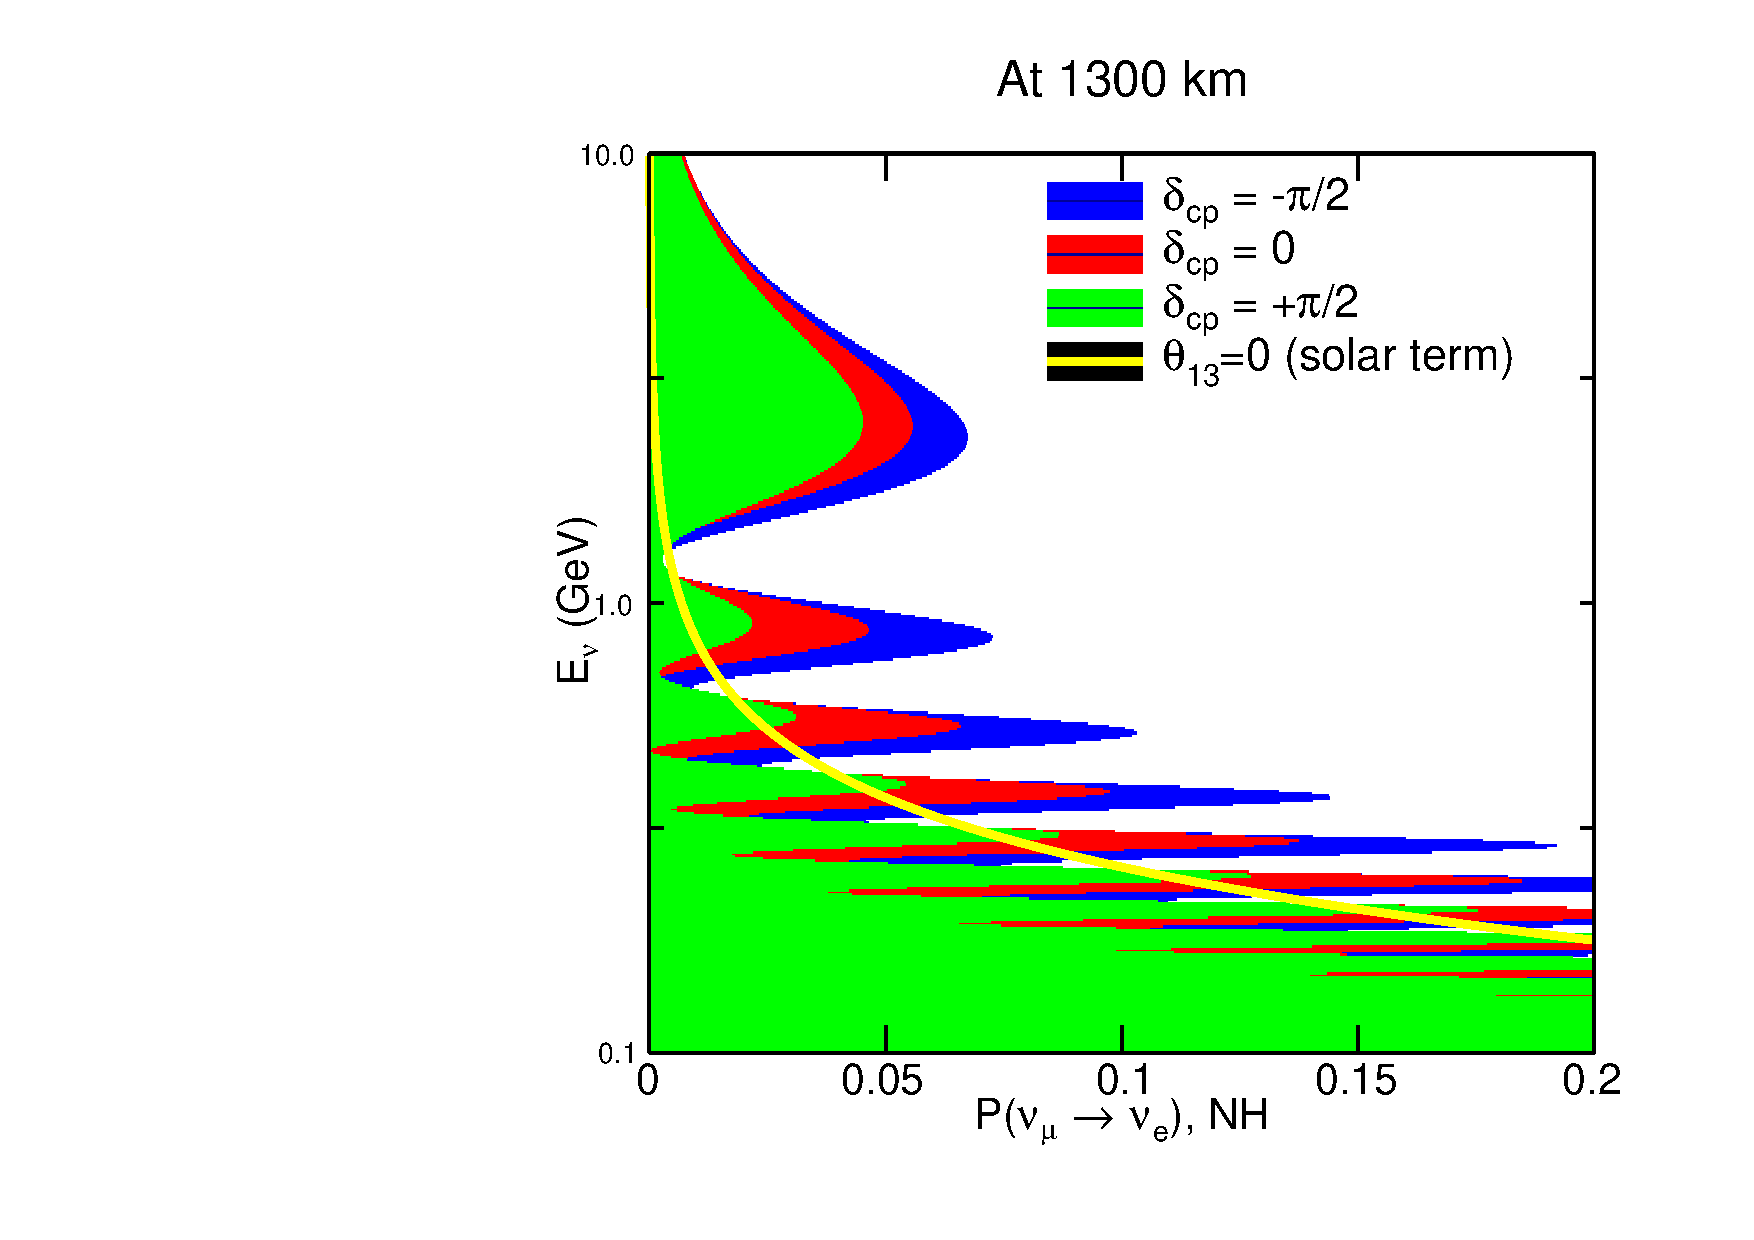
\includegraphics[width=0.45\linewidth]{energy_nu_no.pdf}
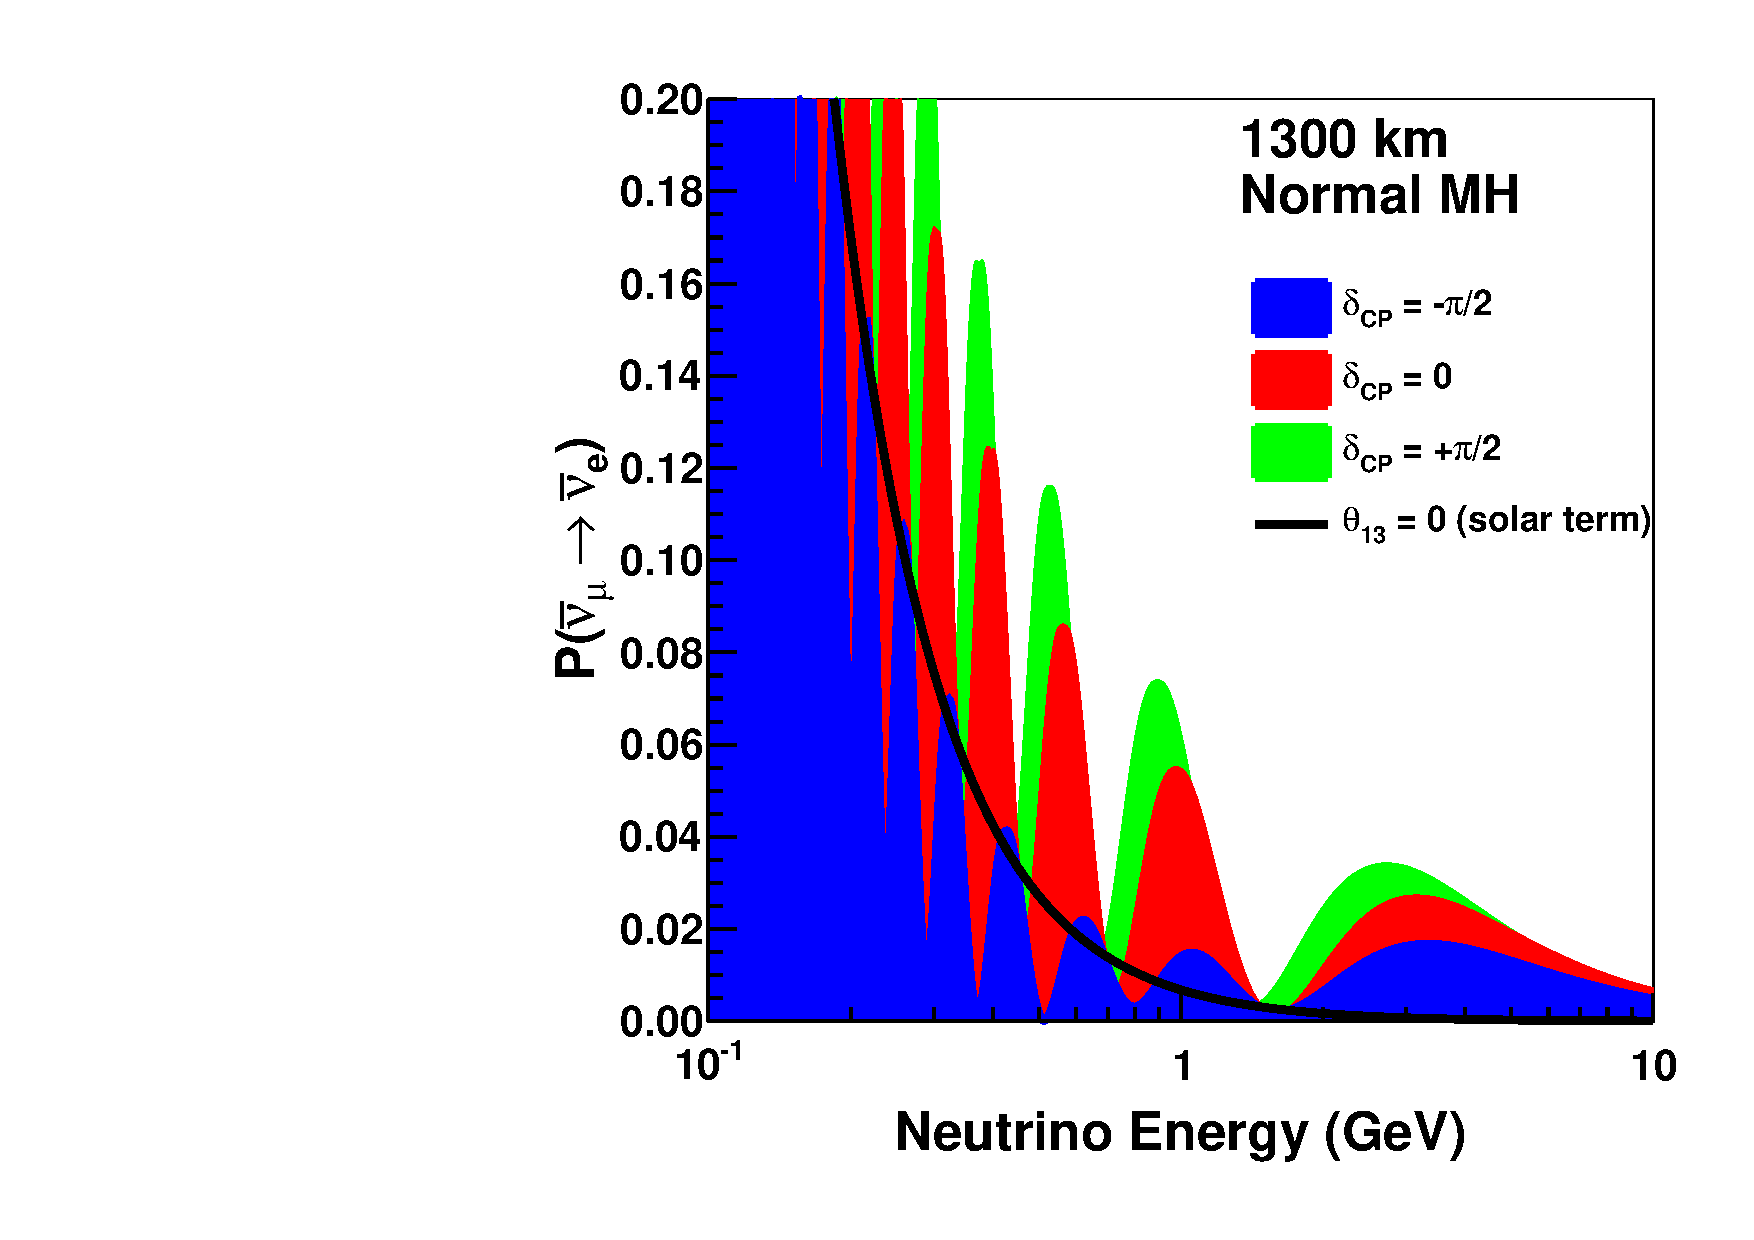
\includegraphics[width=0.45\linewidth]{energy_anu_no.pdf}
\end{cdrfigure}

The experimental sensitivities presented here are estimated using 
GLoBES\cite{Huber:2004ka,Huber:2007ji}. GLoBES takes flux simulations, cross-sections,
and detector-response parameterization as inputs. In this document we present
a range of possible physics sensitivity that depends on the design of the neutrino beam.
A conservative estimate of sensitivity is calculated using a flux simulation that is based on the reference design of the beam line as presented in \vollbnf.  A flux simulation based on an optimized beam design is used to show the goal sensitivity.  There are a range of design options that produce sensitivities in between the sensitivity of the reference beam design and optimized beam design, and further optimization is possible. The actual flux will depend upon details of the hadron production and focusing design; optimization of the beam design to maximize experimental sensitivity is a critical aspect of the experiment
design.  Table~\ref{tab:beamparam} summarizes some of the properties of the flux simulations used in the sensitivity studies.  The main differences between the two beam designs are the horn current, horn design, and decay pipe length; the choice of horn design has the biggest effect on the sensitivity. Section~\ref{sec:physics-lbnosc-beam-req} describes the flux simulations in more detail and explores the potential improvements that could be achieved by variations in the reference beam design.

\begin{cdrtable}[Beam line parameters for CDR reference and optimized designs]{lcc}{beamparam}{A comparison of the beam line parameters assumed for the CDR Reference Design flux and the Optimized Design flux used in the sensitivity calculations presented in this chapter.  Please see Section~\ref{sec:physics-lbnosc-beam-req} for the details.}
Parameter & CDR Reference Design & Optimized Design\\
\toprowrule 
 Proton Beam Energy & 80~GeV & 80~GeV \\ 
 Proton Beam Power & 1.07 MW & 1.07 MW\\
 Target & Graphite & Graphite \\
 Horn Current & 230~kA & 297~kA \\
 Horn Design & NuMI-style & Genetic Optimization \\ 
 Decay Pipe Length & 204~m & 250~m \\
 Decay Pipe Diameter & 4~m & 4~m\\
\end{cdrtable}


The signal for \nue appearance is an excess of charged-current (CC) \nue and \anue interactions over the expected background in the far detector.  The background to \nue appearance is composed of: i) CC interactions of \nue and \anue intrinsic
to the beam; ii) mis-identified \numu and \anumu CC events; 
iii) neutral current (NC) backgrounds; iv) $\nu_\tau$ and $\bar{\nu}_\tau$ CC events 
in which the $\tau$'s decay leptonically into electrons/positrons. NC and $\nu_\tau$ 
backgrounds are due to interactions of higher energy neutrinos but they contribute to 
backgrounds mainly at low energy, which is important for the sensitivity to CP violation. 

The LAr TPC performance parameters that go into the GLoBES calculation are generated using the DUNE Fast Monte Carlo (MC) simulation, which is described in detail in \cite{Adams:2013qkq}.  The Fast MC combines the simulated flux, the GENIE neutrino interaction generator~\cite{Andreopoulos:2009rq}, and a parameterized detector response that is used to simulate the reconstructed energy and momentum of each final-state particle.  The simulated energy deposition of the particles in each interaction is then used to calculate reconstructed kinematic quantities (e.~g., the neutrino energy). Event sample classifications ($\nu_e$ CC-like, $\nu_{\mu}$ CC-like, or NC-like), including mis-ID rates, are determined by the identification of lepton candidates. Lepton candidates are selected based on a variety of criteria including on particle kinematics, detector thresholds, and probabilistic estimates of particle fates. To reduce the NC and $\nu_{\tau}$ CC backgrounds in the $\nu_e$ CC-like sample, an additional discriminant is formed using reconstructed transverse momentum along with reconstructed neutrino and hadronic energy as inputs to a k-Nearest-Neighbor (kNN) machine-learning algorithm.  Figures~\ref{fig:smearing_nue}-\ref{fig:smearing_nc} show the true-to-reconstructed energy smearing matrices extracted from the Fast MC and used as inputs to GLoBES.  Figure~\ref{fig:eff} shows the analysis sample detection$\times$selection efficiencies for the various signal and background modes used by GLoBES, also extracted from the Fast MC.

\begin{cdrfigure}[\nue and\anue True-to-reconstructed energy smearing matrices]{smearing_nue}{True-to-reconstructed energy smearing matrices for CC \nue (left) and \anue (right) interactions extracted from the Fast MC and used as inputs to GLoBES.  Top: Used in the appearance sample.  Bottom: Used in the disappearance sample.}
 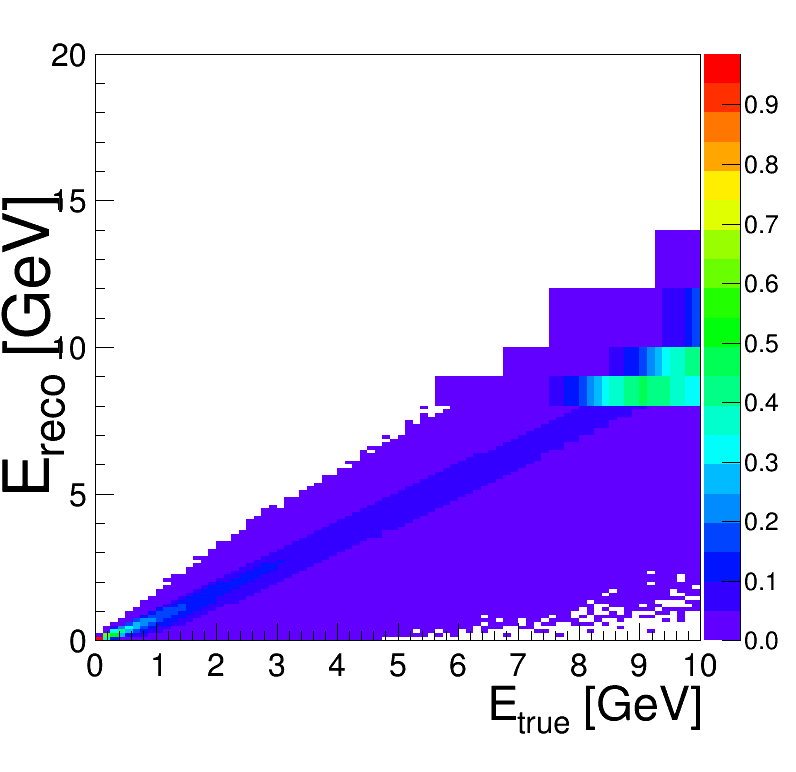
\includegraphics[width=0.49\textwidth]{LBNE_smear_plot2_nue_nominal_app.png}
 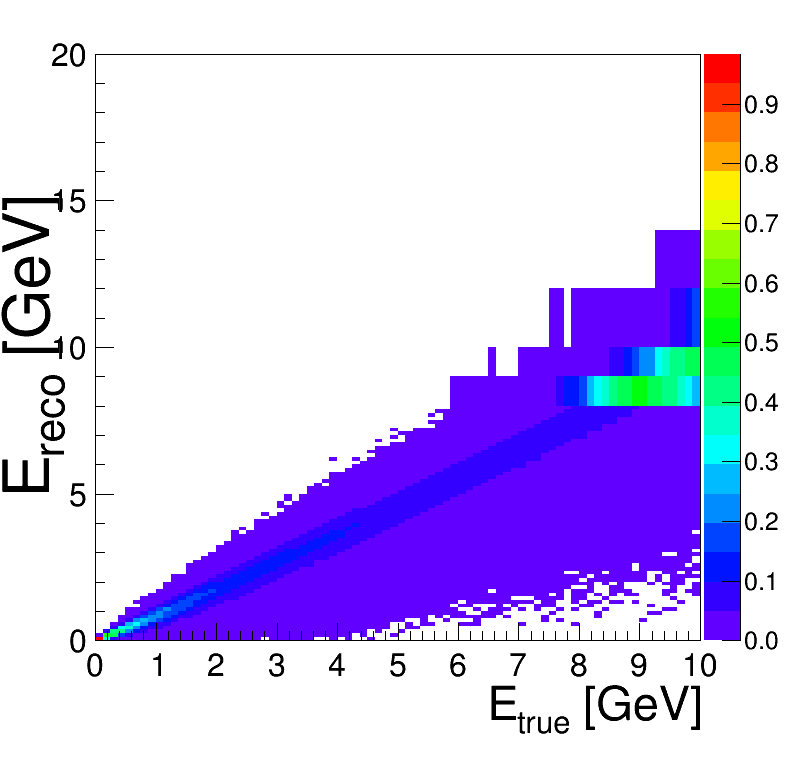
\includegraphics[width=0.49\textwidth]{LBNE_smear_plot2_anue_nominal_app.png}
 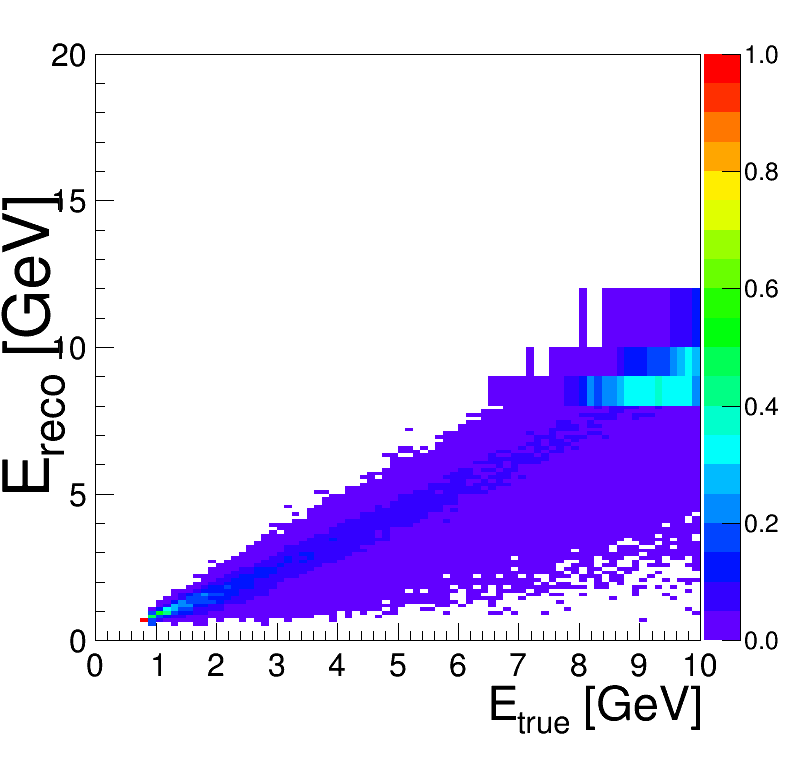
\includegraphics[width=0.49\textwidth]{LBNE_smear_plot2_nue_nominal_dis.png}
 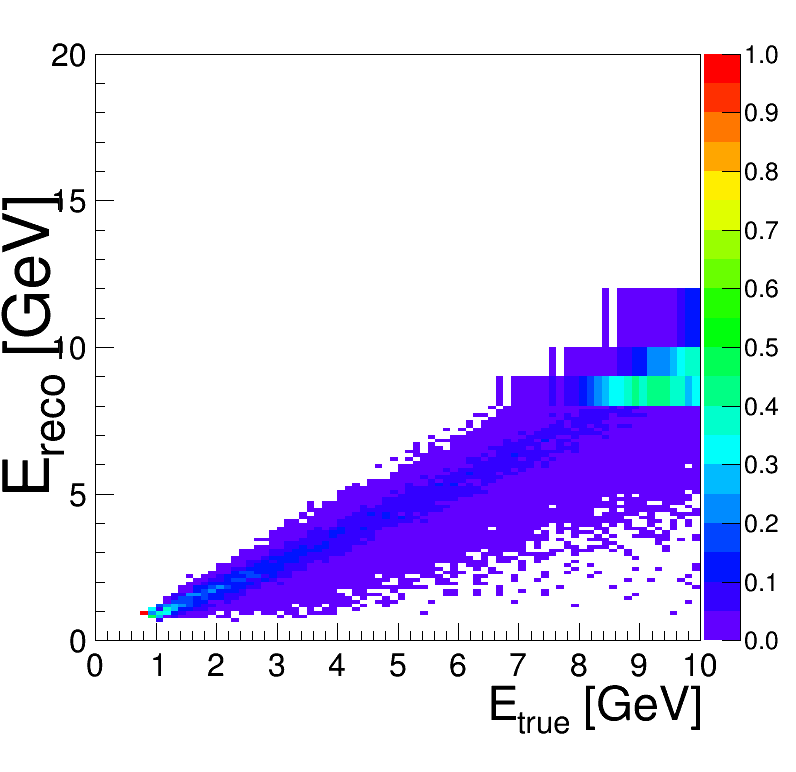
\includegraphics[width=0.49\textwidth]{LBNE_smear_plot2_anue_nominal_dis.png}
\end{cdrfigure}

\begin{cdrfigure}[\numu and\anumu True-to-reconstructed energy smearing matrices]{smearing_numu}{True-to-reconstructed energy smearing matrices for CC \numu (left) and \anumu (right) interactions extracted from the Fast MC and used as inputs to GLoBES.  Top: Used in the appearance sample.  Bottom: Used in the disappearance sample.}
 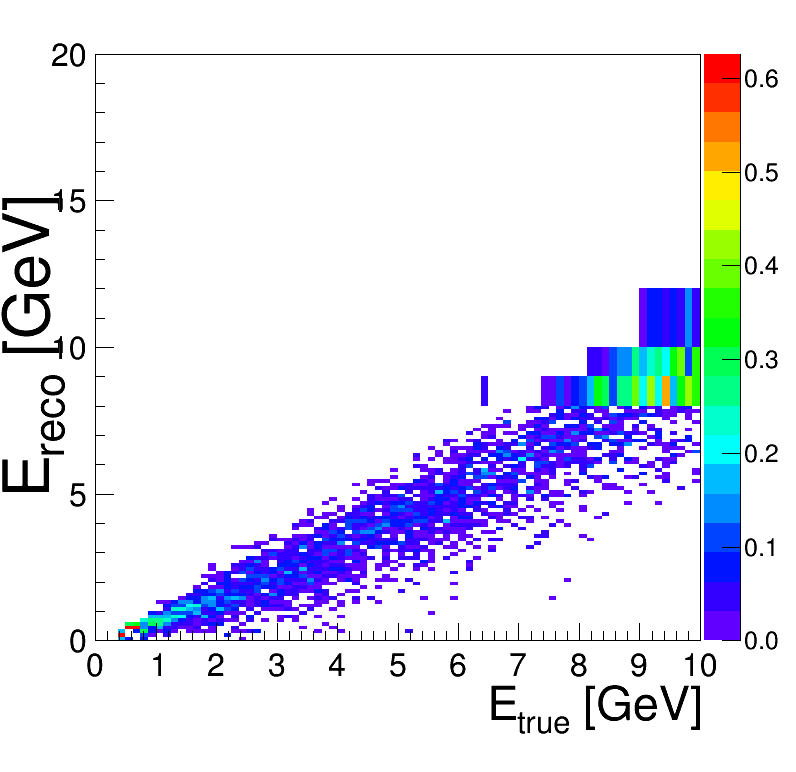
\includegraphics[width=0.49\textwidth]{LBNE_smear_plot2_numu_nominal_app.png}
 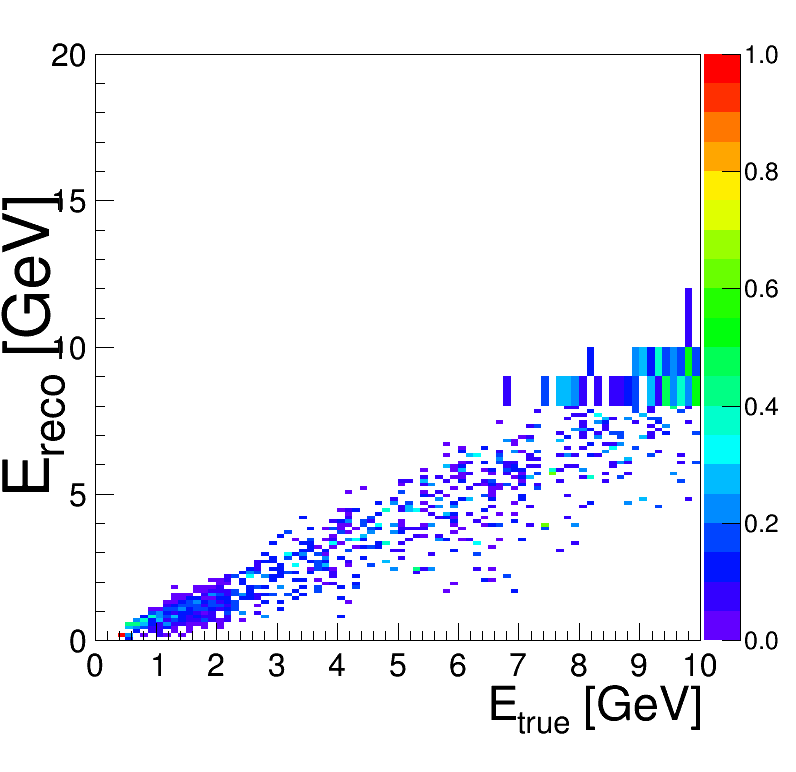
\includegraphics[width=0.49\textwidth]{LBNE_smear_plot2_anumu_nominal_app.png}
 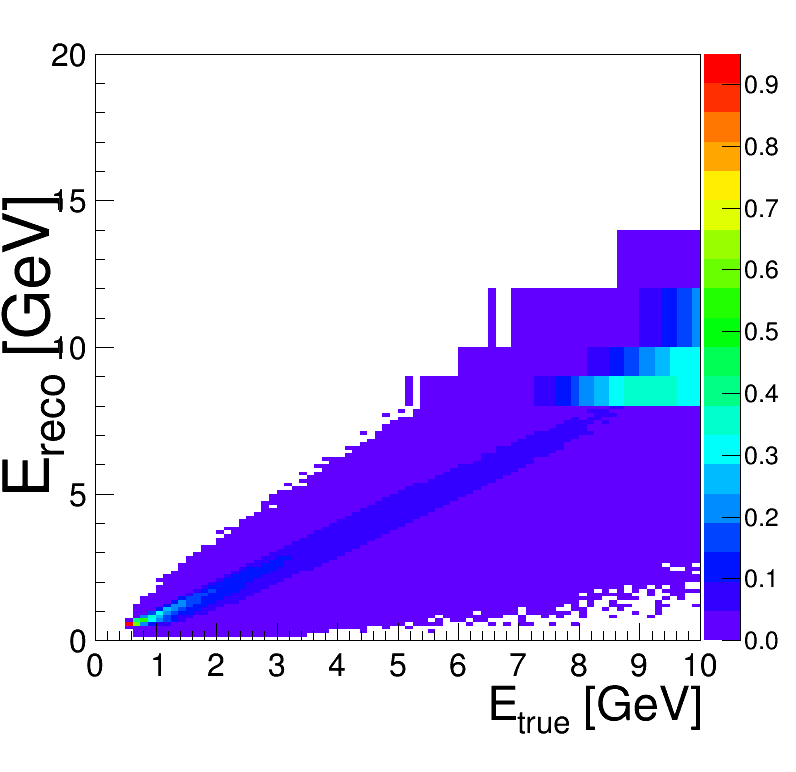
\includegraphics[width=0.49\textwidth]{LBNE_smear_plot2_numu_nominal_dis.png}
 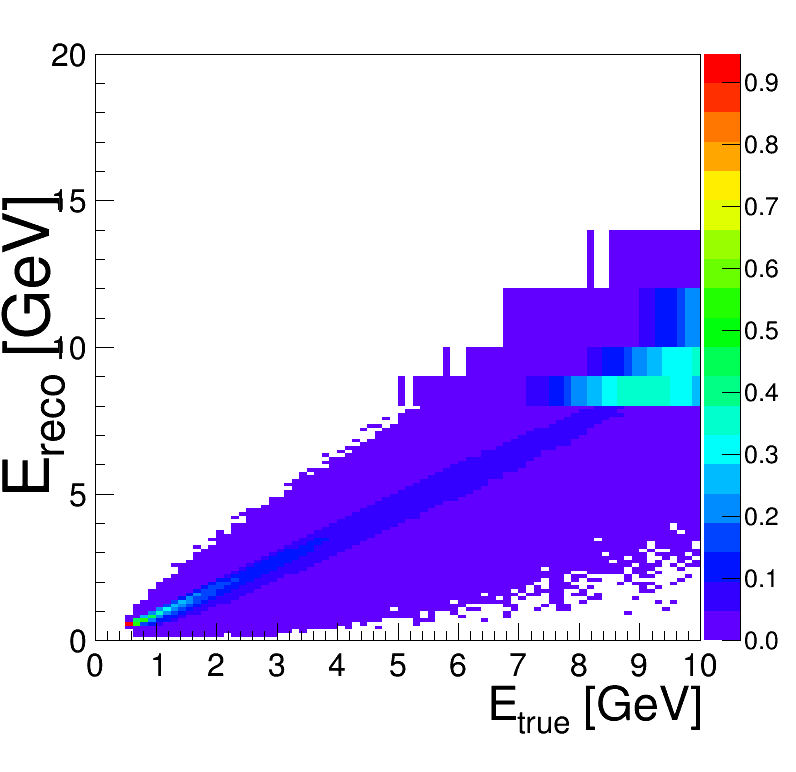
\includegraphics[width=0.49\textwidth]{LBNE_smear_plot2_anumu_nominal_dis.png}
\end{cdrfigure}

\begin{cdrfigure}[\nutau and\anutau True-to-reconstructed energy smearing matrices]{smearing_nutau}{True-to-reconstructed energy smearing matrices for CC \nutau (left) and \anutau (right) interactions extracted from the Fast MC and used as inputs to GLoBES.  Top: Used in the appearance sample.  Bottom: Used in the disappearance sample.}
 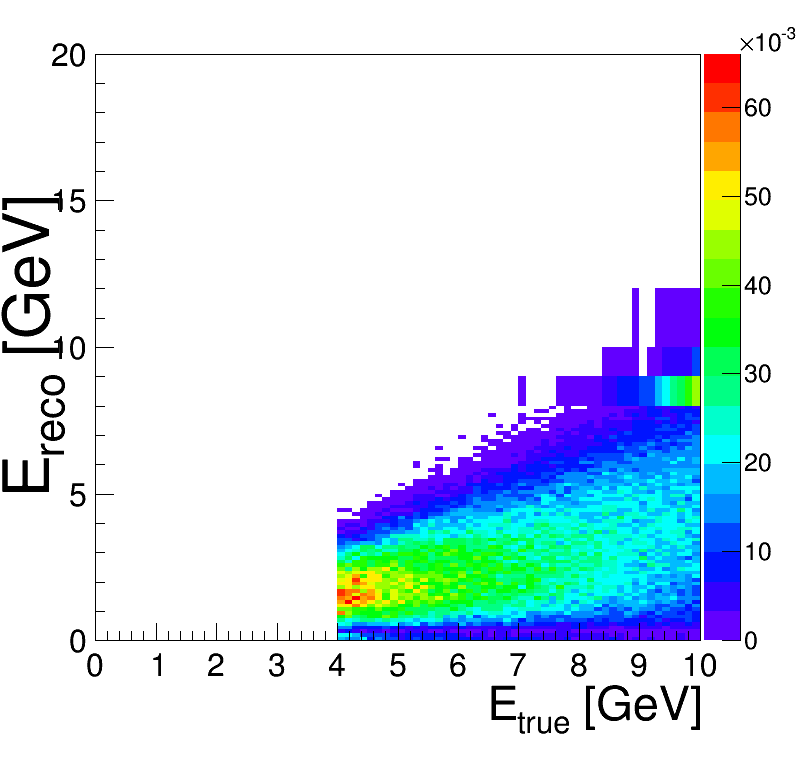
\includegraphics[width=0.49\textwidth]{LBNE_smear_plot2_nut_nominal_app.png}
 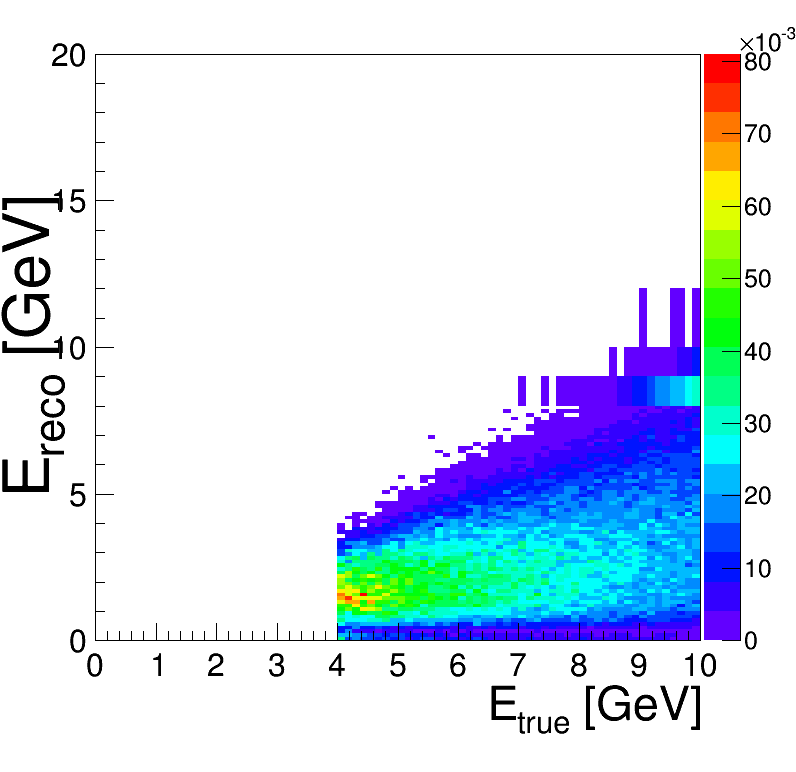
\includegraphics[width=0.49\textwidth]{LBNE_smear_plot2_anut_nominal_app.png}
 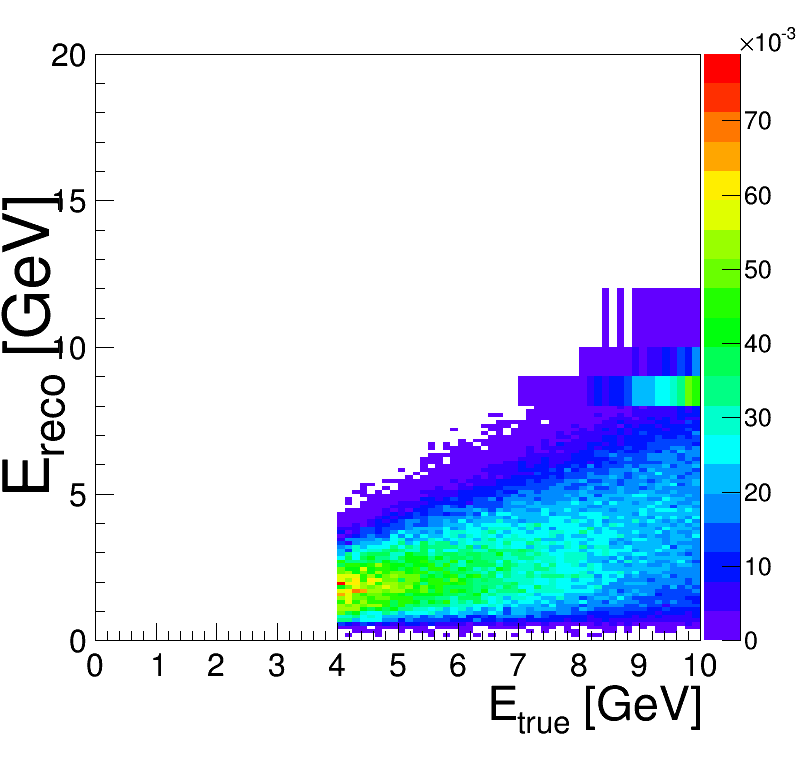
\includegraphics[width=0.49\textwidth]{LBNE_smear_plot2_nut_nominal_dis.png}
 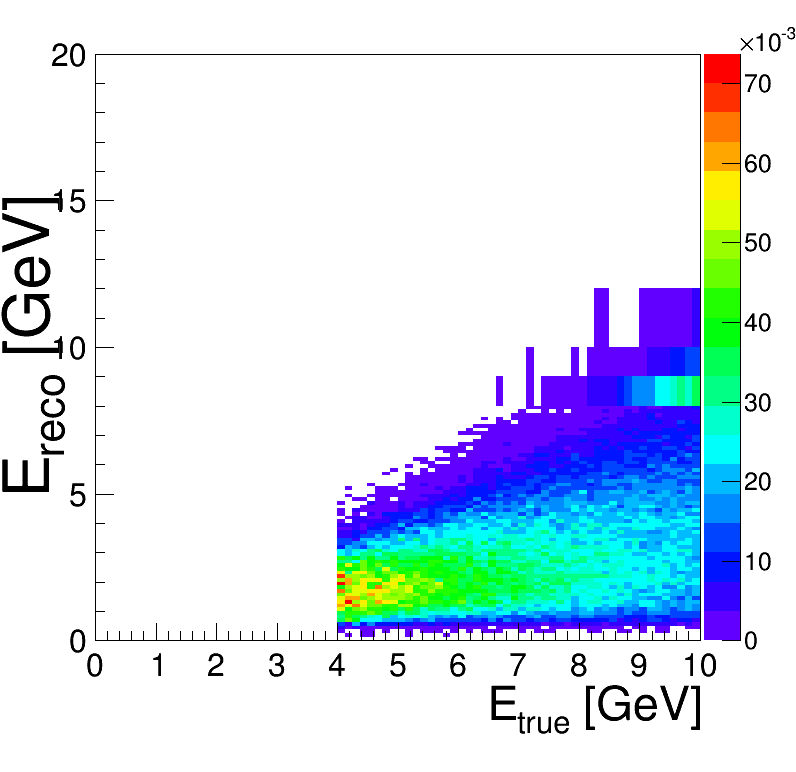
\includegraphics[width=0.49\textwidth]{LBNE_smear_plot2_anut_nominal_dis.png}
\end{cdrfigure}

\begin{cdrfigure}[NC True-to-reconstructed energy smearing matrices]{smearing_nc}{True-to-reconstructed energy smearing matrices for NC interactions extracted from the Fast MC and used as inputs to GLoBES.  Left: Used in the appearance sample.  Right: Used in the disappearance sample.}
 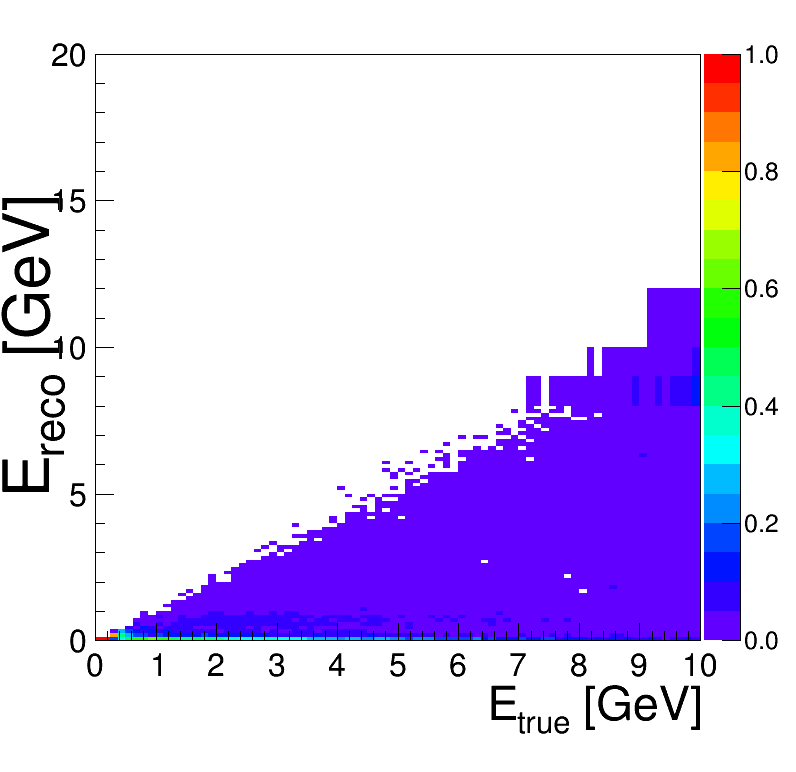
\includegraphics[width=0.49\textwidth]{LBNE_smear_plot2_NC_nominal_app.png}
 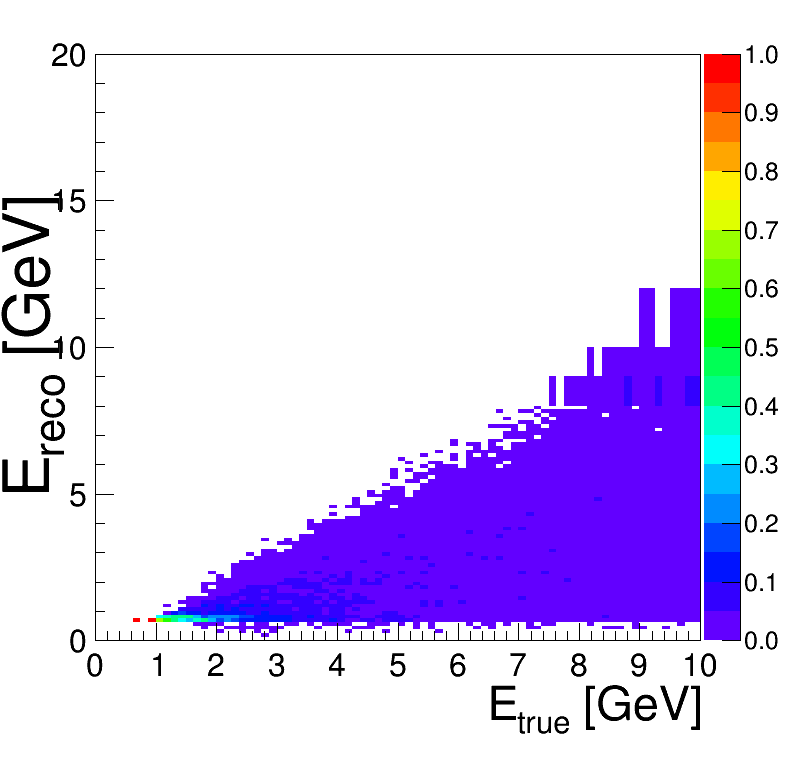
\includegraphics[width=0.49\textwidth]{LBNE_smear_plot2_NC_nominal_dis.png}
\end{cdrfigure}

\begin{cdrfigure}[Analysis sample detection $\times$ selection efficiencies]{eff}{Analysis sample detection $\times$ selection efficiencies for the various signal and background modes extracted from the Fast MC and used as inputs to GLoBES.  Top: Used in the appearance sample. Bottom: Used in the disappearance sample.  Left: Neutrino beam mode.  Right: Antineutrino beam mode. PLACEHOLDER PLOTS: WILL BE UPDATED.}
 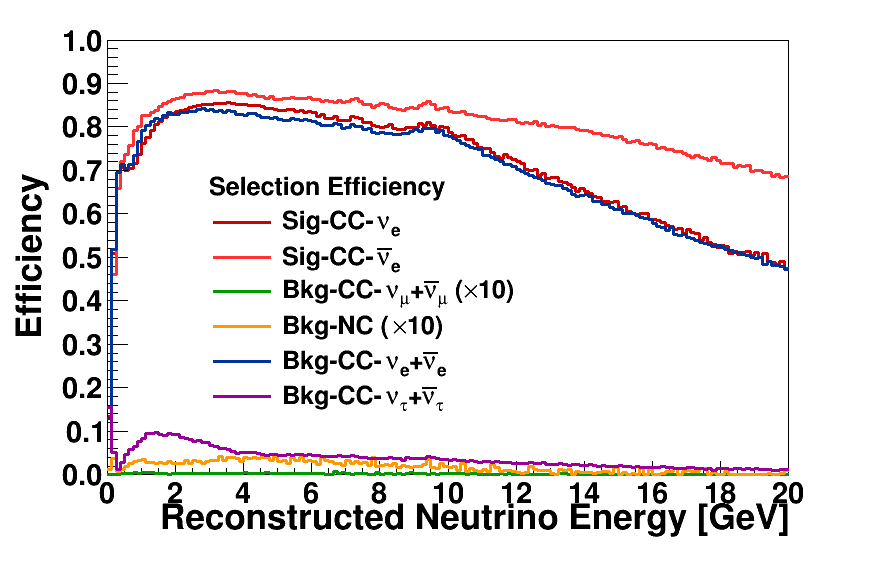
\includegraphics[width=0.49\textwidth]{LBNE_Ev_reco_app_FHC_eff.png}
 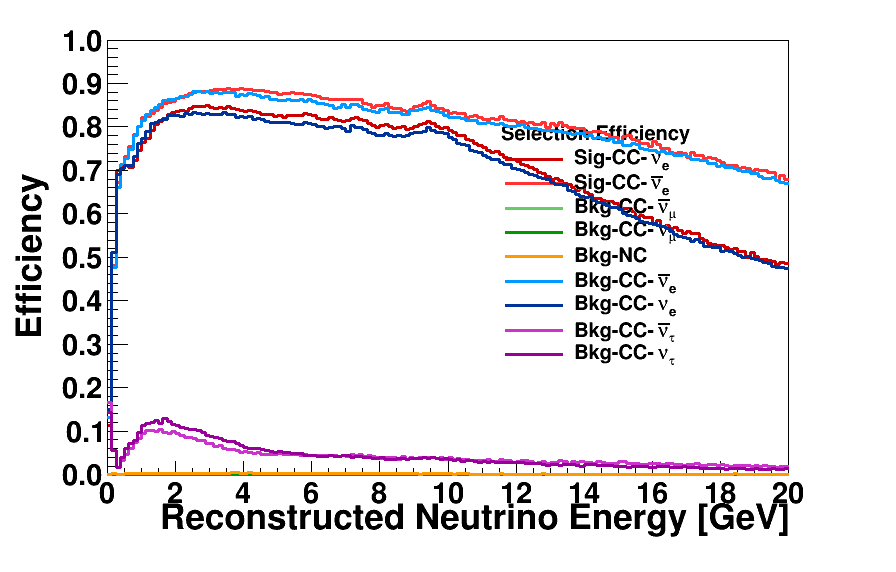
\includegraphics[width=0.49\textwidth]{LBNE_Ev_reco_app_RHC_eff.png}
 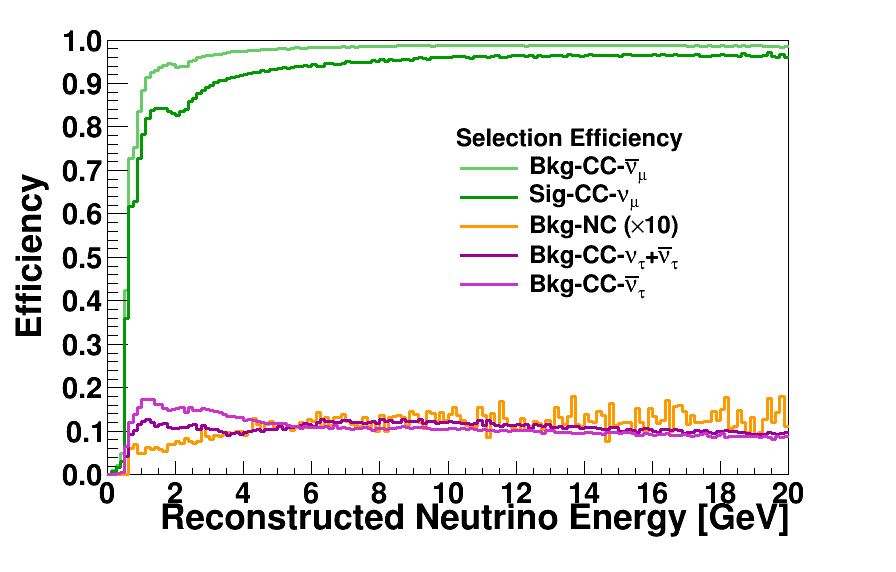
\includegraphics[width=0.49\textwidth]{LBNE_Ev_reco_dis_FHC_eff.png}
 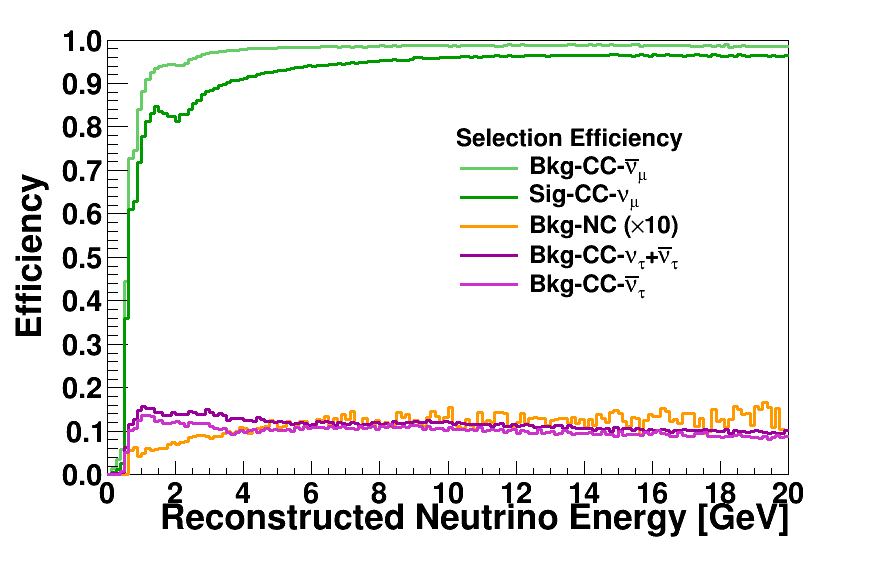
\includegraphics[width=0.49\textwidth]{LBNE_Ev_reco_dis_RHC_eff.png}
\end{cdrfigure}

 The cross-section inputs to GLoBES have been generated using GENIE 2.8.4~\cite{Andreopoulos:2009rq}.
The neutrino oscillation parameters and the uncertainty on those parameters are taken from the 
Nu-Fit~\cite{Gonzalez-Garcia:2014bfa} global fit to neutrino data; the values are given in 
Table~\ref{tab:oscpar_nufit}.  (See also \cite{Capozzi:2013csa} and \cite{Forero:2014bxa} for other recent global fits.) Most of the sensitivities 
in this chapter are shown assuming normal hierarchy; this is an arbitrary choice for simplicity of presentation.

\begin{cdrtable}[Oscillation parameter values and relative uncertainties]{lcc}{oscpar_nufit}{Central value and relative uncertainty of neutrino oscillation parameters from a global fit~\cite{Gonzalez-Garcia:2014bfa} to neutrino oscillation data. Because the probability distributions are somewhat non-Gaussian (particularly for $\theta_{23}$), the relative uncertainty is computed using 1/6 of the 3$\sigma$ allowed range from the fit, rather than the 1$\sigma$ range.   For $\theta_{23}$ and $\Delta m^2_{31}$, the best-fit values and uncertainties depend on whether normal mass hierarchy (NH) or inverted mass hierarchy (IH) is assumed.}
Parameter &    Central Value & Relative Uncertainty \\
\toprowrule
$\theta_{12}$ & 0.5843 & 2.3\% \\
$\theta_{23}$ (NH) & 0.738  & 5.9\% \\
$\theta_{23}$ (IH) & 0.864  & 4.9\% \\
$\theta_{13}$ & 0.148  & 2.5\% \\
$\Delta m^2_{21}$ & 7.5$\times10^{-5}$~eV$^2$ & 2.4\% \\
$\Delta m^2_{31}$ (NH) & 2.457$\times10^{-3}$~eV$^2$ &  2.0\% \\
$\Delta m^2_{31}$ (IH) & -2.449$\times10^{-3}$~eV$^2$ &  1.9\% \\
\end{cdrtable}

Figures~\ref{fig:appspectra} and~\ref{fig:disspectra} 
show the expected event rate for \nue appearance and \numu disappearance, respectively, including
expected flux, cross-section, and oscillation probabilities as a function 
of neutrino energy at a baseline of 1300~km. The spectra are shown for a 150~kt-MW-yr exposure in both neutrino and antineutrino mode, for a total 300~kt-MW-yr exposure.  The optimized beam design results in an increased signal rate in the lower energy region. Tables~\ref{tab:apprates} and~\ref{tab:disrates} give the integrated rate between 0.5 and 8.0~GeV for the appearance and disappearance spectra, respectively.  The spectra and rates are shown for both the reference beam design and the optimized beam design.

\begin{cdrfigure}[\nue and \anue appearance spectra]{appspectra}{\nue and \anue appearance spectra: Reconstructed energy distribution of selected $\nu_e$ CC-like events assuming a 150~kt-MW-yr exposure in the neutrino-beam mode (left) and antineutrino-beam mode (right), for a total 300~kt-MW-yr exposure.  The plots assume normal mass hierarchy and $\mdeltacp = 0$.  The spectra are shown for both the CDR reference beam design and the optimized beam design as described in Section~\ref{sec:physics-lbnosc-beam-req}.}
 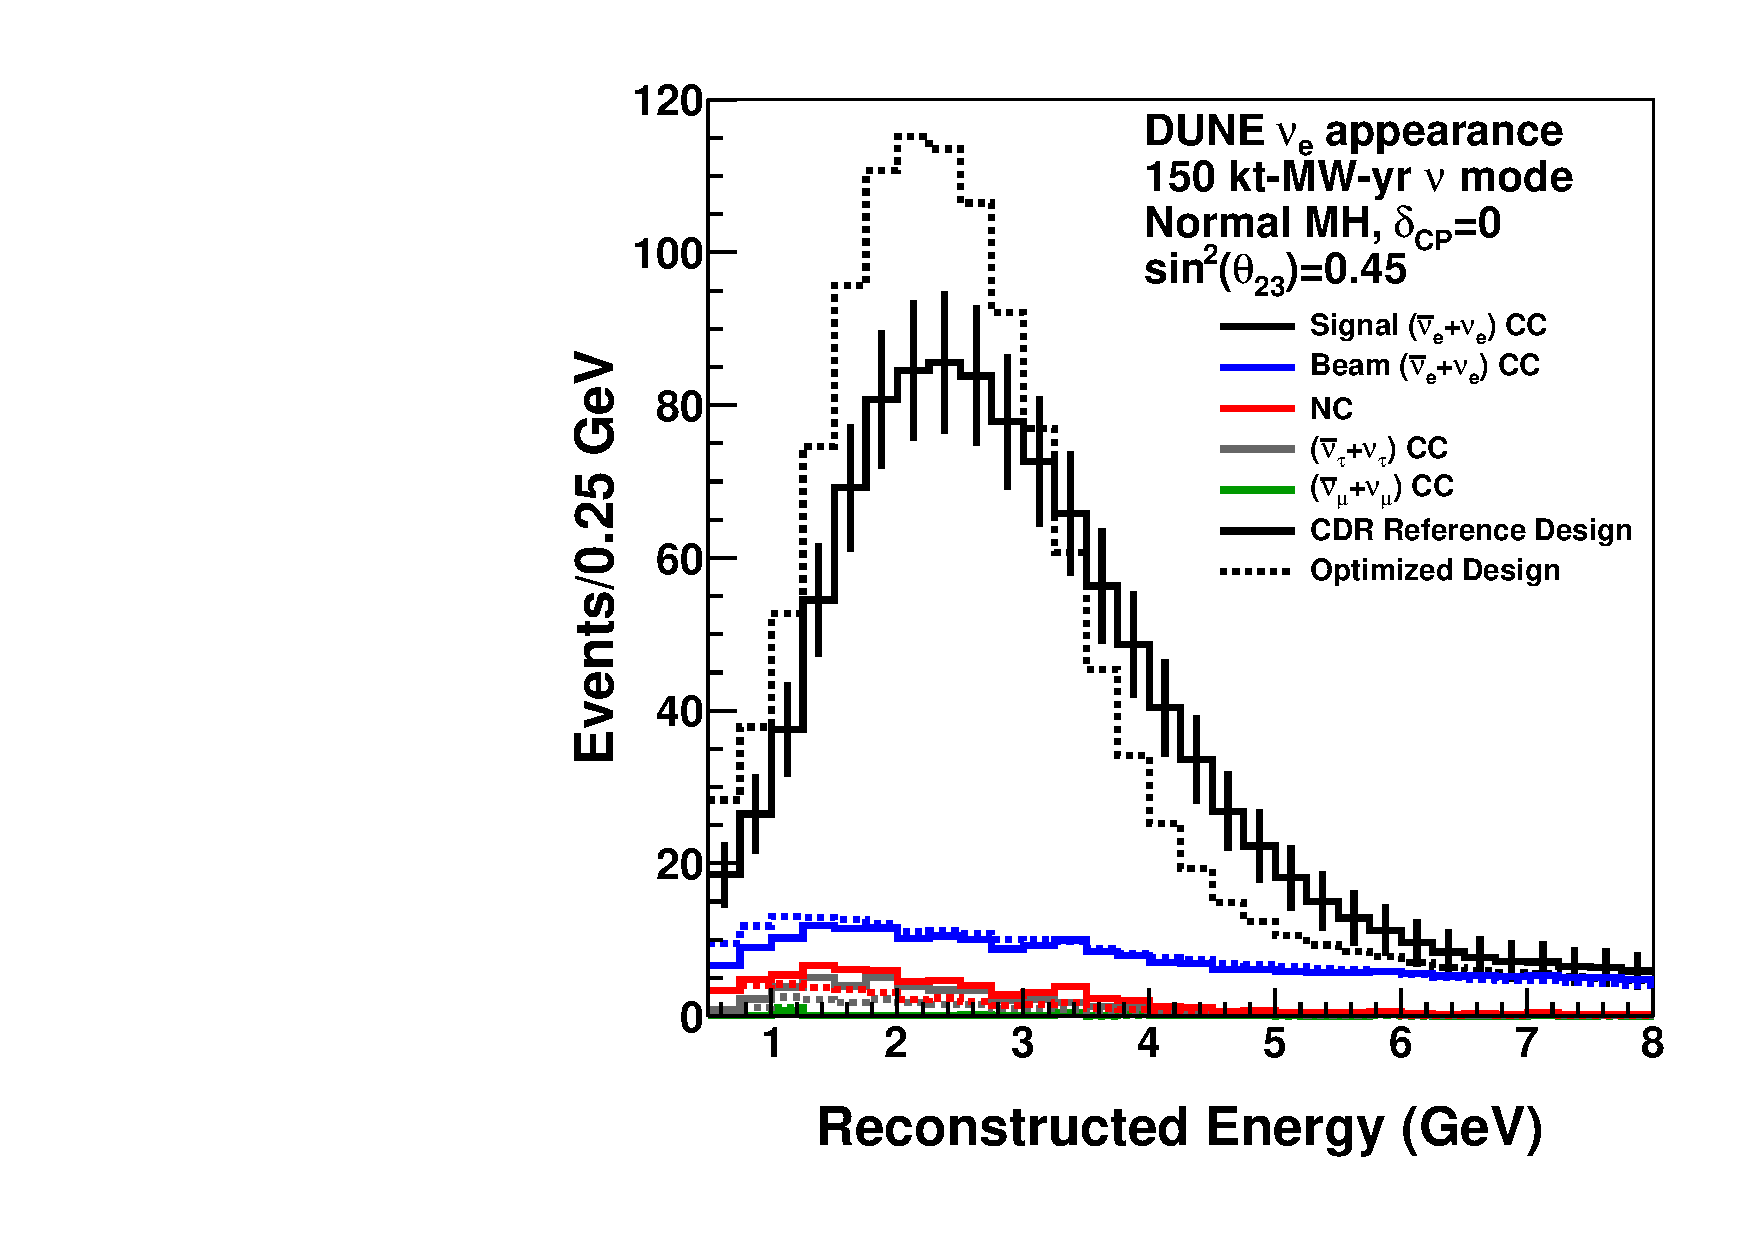
\includegraphics[width=0.49\textwidth]{NueApp_NH.pdf}
 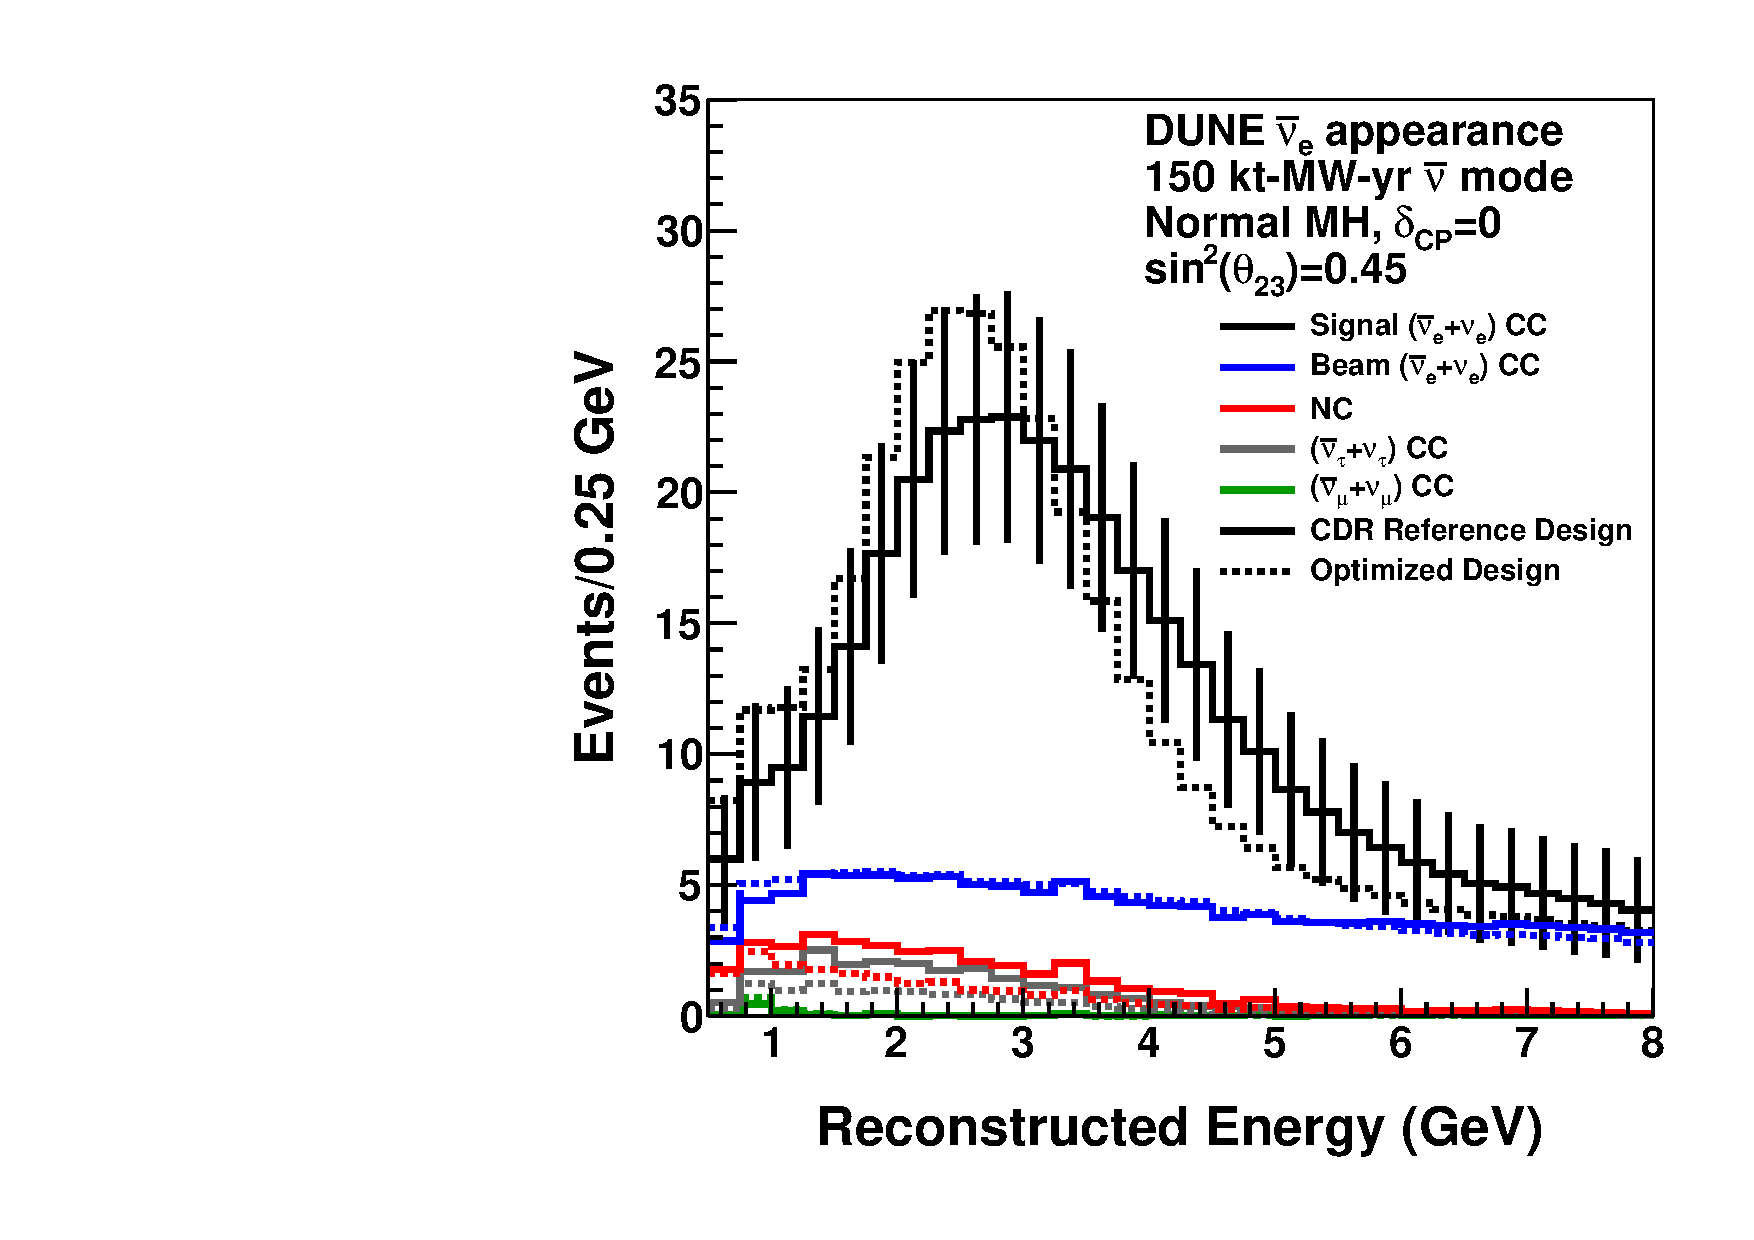
\includegraphics[width=0.49\textwidth]{NueBarApp_NH.pdf}
\end{cdrfigure}

\begin{cdrfigure}[\numu and \anumu disappearance spectra]{disspectra}{\numu and \anumu disappearance spectra: Reconstructed energy distribution of selected $\nu_{\mu}$ CC-like events assuming a 150~kt-MW-yr exposure in the neutrino-beam mode (left) and antineutrino-beam mode (right), for a total 300~kt-MW-yr exposure.  The plots assume normal mass hierarchy and $\mdeltacp = 0$.  The spectra are shown for both the CDR reference beam design and the optimized beam design as described in Section~\ref{sec:physics-lbnosc-beam-req}.}
 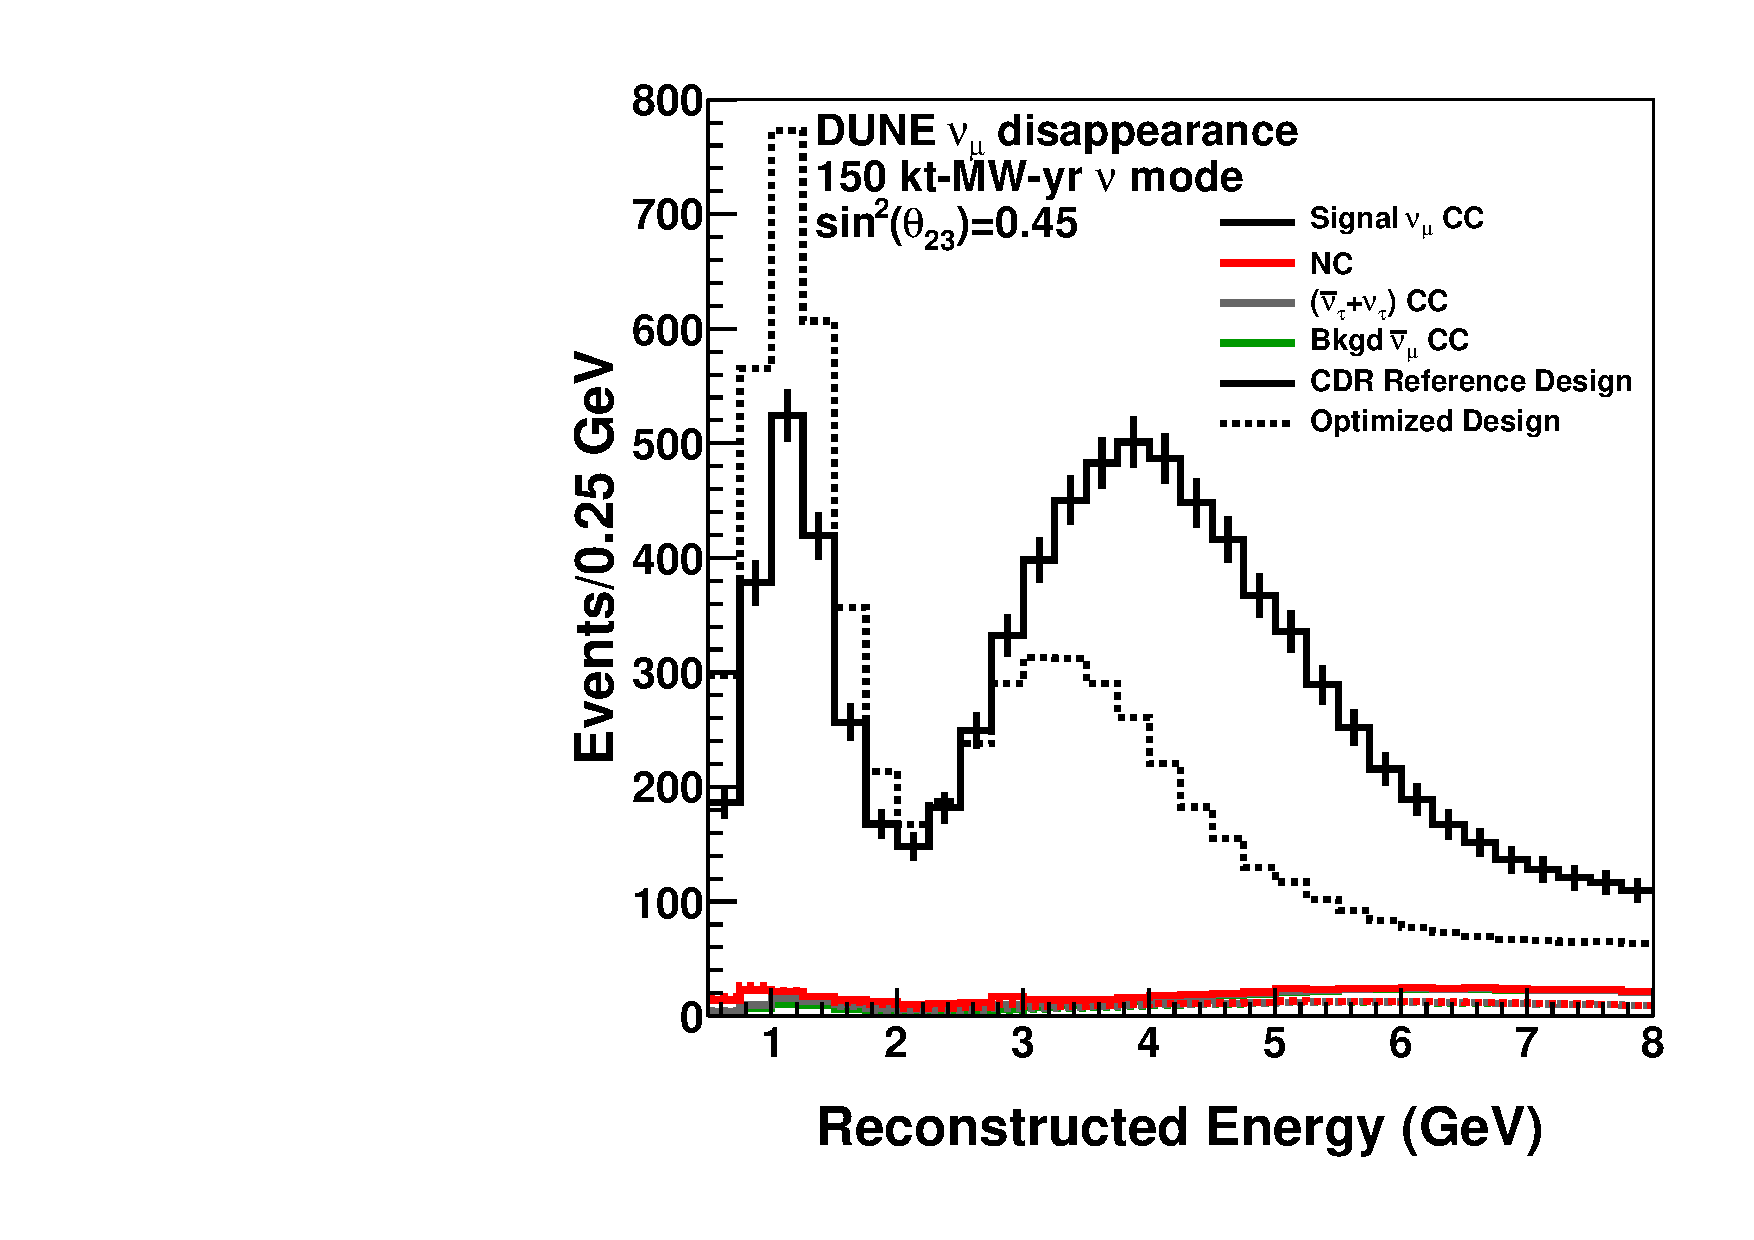
\includegraphics[width=0.49\textwidth]{NumuDis.pdf}
 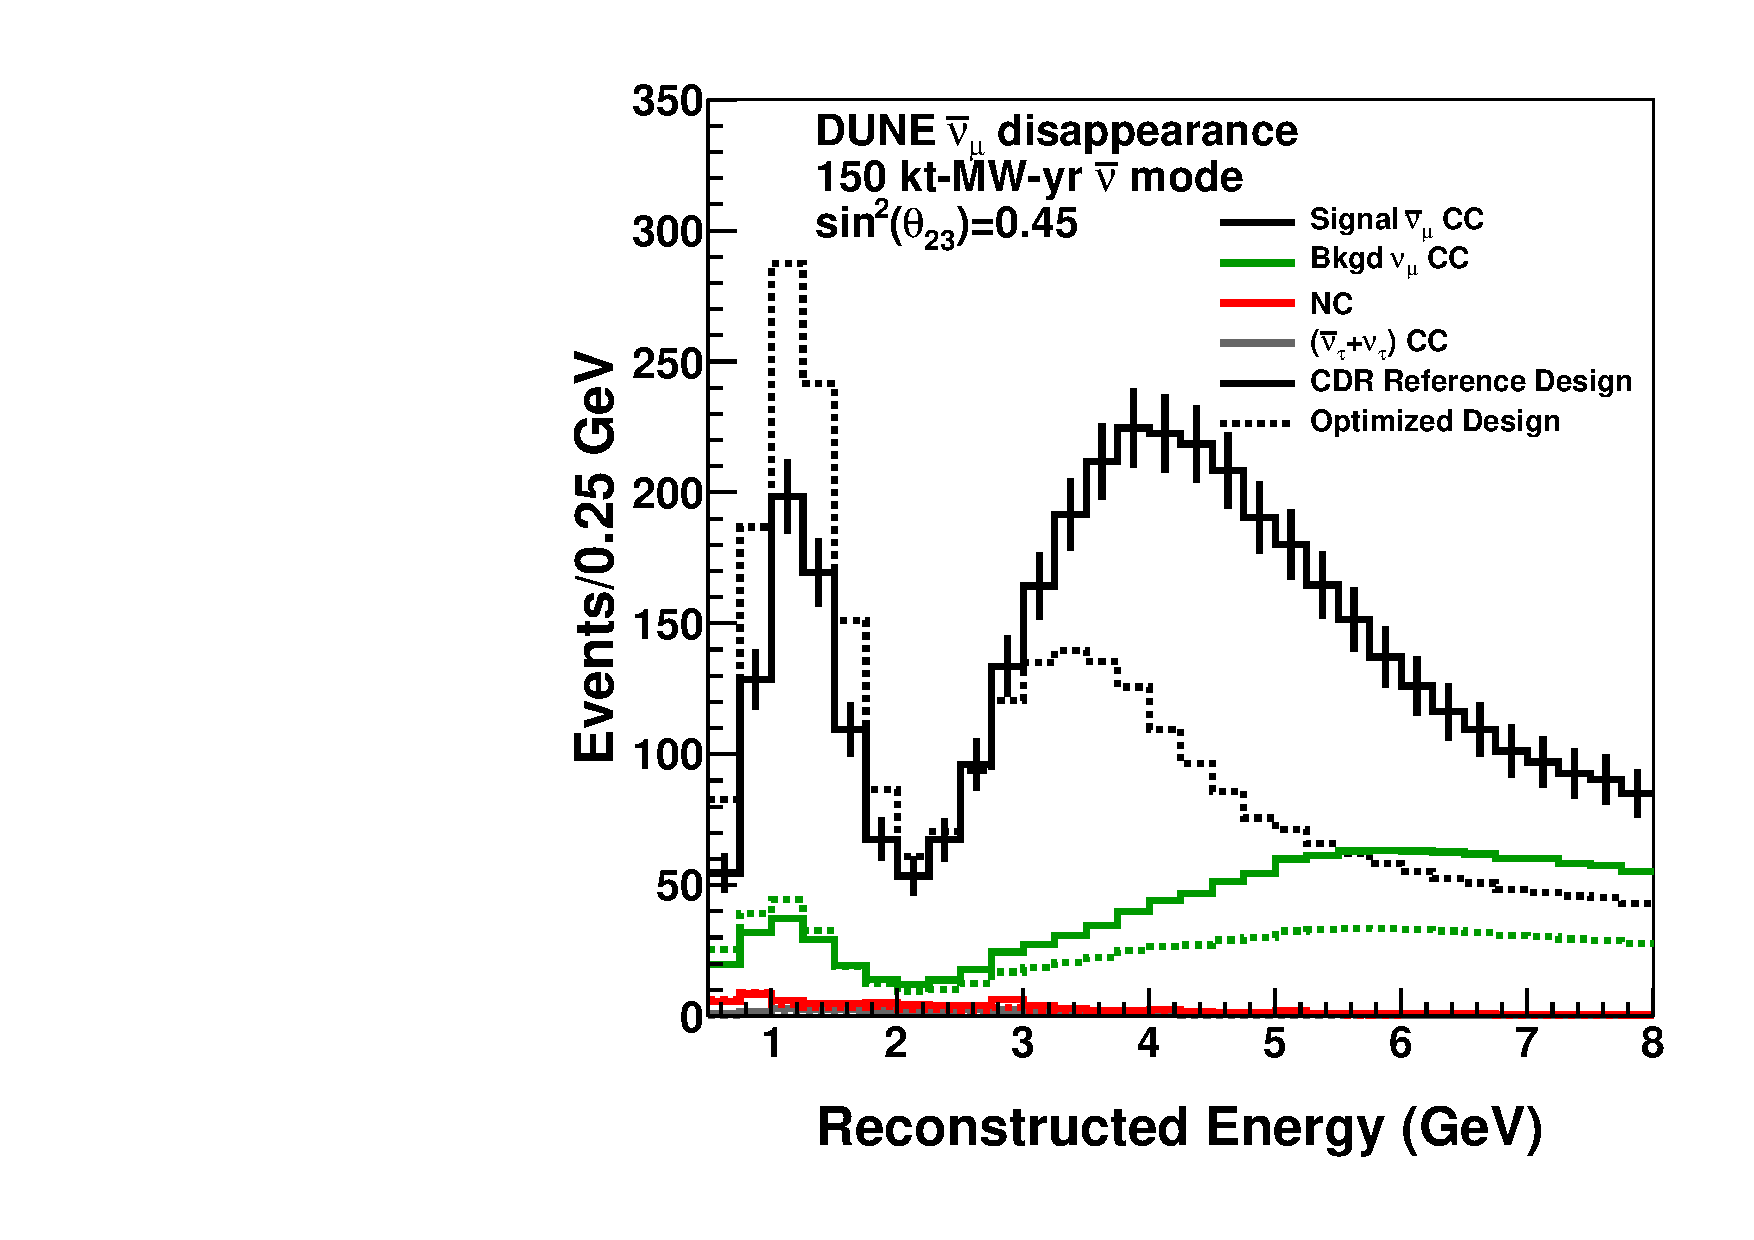
\includegraphics[width=0.49\textwidth]{NumuBarDis.pdf}
\end{cdrfigure}

\begin{cdrtable}[\nue and \anue appearance rates]{lcc}{apprates}{\nue and \anue appearance rates: Integrated rate of selected $\nu_e$ CC-like events between 0.5 and 8.0~GeV assuming a 150~kt-MW-yr exposure in the neutrino-beam mode and antineutrino-beam mode.  The signal rates are shown for both normal mass hierarchy (NH) and inverted mass hierarchy (IH), and all the background rates assume normal mass hierarchy.  All the rates assume $\mdeltacp = 0$, and the rates are shown for both the CDR reference beam design and the optimized beam as described in Section~\ref{sec:physics-lbnosc-beam-req}.}
  & CDR Reference Design & Optimized Design\\
  \toprowrule
  \toprowrule
 $\nu$ mode (150~kt-MW-yr) & & \\
 \toprowrule
 \nue Signal NH (IH) & 881 (510) & 968 (538)\\
 \anue Signal NH (IH) & 17 (29) & 11 (23)\\
 \toprowrule
 Total Signal NH (IH) & 898 (539) & 979 (561) \\
 \toprowrule
 Beam $\nu_{e}+\bar{\nu}_{e}$ CC Bkgd & 284 & 293 \\
 NC Bkgd & 30 & 26 \\
 $\nu_{\tau}+\bar{\nu}_{\tau}$ CC Bkgd & 43 & 20 \\
 $\nu_{\mu}+\bar{\nu}_{\mu}$ CC Bkgd & 3 & 3 \\
 \toprowrule
 Total Bkgd & 360 & 342 \\
 \toprowrule
 \toprowrule
 $\bar{\nu}$ mode (150~kt-MW-yr) & & \\
 \toprowrule
 \nue Signal NH (IH) & 68 (43) & 52 (31)\\
 \anue Signal NH (IH) & 172 (383) & 173 (441)\\
 \toprowrule
 Total Signal NH (IH) & 240 (426) & 225 (472) \\
 \toprowrule
 Beam $\nu_{e}+\bar{\nu}_{e}$ CC Bkgd & 177 & 173 \\
 NC Bkgd & 16 & 13 \\
 $\nu_{\tau}+\bar{\nu}_{\tau}$ CC Bkgd & 24 & 11 \\
 $\nu_{\mu}+\bar{\nu}_{\mu}$ CC Bkgd & 2 & 2 \\
 \toprowrule
 Total Bkgd & 219 & 199 \\
\end{cdrtable}

\begin{cdrtable}[\numu and \anumu disappearance rates]{lcc}{disrates}{\numu and \anumu disappearance rates: Integrated rate of selected $\nu_{\mu}$ CC-like events between 0.5 and 8.0~GeV assuming a 150~kt-MW-yr exposure in the neutrino-beam mode and antineutrino-beam mode.  The rates are shown for normal mass hierarchy and $\mdeltacp = 0$, and the rates are shown for both the CDR reference beam design and the optimized beam as described in Section~\ref{sec:physics-lbnosc-beam-req}.}
  & CDR Reference Design & Optimized Design\\
  \toprowrule
  \toprowrule
 $\nu$ mode (150~kt-MW-yr) & & \\
 \toprowrule
 \numu Signal & 10842 & 7929 \\
 \toprowrule
  \anumu CC Bkgd & 958 & 511 \\
 NC Bkgd & 88 & 76 \\
 $\nu_{\tau}+\bar{\nu}_{\tau}$ CC Bkgd & 63 & 29 \\
%  \toprowrule
%  Total Bkgd & 1109 & 616 \\
 \toprowrule
 \toprowrule
 $\bar{\nu}$ mode (150~kt-MW-yr) & & \\
 \toprowrule
 \anumu Signal & 3754 & 2639 \\
 \toprowrule
  \numu CC Bkgd & 2598 & 1525 \\
 NC Bkgd & 50 & 41 \\
 $\nu_{\tau}+\bar{\nu}_{\tau}$ CC Bkgd & 39 & 18 \\
%  \toprowrule
%  Total Bkgd & 2687 & 1584 \\
\end{cdrtable}

Sensitivity to determination of the neutrino mass hierarchy and discovery
of CP violation are obtained by
simultaneously fitting the $\nu_\mu \rightarrow \nu_\mu$,
$\overline{\nu}_\mu \rightarrow \overline{\nu}_\mu$, $\nu_\mu \rightarrow \nu_e$, 
and  $\overline{\nu}_\mu \rightarrow \overline{\nu}_e$ oscillated spectra.  We assume 50\% of the total exposure comes in neutrino beam mode and 50\% in antineutrino beam mode.  A 50\%/50\% ratio of neutrino to antineutrino data has been shown to produce a nearly optimal sensitivity, and small deviations from this (e.g., 40\%/60\%, 60\%/40\%) produce negligible changes in the sensitivity.

The neutrino oscillation parameters are all
allowed to vary, constrained by a Gaussian prior with 1$\sigma$ width given
by the relative uncertainties shown in Table~\ref{tab:oscpar_nufit}.
The effect of systematic uncertainty
is approximated using signal and background normalization uncertainties, which
are treated as 100\% uncorrelated among the four samples.
The baseline systematic uncertainty estimates and the effect
of considering larger signal and background normalization uncertainties are
discussed in Section~\ref{sec:physics-lbnosc-beamnd-req}. 

In these fits, experimental sensitivity is
quantified using a test statistic, $\Delta\chi^2$, which is calculated
by comparing the predicted spectra for alternate hypotheses.
These quantities are defined, differently for neutrino mass hierarchy
and CP violation sensitivity, to be:
\begin{eqnarray}
\Delta\chi^2_{MH} & = & \chi^2_{IH} - \chi^2_{NH}\textrm{ (true normal hierarchy),}\label{eq:dx2_MH}\\ 
\Delta\chi^2_{MH} & = & \chi^2_{NH} - \chi^2_{IH}\textrm{ (true inverted hierarchy),}\\
\Delta\chi^2_{CPV} & = & Min[\Delta\chi^2_{CP}(\mdeltacp^{test}=0),\Delta\chi^2_{CP}(\mdeltacp^{test}=\pi)]\textrm{, where} \\
\Delta\chi^2_{CP} & = & \chi^2_{\mdeltacp^{test}} - \chi^2_{\mdeltacp^{true}}.\label{eq:dx2_CP} \\ \nonumber
\end{eqnarray}
Since the true value of $\mdeltacp$ is unknown, a scan is  performed over
all possible values of $\mdeltacp^{true}$. 
We define a ``typical experiment'' as one with the most probable data given a set of input parameters, 
i.e. in which no statistical fluctuations have been applied.
In this case, the predicted spectra and the true spectra are identical;
for the example of CP violation, $\chi^2_{\mdeltacp^{true}}$ 
is identically zero and the $\Delta\chi^2_{CP}$ value for a typical experiment is given by 
$\chi^2_{\mdeltacp^{test}}$.
%Add octant chi2, calculation of resolutions?

\section{Mass Hierarchy}
\label{sec:physics-lbnosc-mh}

The 1300~km baseline establishes one of DUNE's key strengths: sensitivity to the matter
effect. This effect leads to a large asymmetry in the
$\nu_\mu\to \nu_e$ versus $\overline{\nu}_\mu \to \overline{\nu}_e$
oscillation probabilities, the sign of which depends on the mass
hierarchy (MH).  At 1300~km this asymmetry is approximately
$\pm 40\%$ in the region of the peak flux; this is larger than the
maximal possible CP-violating asymmetry associated with \deltacp,
meaning that both the MH and \deltacp can be
determined unambiguously with high confidence within the same
experiment using the beam neutrinos.  DUNE's goal is to determine the MH with a significance of at least $\sqrt{\overline{\Delta\chi^{2}}} = 5$ for all \deltacp values using beam neutrinos.  Concurrent analysis of the corresponding atmospheric-neutrino samples will improve the precision with which the
MH is resolved. 

Figure~\ref{fig:mh_nominal} shows the significance with which the MH can be determined as a function of the value of \deltacp, for an exposure of 300~kt-MW-yr, which corresponds to seven years of data (3.5 years in neutrino mode plus 3.5 years in antineutrino mode) with a 40-kt detector and a 1.07-MW beam.  For this exposure, the MH is determined with a minimum significance of $\sqrt{\overline{\Delta\chi^{2}}} = 5$ for 100\% of the \deltacp values for the optimized beam design and nearly 100\% of \deltacp values for the CDR reference beam design.  Figure~\ref{fig:mh_exposure} shows the significance with which the MH can be determined for 100\% of \deltacp values as a function of exposure.  Minimum exposures of approximately 400~kt-MW-yr and 250~kt-MW-yr are required to determine the MH with a significance of $\sqrt{\overline{\Delta\chi^2}} = 5$ for 100\% of \deltacp values for the CDR reference beam design and the optimized beam design, respectively.

\begin{cdrfigure}[Mass hierarchy sensitivity for a 300~kt-MW-yr exposure]{mh_nominal}{The significance with which the mass hierarchy can be determined as a function of the value of \deltacp for an exposure of 300~kt-MW-yr assuming normal MH (left) or inverted MH (right).  The shaded region represents the range in sensitivity due to potential variations in the beam design.}
 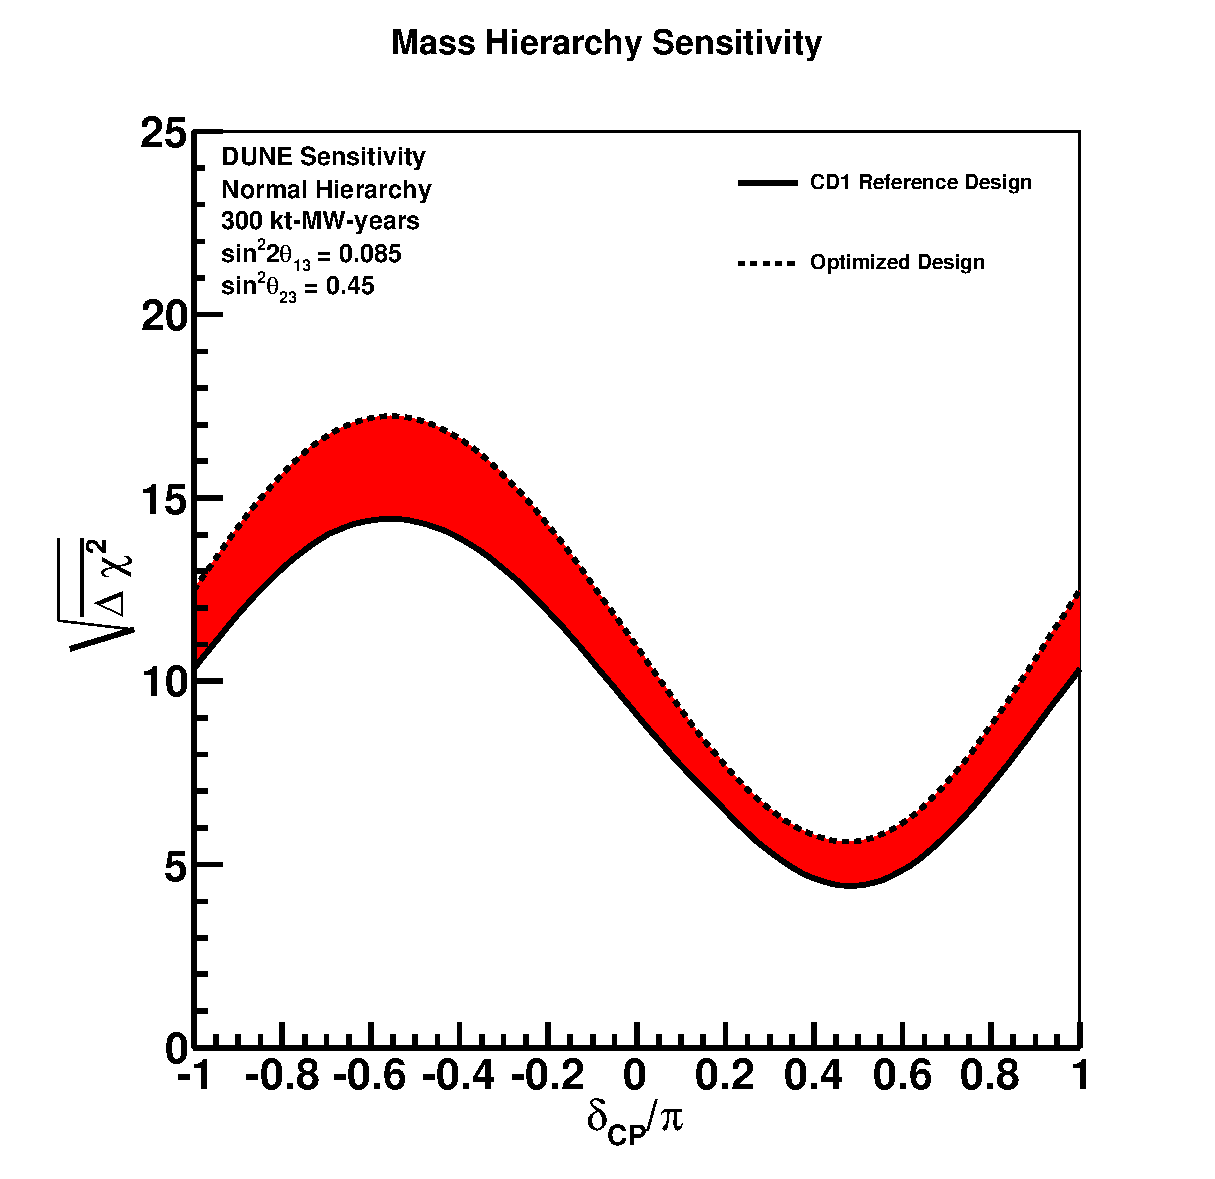
\includegraphics[width=0.49\textwidth]{mh_300ktmwyear}
 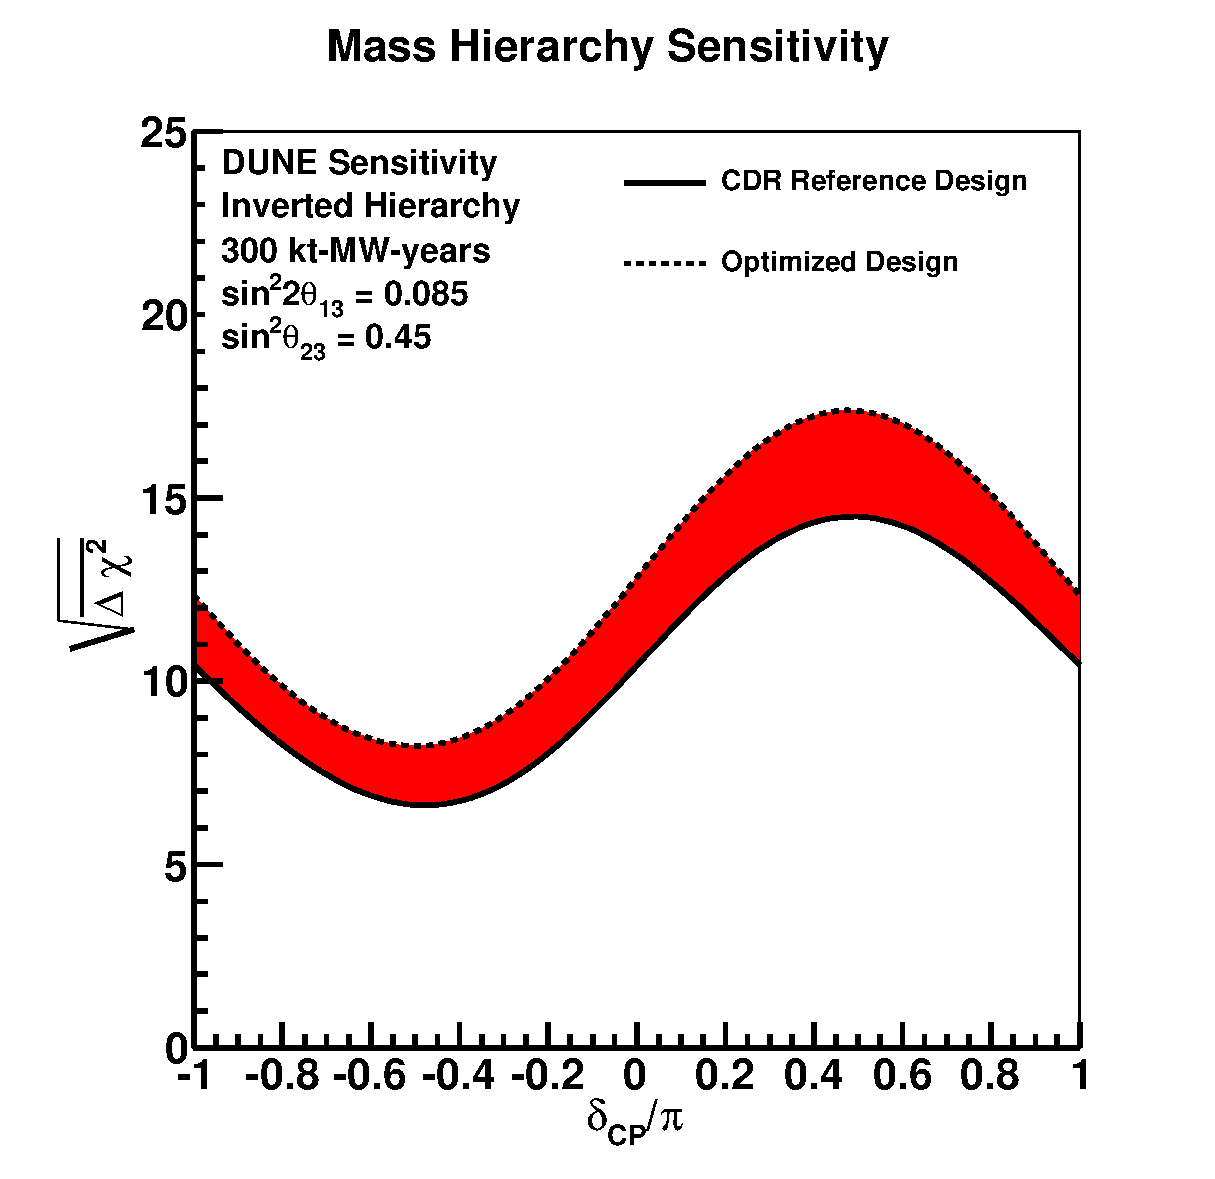
\includegraphics[width=0.49\textwidth]{mh_300ktmwyear_ih}
\end{cdrfigure}

\begin{cdrfigure}[Mass hierarchy sensitivity as a function of exposure]{mh_exposure}{The minimum significance with which the mass hierarchy can be determined for all values of \deltacp as a function of exposure.  The shaded region represents the range in sensitivity due to potential variations in the beam design. This plot assumes normal mass hierarchy. (The inverted hierarchy case is very similar.)}
 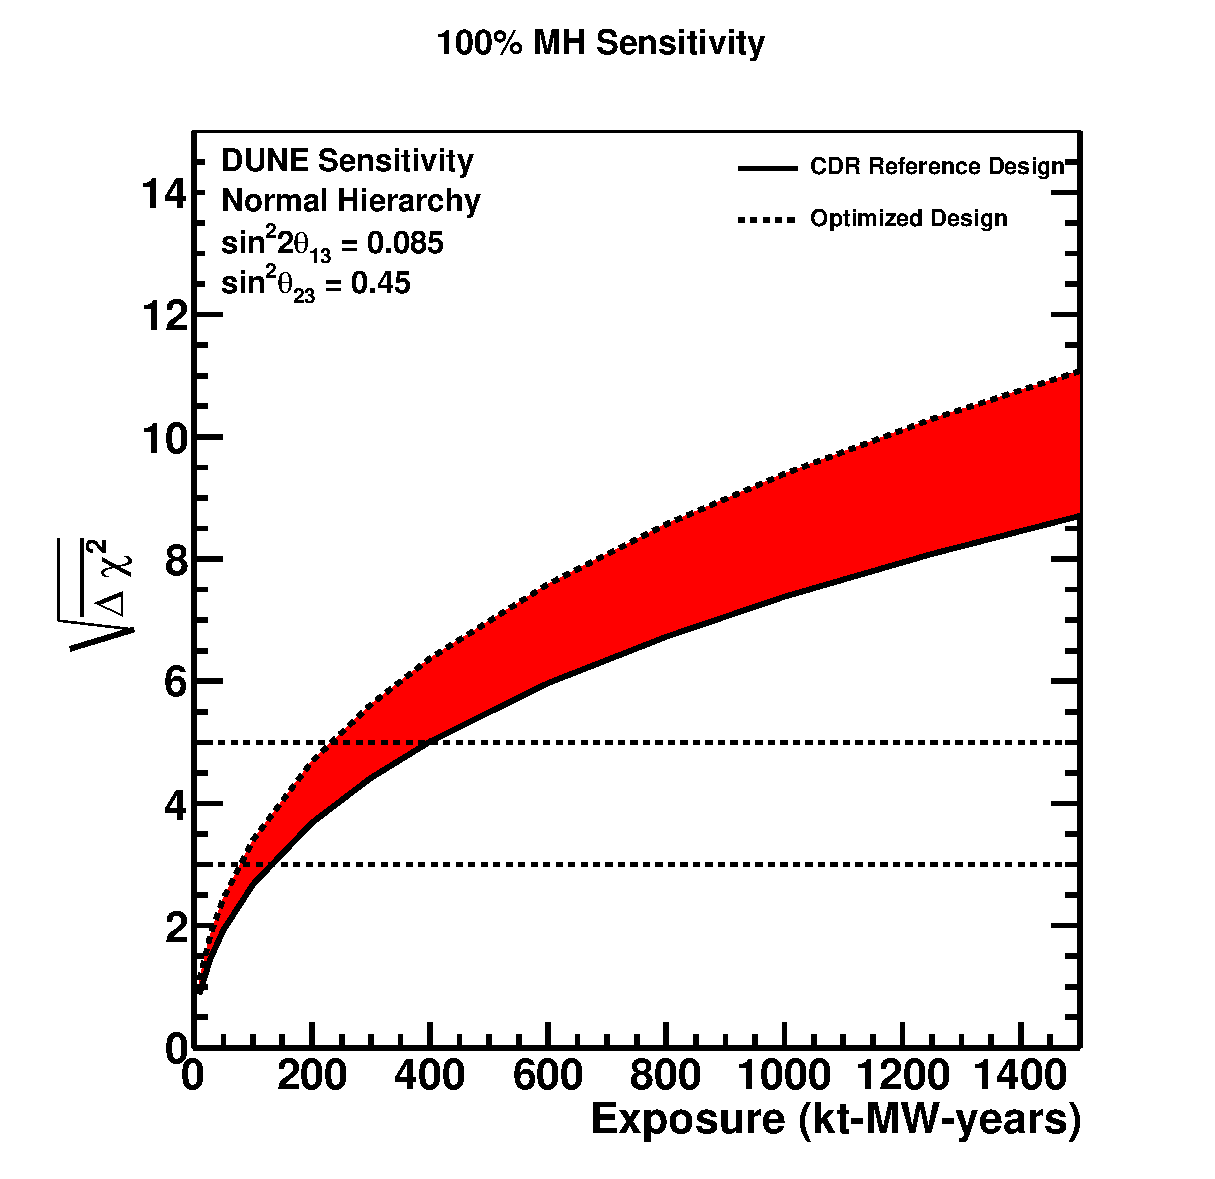
\includegraphics[width=0.7\textwidth]{mh_exp}
\end{cdrfigure}
% \fixme{We are considering an update to Fig~\ref{fig:mh_exposure} where we show CP coverage at 5sigma as a function of exposure, instead of the significance for a fixed CP coverage of 100\% (which is the current version).}

Figures~\ref{fig:mh_theta23}, \ref{fig:mh_theta13}, and \ref{fig:mh_deltamsq} show the variation in the MH sensitivity due to different values of $\theta_{23}$, $\theta_{13}$, and \dm{31} within the allowed ranges.  The value of $\theta_{23}$ has the biggest impact on the sensitivity, and the least favorable scenario corresponds to a true value of \deltacp in which the MH asymmetry
is maximally offset by the leptonic CP asymmetry, and where, independently, 
$\sin^2{\theta_{23}}$ takes on a value at the low end of its 
experimentally allowed range.

\begin{cdrfigure}[Variation in MH sensitivity due to $\theta_{23}$]{mh_theta23}{The variation in the MH sensitivity due to different values of $\theta_{23}$ within the allowed range.  In this figure, the nominal value of $\sin^2\theta_{23} = 0.45$ provides a significance of at least $\sqrt{\overline{\Delta\chi^{2}}} = 5$ for all values of \deltacp. (See Figure~\ref{fig:mh_exposure} for the possible range of exposures to achieve this level of significance.) The significance decreases for all values of \deltacp as $\sin^2\theta_{23}$ gets smaller.}
 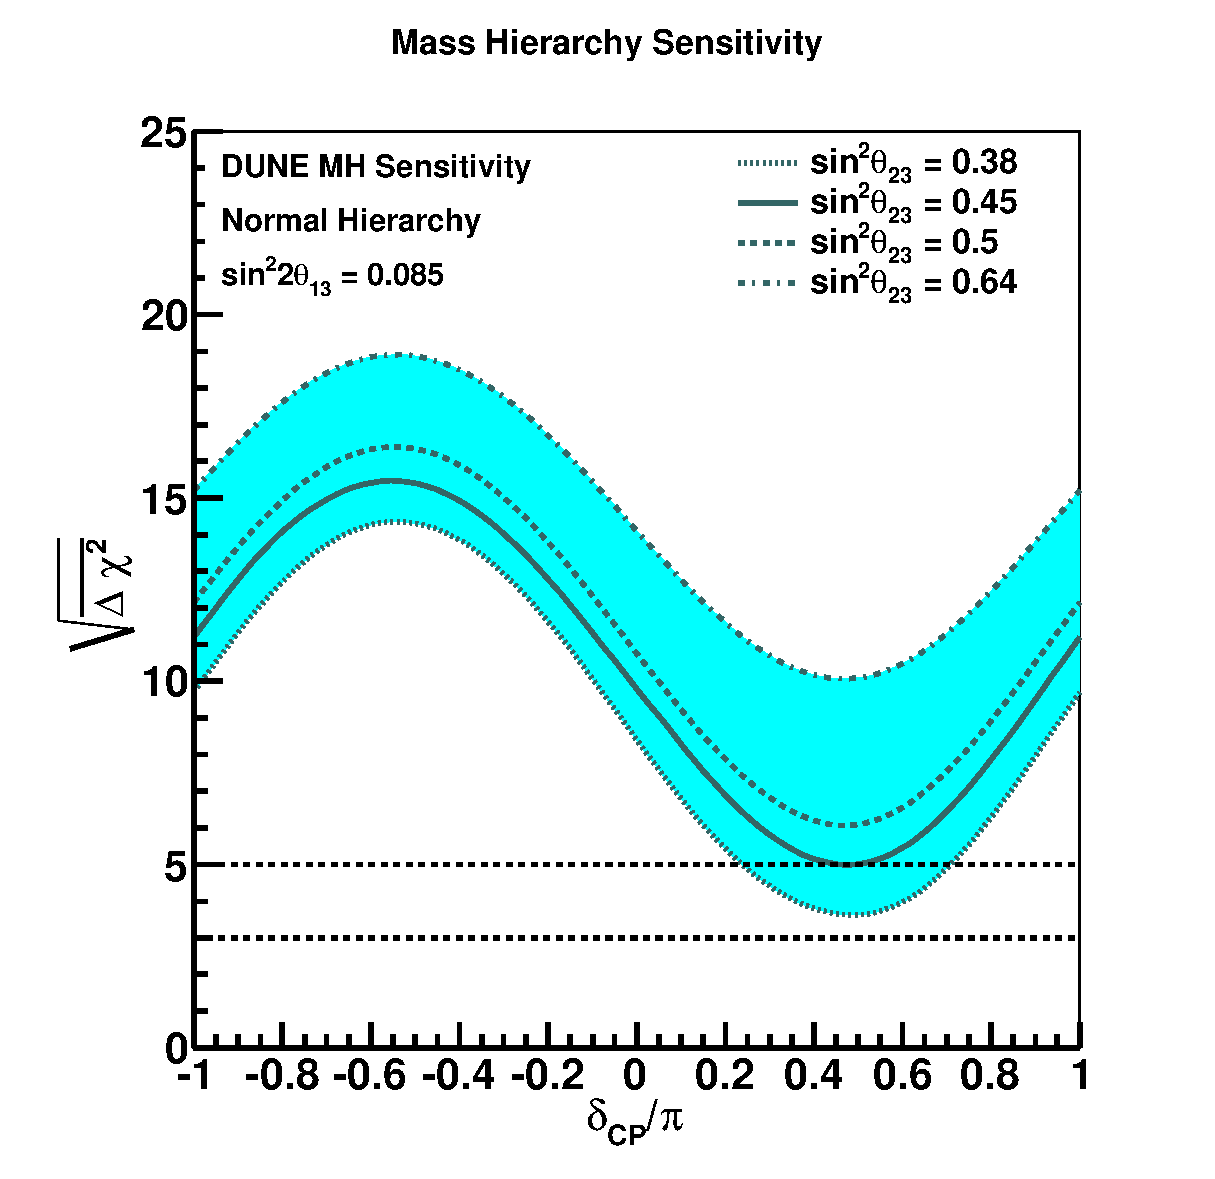
\includegraphics[width=0.7\textwidth]{mh_230ktmwyear_varyth23}
\end{cdrfigure}

\begin{cdrfigure}[Variation in MH sensitivity due to $\theta_{13}$]{mh_theta13}{The variation in the MH sensitivity due to different values of $\theta_{13}$ within the allowed range.  In this figure, he nominal value of $\sin^22\theta_{13} = 0.085$ provides a significance of at least $\sqrt{\overline{\Delta\chi^{2}}} = 5$ for all values of \deltacp.  (See Figure~\ref{fig:mh_exposure} for the possible range of exposures to achieve this level of significance.)}
 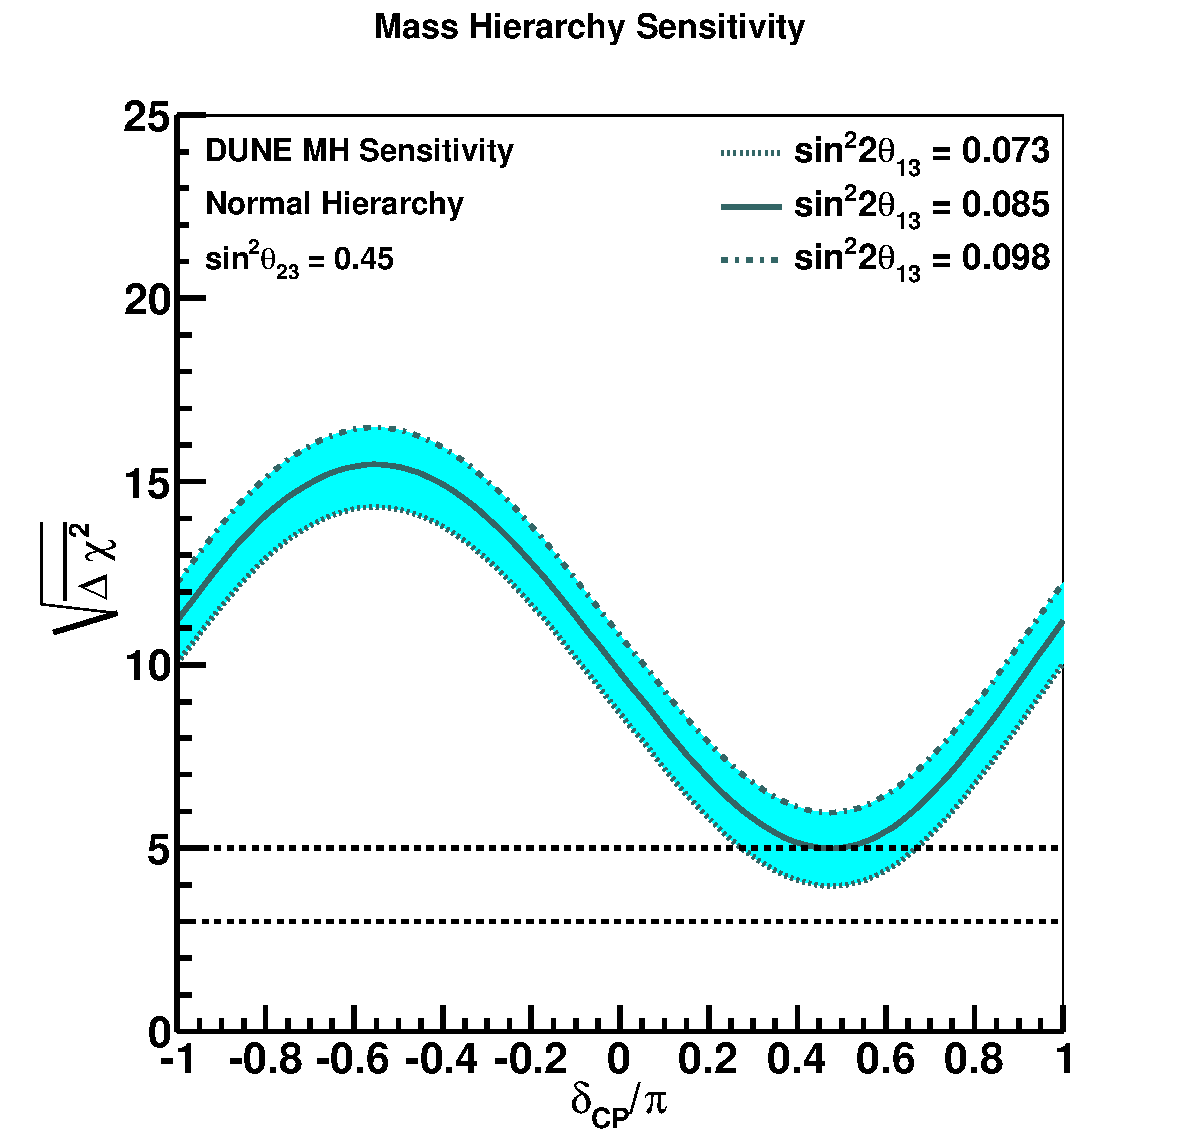
\includegraphics[width=0.7\textwidth]{mh_230ktmwyear_varyth13}
\end{cdrfigure}

\begin{cdrfigure}[Variation in MH sensitivity due to $\Delta m^{2}_{31}$]{mh_deltamsq}{The variation in the MH sensitivity due to different values of \dm{31} within the allowed range.  In this figure, the nominal value of \dm{31} = $2.46\times 10^{-3}$~eV$^2$ provides a significance of at least $\sqrt{\overline{\Delta\chi^{2}}} = 5$ for all values of \deltacp.  (See Figure~\ref{fig:mh_exposure} for the possible range of exposures to achieve this level of significance.)}
 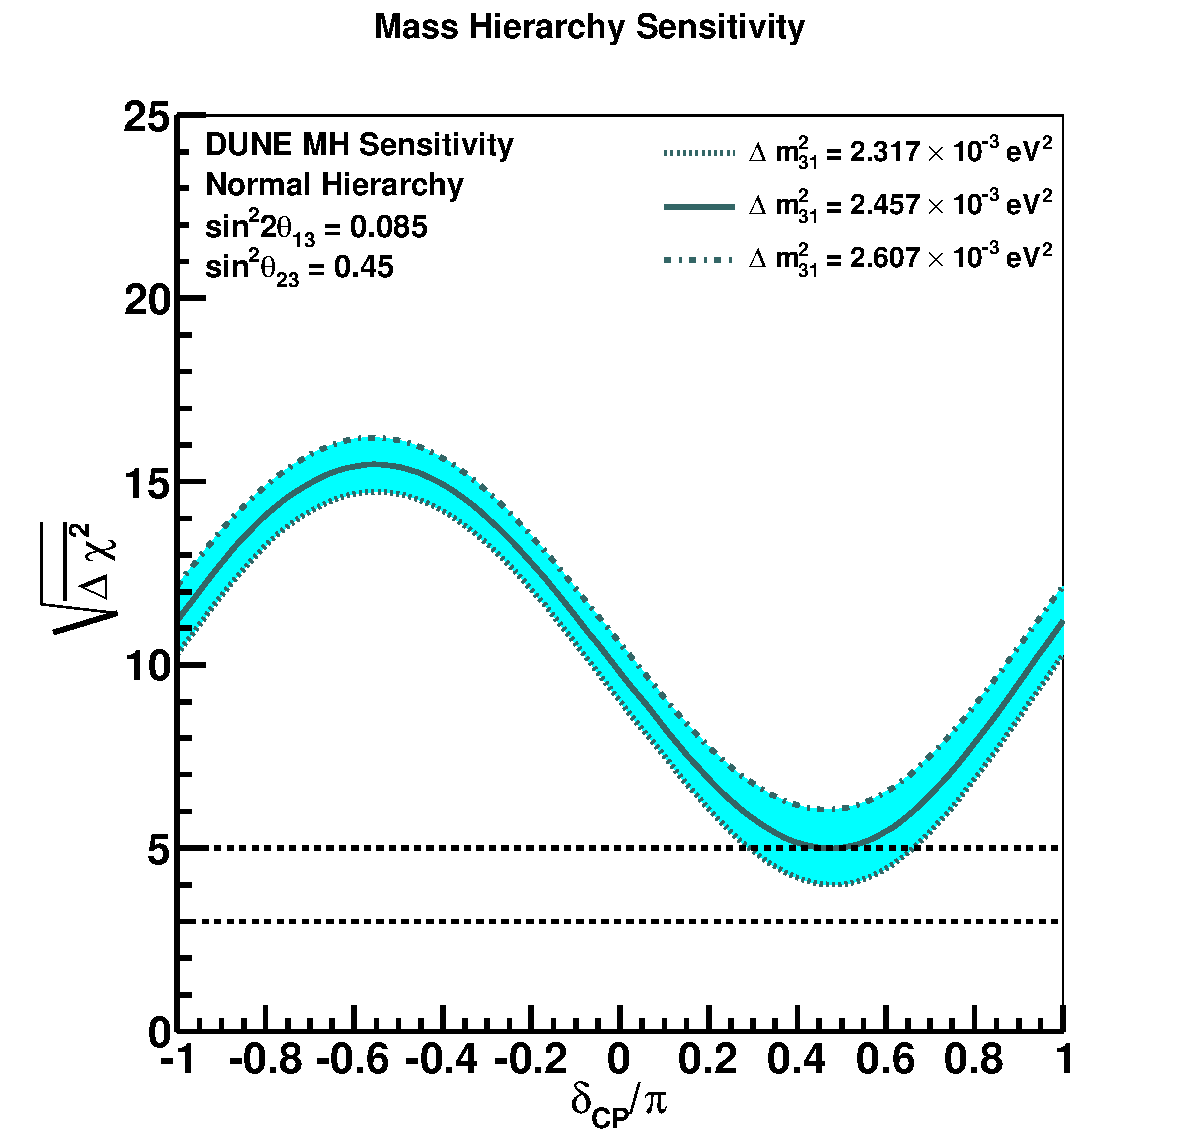
\includegraphics[width=0.7\textwidth]{mh_230ktmwyear_varydmsq}
\end{cdrfigure}
 
Studies have indicated that special attention must be paid to the statistical interpretation of MH sensitivities~\cite{Qian:2012zn,Blennow:2013oma}.
In general, if an experiment is repeated many times, a distribution of $\Delta\chi^2$
values will appear due to statistical fluctuations.
It is usually assumed that the $\Delta \chi^2$ metric follows the expected chi-squared
function for one degree of freedom, which has a mean of
$\overline{\Delta\chi^2}$ and can be interpreted using a Gaussian
distribution with a standard deviation of
$\sqrt{|\overline{\Delta\chi^2}|}$.
In assessing the MH sensitivity of future experiments, it is common practice to generate
a simulated data set (for an assumed true MH) that does not include statistical fluctuations. 
In this typical case, $\overline{\Delta\chi^2}$ is reported as the expected sensitivity, 
where $\overline{\Delta\chi^2}$ is representative of the mean value of $\Delta\chi^2$ that 
would be obtained in an ensemble of experiments for a particular true MH.  
With the exception of Figure~\ref{fig:mhstats}, the sensitivity plots
in this document have been generated using this method.
However, studies in~\cite{Qian:2012zn,Blennow:2013oma}
show that, in the case of the mass hierarchy
determination, the $\Delta \chi^2$ metric {\em does not} follow the expected chi-squared
function for one degree of freedom.  Rather, these studies show that
when the observed counts in the experiment are large enough,
the distribution of $\Delta\chi^2$ used here approximately follows
a Gaussian distribution with a
mean and standard deviation of $\overline{\Delta\chi^2}$ and
$2\sqrt{|\overline{\Delta\chi^2}|}$, respectively. Because the distribution is atypical, the interpretation of 
test statistic values in terms of confidence intervals is different than the standard case.

The effect of statistical fluctuations in the MH measurement is shown in Figure~\ref{fig:mhstats}.  The colored bands show
the possible range in the significance of a MH determination when statistical
fluctuations are included for a measurement that would yield a significance of $\sqrt{\overline{\Delta\chi^{2}}} = 5$
for 100\% of \deltacp values in our standard treatment (the solid blue line).  Also shown in 
Figure~\ref{fig:mhstats} are horizontal lines that specify the confidence level of an experiment that measures a particular
value of $\sqrt{\Delta \chi^2}$, following the convention in~\cite{Qian:2012zn}. An experiment that measures
$\sqrt{\Delta \chi^2} = 5$ (black dashed line) has a $1 - 3.7\times10^{-6}$ probability of determining the
correct MH, while an experiment that measures$\sqrt{\Delta \chi^2} = 3$ (blue dashed line) has a 98.9\% 
probability of determining the correct MH. An experiment that measures $\sqrt{\Delta \chi^2} = 0$ (cyan dashed line)
has a 50\% probability of determining the correct MH.  In this case, both hypotheses (normal or inverted hierarchy) 
fit the data equally well, and the probability of guessing correctly is 50\%.

\begin{cdrfigure}[MH sensitivity including statistical fluctuations]{mhstats}{
  The  sensitivity, given by  $\sqrt{\Delta T}=\sqrt{\Delta\chi^2}$, for a typical experiment 
  (solid blue line) is compared to the bands within which
  68\% (green) and 95\% (yellow) of experiments are expected to fall due to statistical fluctuations.
  The solid blue line (representing a minimum significance of $\sqrt{\Delta T} = 5$ for 100\% of \deltacp
   values) is the expected sensitivity in our standard treatment.
   (See Figure~\ref{fig:mh_exposure} for the possible range of exposures to achieve this level of significance.) 
  The dashed lines show the values of the $\sqrt{\Delta T}$ metric an experiment must measure for the probability of determining
  the correct neutrino MH to be 50\%~(cyan), 98.9\%~(blue), or $(1 - 3.7\times10^{-6})$~(black), following the convention in~\cite{Qian:2012zn}.  
  In the legend, the numbers corresponding to the dashed lines indicate 
  [probability of determining MH {\em incorrectly}] vs. [probability of determining the MH {\em correctly}].}
 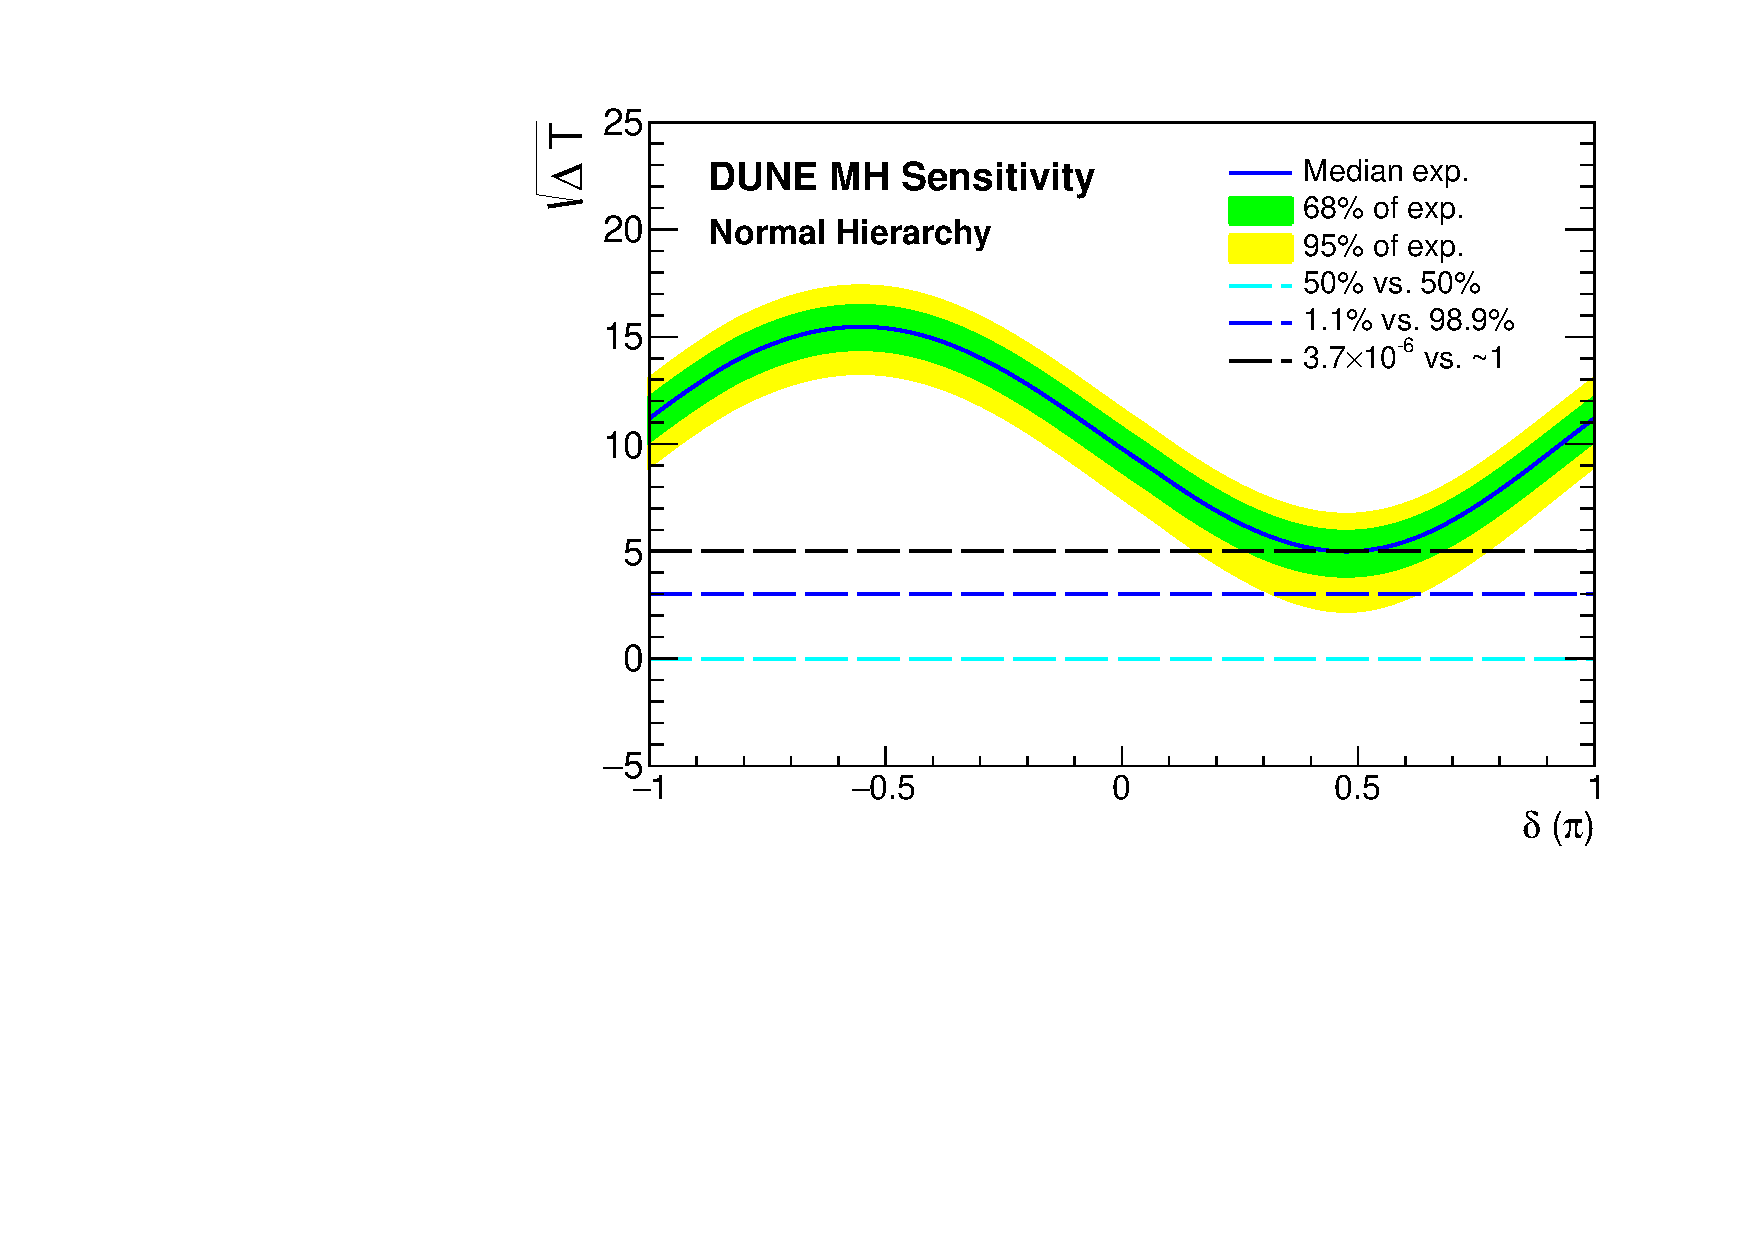
\includegraphics[width=0.7\linewidth]{mhstats_230ktmwyear}
\end{cdrfigure}

The 40-kt DUNE far detector (FD) will be built in 10-kt modules, which will come online over the course of several years.  The near detector (ND) will likely start operations after FD operations are already ongoing.  Without any ND constraints, systematic uncertainties will be larger in the early stages of the experiment. Additionally, the beam power is expected to be upgraded from $\sim$1~MW to $\sim$2~MW during the course of the experiment. For a rough estimate of the sensitivity of DUNE as a function of real time for the first 10~years of operation, we consider the following staging plan:
\begin{itemize}
 \item Year 1: 10~kt FD mass; 1.07~MW beam power; No ND constraints (assume 5\% signal systematic)
 \item Year 2: Add second 10~kt FD module, for a total FD mass of 20~kt
 \item Year 3: Add third 10~kt FD module, for a total FD mass of 30~kt; Include constraints from preliminary ND data analysis (assume 3\% signal systematic)
 \item Year 4: Add fourth 10~kt FD module, for a total FD mass of 40~kt
 \item Year 5: Include constraints from a full ND data analysis (assume 2\% signal systematic)
 \item Year 7: Upgrade of beam power to 2.14~MW
\end{itemize}
We assume previous data sets can be reanalyzed with new assumptions, so each improvement in systematic uncertainty is applied to the full exposure up to that point.  Figure~\ref{fig:mh_staging} shows the MH sensitivity as a function of time considering this very preliminary staging plan.
%Add that integrated exposure is 535 kt-MW-yr after 10 years?

\begin{cdrfigure}[Mass hierarchy sensitivity over time]{mh_staging}{The MH sensitivity as a function of time, including expected increases in FD detector mass, ND constraints on systematic uncertainties, and beam power over time.  The beginning time is defined as the time when the first FD module records neutrinos from LBNF.  The shaded region represents the range in sensitivity due to potential variations in the beam design.  The staging plan shown here is very preliminary.}
 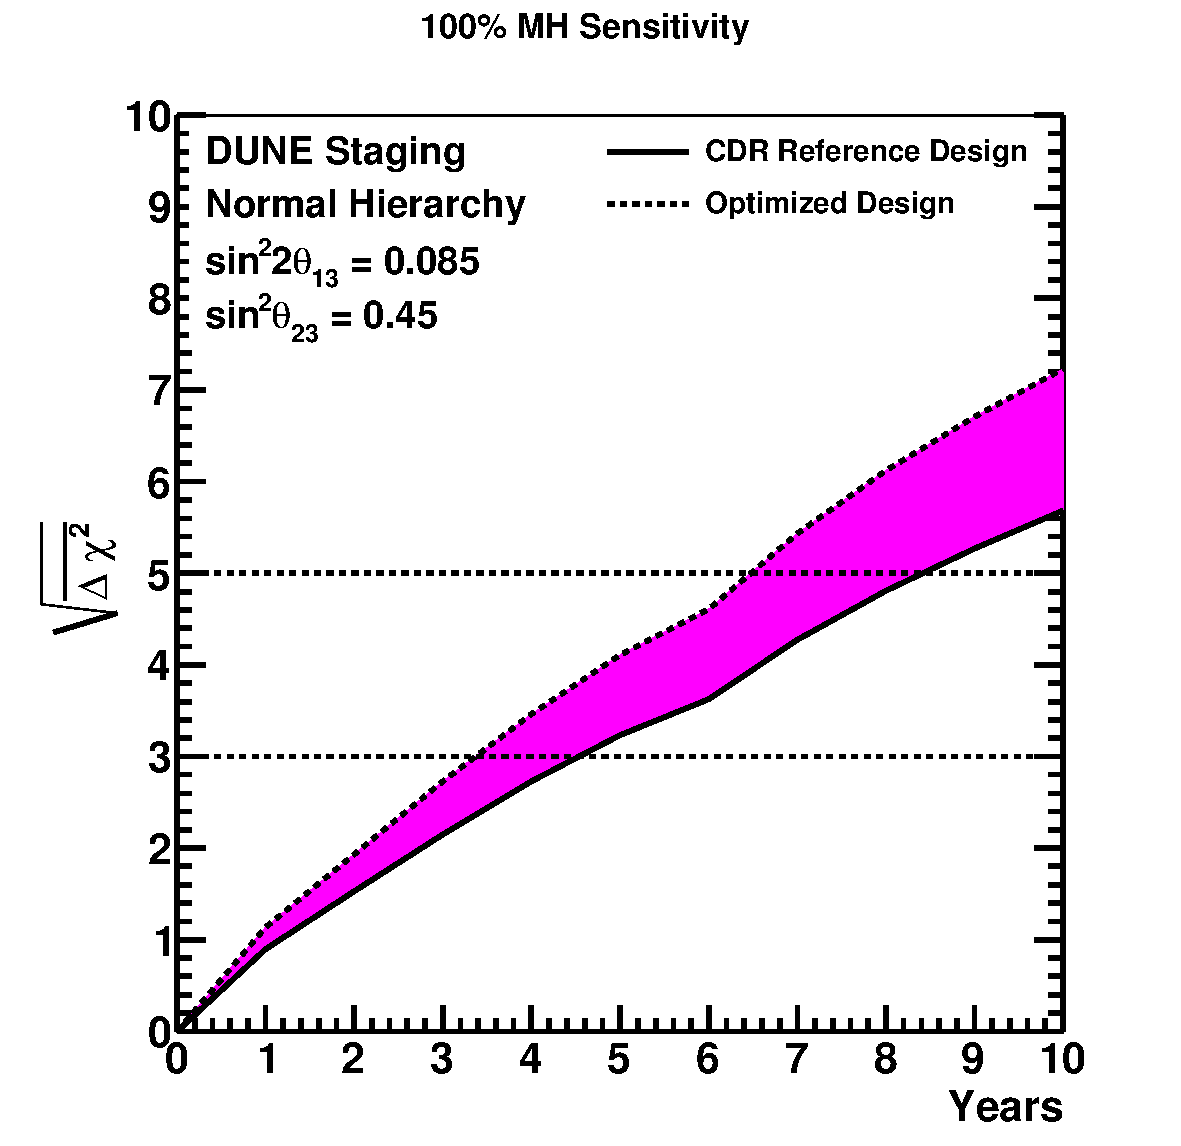
\includegraphics[width=0.7\textwidth]{mh_exp_staging}
\end{cdrfigure}


\section{CP-symmetry Violation}
\label{sec:physics-lbnosc-cpv}

In the particular parameterization of the PMNS matrix shown in
Equation~\ref{eqn:pmns}, the middle factor, labeled `II', describes
the mixing between the $\nu_1$ and $\nu_3$ mass states, and depends on
the CP-violating phase \deltacp.  With the recent measurement of $\theta_{13}$, we now know
that the conditions for measuring \deltacp in the three-flavor framework 
have been met; all three mixing angles are nonzero, and there are two distinct mass splittings.
In the approximation for the electron neutrino appearance probability given in Equation~\ref{eqn:appprob}, 
expanding the middle term results in the presence of CP-odd terms (dependant on $\sin \mdeltacp$) that have opposite signs 
in $\nu_{\mu} \rightarrow \nu_e$ and $\overline{\nu}_{\mu} \rightarrow \overline{\nu}_e$ oscillations.
For $\mdeltacp \neq 0$ or $\pi$, these terms introduce an
asymmetry in neutrino versus antineutrino oscillations. The magnitude of the
CP-violating terms in the oscillation depends most directly on the size of 
the Jarlskog Invariant~\cite{Jarlskog:1985cw}, a function that was
introduced to provide a measure of CP violation independent of the 
mixing-matrix parameterization. In terms of the parameterization presented in Equation~\ref{eqn:pmns},
the Jarlskog Invariant is:
%
\begin{equation}
J_{CP}^{\rm PMNS} \equiv \frac{1}{8} \sin 2 \theta_{12} \sin 2 \theta_{13}
\sin 2 \theta_{23} \cos \theta_{13} \sin \mdeltacp.
\end{equation}
The relatively large values of the mixing angles in the lepton sector imply that
leptonic CP-violation effects may be quite large ---  
depending on the value of the phase \deltacp, which is currently unknown. 
Experimentally, it is unconstrained at the 3$\sigma$ level by the global fit~\cite{Gonzalez-Garcia:2014bfa}.
Given the current best-fit values of the mixing angles~\cite{Gonzalez-Garcia:2014bfa} and assuming normal hierarchy,
\begin{equation}
J_{CP}^{\rm PMNS} \approx 0.03 \sin \mdeltacp.
\end{equation}
This is in sharp contrast to the very small mixing in the quark sector,  
which leads to a very small value of the corresponding quark-sector
Jarlskog Invariant~\cite{Beringer:1900zz},
\begin{equation}
J_{CP}^{\rm CKM} \approx 3 \times 10^{-5},
\end{equation}
despite the large value of $\delta^{\rm CKM}_{CP}\approx70^{\circ}$.

The variation in the $\nu_\mu \rightarrow
\nu_e$ oscillation probability (Equation~\ref{eqn:appprob}) with the value of \deltacp
indicates that it is experimentally possible to measure the value of
\deltacp at a fixed baseline using only the observed shape of the
$\nu_\mu \rightarrow \nu_e$ {\em or} the 
$\overline{\nu}_\mu \rightarrow \overline{\nu}_e$
appearance signal measured over an energy range that encompasses at
least one full oscillation interval. A measurement of the value of
$\mdeltacp \neq 0 \ {\rm or} \ \pi$, assuming that neutrino mixing follows the three-flavor model, would imply CP violation.  

The CP asymmetry,
$\mathcal{A}_{CP}$, is defined as 
\begin{equation}
\label{eqn:cp-asymm}
 \mathcal{A}_{CP} = \frac{P(\nu_\mu \rightarrow \nu_e) -
  P(\overline{\nu}_\mu \rightarrow \overline{\nu}_e)}{P(\nu_\mu \rightarrow
  \nu_e) + P(\overline{\nu}_\mu \rightarrow \overline{\nu}_e)}.
\end{equation}
In the three-flavor model the asymmetry can be approximated to leading
order in $\Delta m_{21}^2$ as~\cite{Marciano:2006uc}:
\begin{equation}
\mathcal{A}_{CP} \sim \frac{\cos \theta_{23} \sin 2 \theta_{12}
  {\sin \mdeltacp}}{\sin \theta_{23} \sin \theta_{13}}
\left(\frac{\Delta m^2_{21} L}{ 4 E_{\nu}}\right) + {\rm matter
  \ effects}
\label{eqn:cpasym}
\end{equation}
Regardless of the measured value obtained for \deltacp, the explicit observation
of the asymmetry $\mathcal{A}_{CP}$ in $\nu_{\mu} \rightarrow \nu_e$ and $\overline{\nu}_{\mu} \rightarrow \overline{\nu}_e$
oscillations is sought to directly demonstrate the
leptonic CP violation effect.  A measurement of \deltacp that is inconsistent with the measurement of $\mathcal{A}_{CP}$
according to Equation~\ref{eqn:cpasym} could be evidence of of physics beyond the standard three-flavor model.
For long-baseline experiments such as DUNE, where the neutrino beam propagates through 
the Earth's mantle, the leptonic CP-violation effects must be disentangled from 
the matter effects.

Figure~\ref{fig:cpv_nominal} shows the significance with which the CP violation ($\mdeltacp \neq 0 \ {\rm or} \ \pi$) can be determined as a function of the value of \deltacp for an exposure of 300~kt-MW-yr, which corresponds to seven years of data (3.5 years in neutrino mode plus 3.5 years in antineutrino mode) with a 40-kt detector and a 1.07-MW beam.  Figure~\ref{fig:cpv_exposure} shows the significance with which CP violation can be determined for 50\% or 75\% of \deltacp values as a function of exposure.  Table~\ref{tab:cpv_requiredexposure} lists the minimum exposure required to determine CP violation with a significance of 5$\sigma$ for 50\% of \deltacp values or 3$\sigma$ for 75\% of \deltacp values for both the CDR reference beam design and the optimized beam design.  The CP violation sensitivity as a function of \deltacp as shown in Figure~\ref{fig:cpv_nominal} has a characteristic double peak structure because the significance of a CP violation measurement necessarily drops to zero where there is no CP violation: at the CP-conserving values of $-\pi,~0,~{\rm and}~\pi$.  Therefore, unlike the MH determination, it's not possible for any experiment to provide 100\% coverage in \deltacp for a CP violation measurement because CP violation effects vanish at certain values of \deltacp.

\begin{cdrfigure}[CP violation sensitivity for a 300~kt-MW-yr exposure]{cpv_nominal}{The significance with which the CP violation can be determined as a function of the value of \deltacp for an exposure of 300~kt-MW-yr assuming normal MH (left) or inverted MH (right).  The shaded region represents the range in sensitivity due to potential variations in the beam design.}
 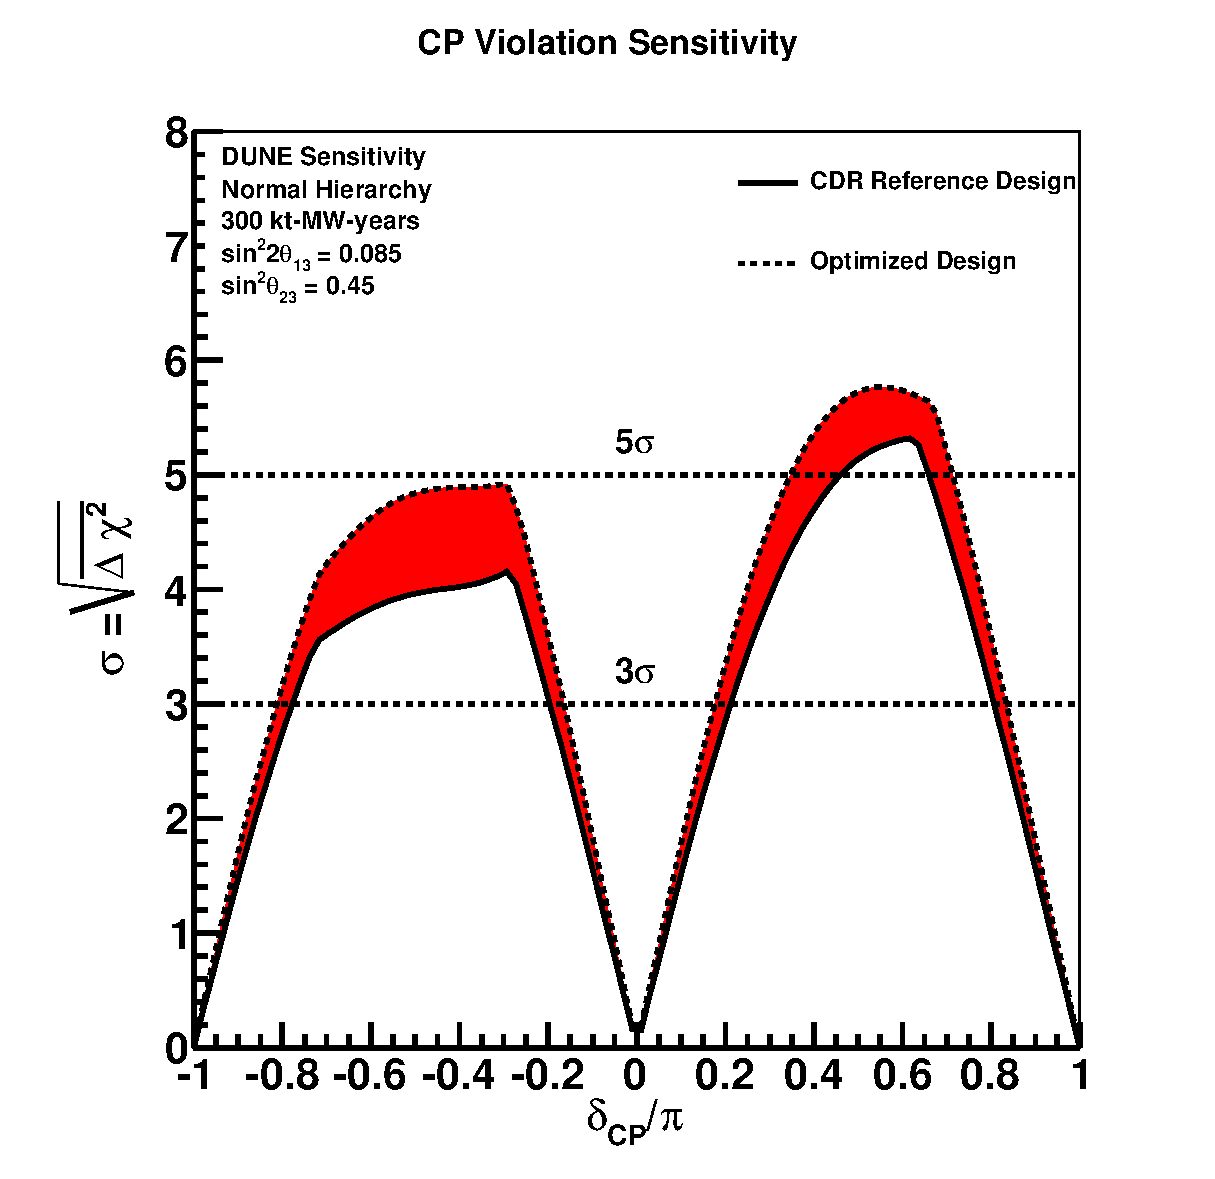
\includegraphics[width=0.49\textwidth]{cpv_300ktmwyear}
 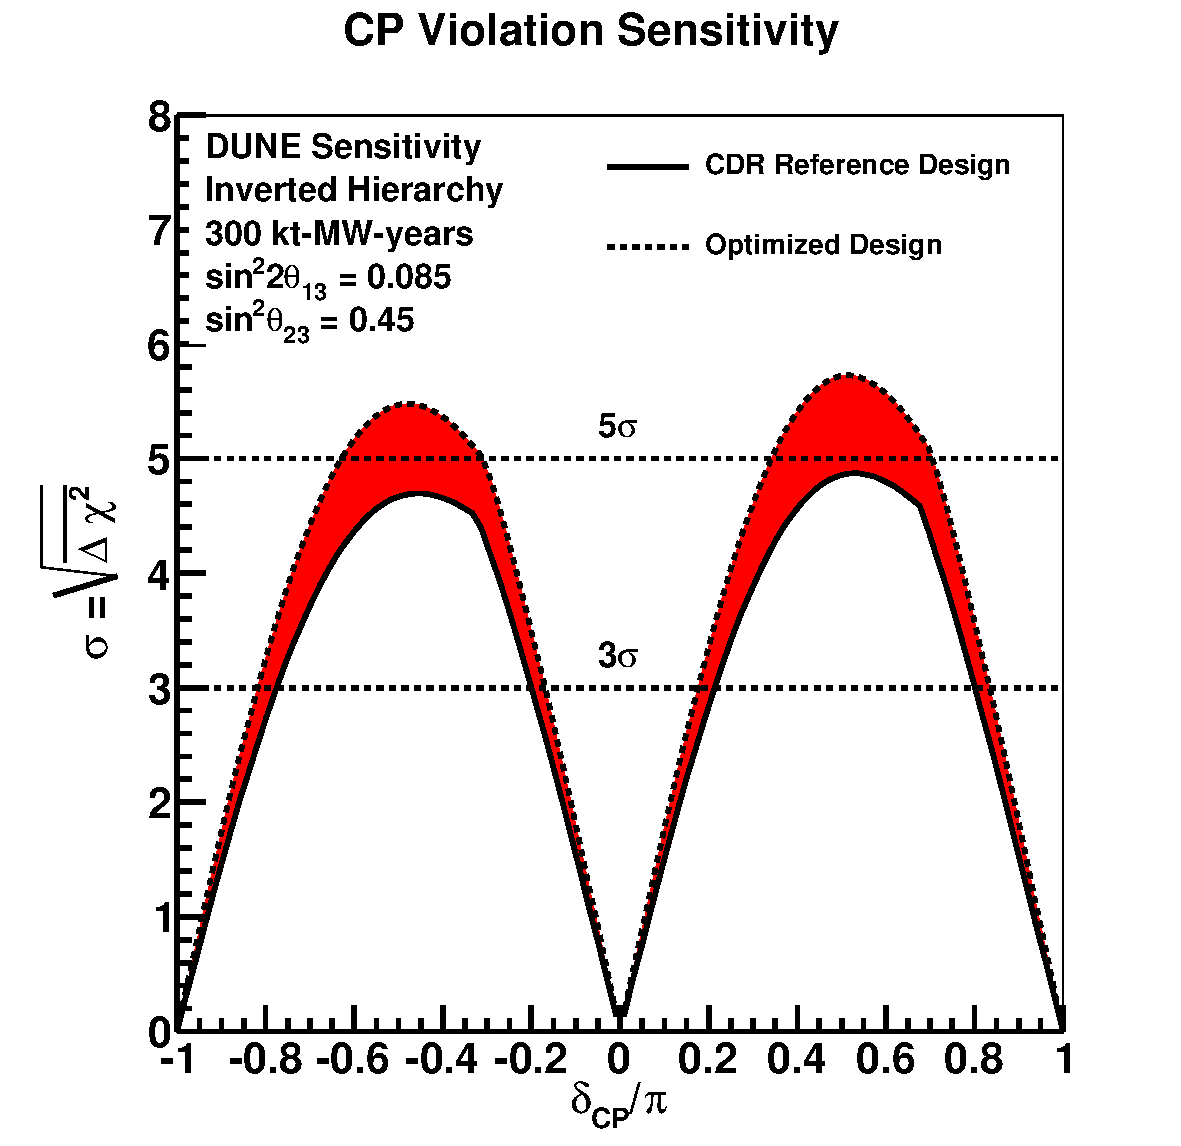
\includegraphics[width=0.49\textwidth]{cpv_300ktmwyear_ih}
\end{cdrfigure}

\begin{cdrfigure}[CP violation sensitivity as a function of exposure]{cpv_exposure}{The significance with which CP violation can be determined for 50\% (left) or 75\% (right) of \deltacp values as a function of exposure.  The shaded region represents the range in sensitivity due to potential variations in the beam design. This plot assumes normal mass hierarchy.}
 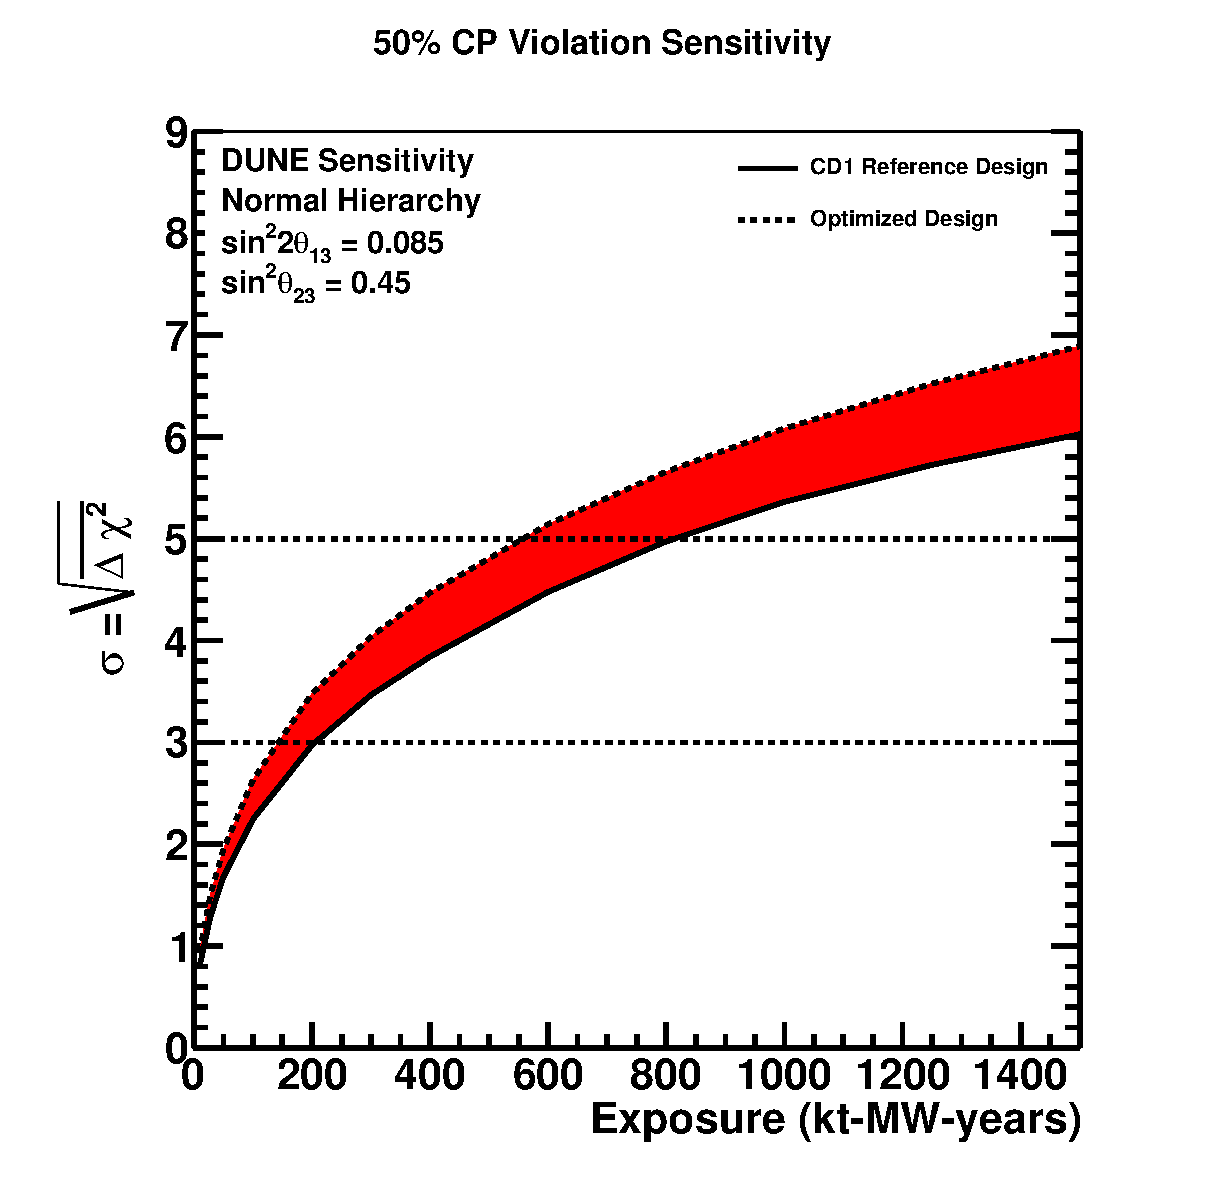
\includegraphics[width=0.49\textwidth]{cpv50_exp}
 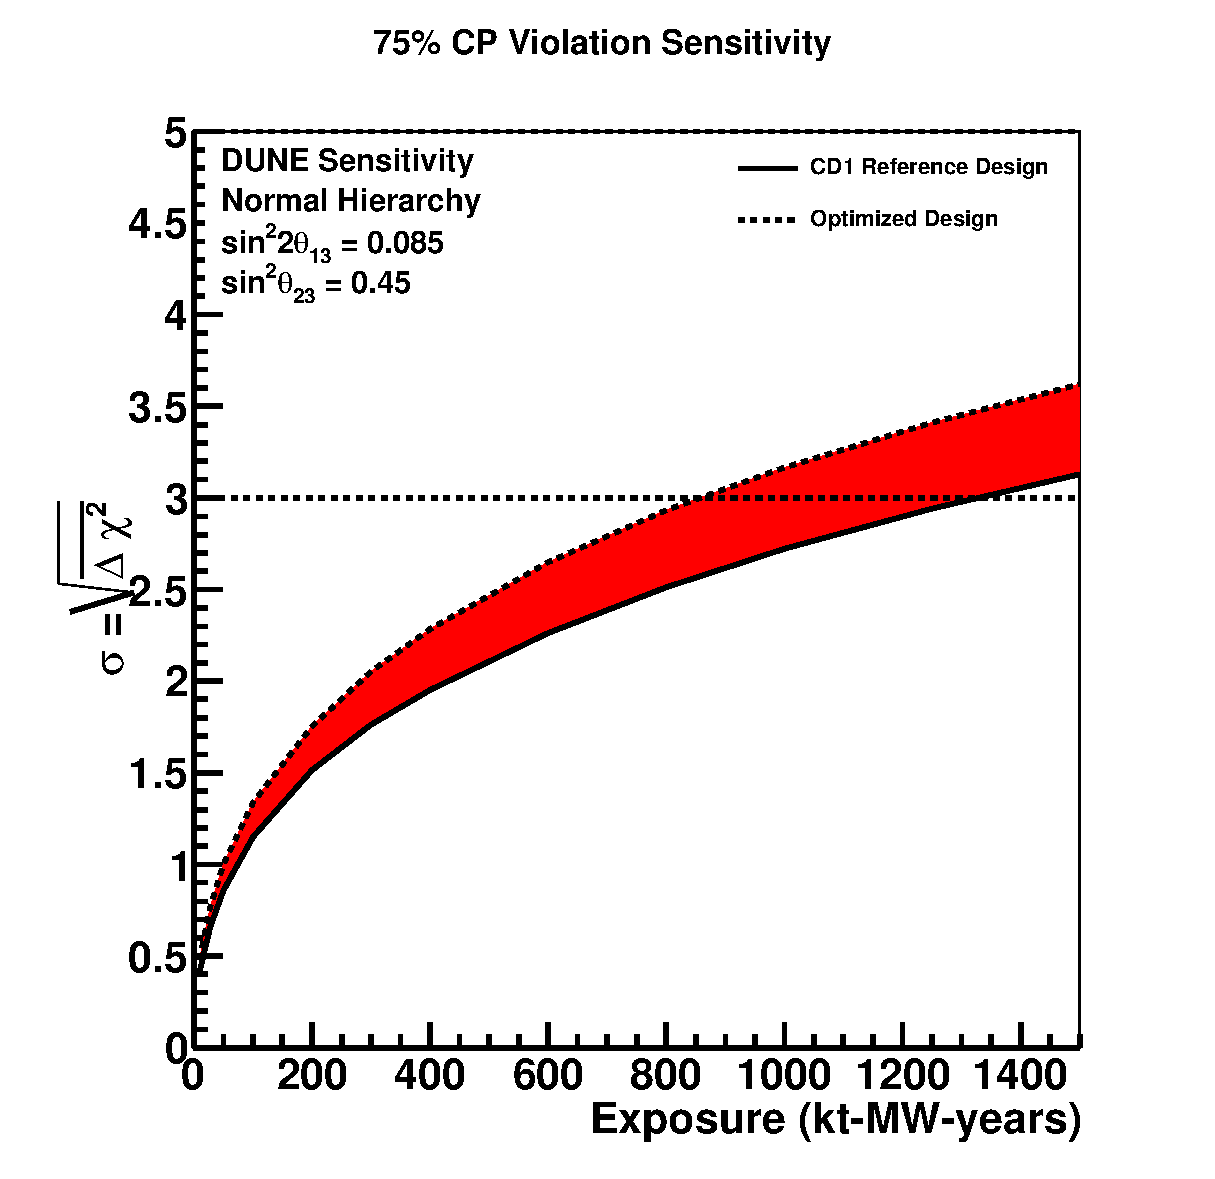
\includegraphics[width=0.49\textwidth]{cpv75_exp}
\end{cdrfigure}
% \fixme{We are considering an update to Fig~\ref{fig:cpv_exposure} where we show CP coverage at 3sigma or 5sigma as a function of exposure, instead of the significance for a fixed CP coverage of 50\% and 75\% (which is the current version).}

\begin{cdrtable}[Required exposure for a CP violation measurement]{lcc}{cpv_requiredexposure}{The minimum exposure required to determine CP violation with a significance of 3$\sigma$ for 75\% of \deltacp values or 5$\sigma$ for 50\% of \deltacp values for the CDR reference beam design and the optimized beam design.}
 Significance & CDR Reference Design & Optimized Design\\
 \toprowrule
 3$\sigma$ for 75\% of \deltacp values & 1300~kt-MW-yr & 850~kt-MW-yr \\
 5$\sigma$ for 50\% of \deltacp values & 550~kt-MW-yr & 800~kt-MW-yr\\
\end{cdrtable}

Figures~\ref{fig:cpv_theta23}, \ref{fig:cpv_theta13}, and \ref{fig:cpv_deltamsq} show the variation in the CP sensitivity due to different values of $\theta_{23}$, $\theta_{13}$, and \dm{31} within the allowed ranges.  The value of $\theta_{23}$ has the biggest impact on the sensitivity, and the least favorable scenario corresponds to a value of $\sin^2{\theta_{23}}$ at the high end of its 
experimentally allowed range.

\begin{cdrfigure}[Variation in CP sensitivity due to $\theta_{23}$]{cpv_theta23}{The variation in the CP sensitivity due to different values of $\theta_{23}$ within the allowed range.  In this figure, the nominal value of $\sin^2\theta_{23} = 0.45$ provides a significance of at least 3$\sigma$ for 75\% of \deltacp values. (See Figure~\ref{fig:cpv_exposure} for the possible range of exposures to achieve this level of significance.) The significance decreases for all values of \deltacp as $\sin^2\theta_{23}$ gets larger.}
 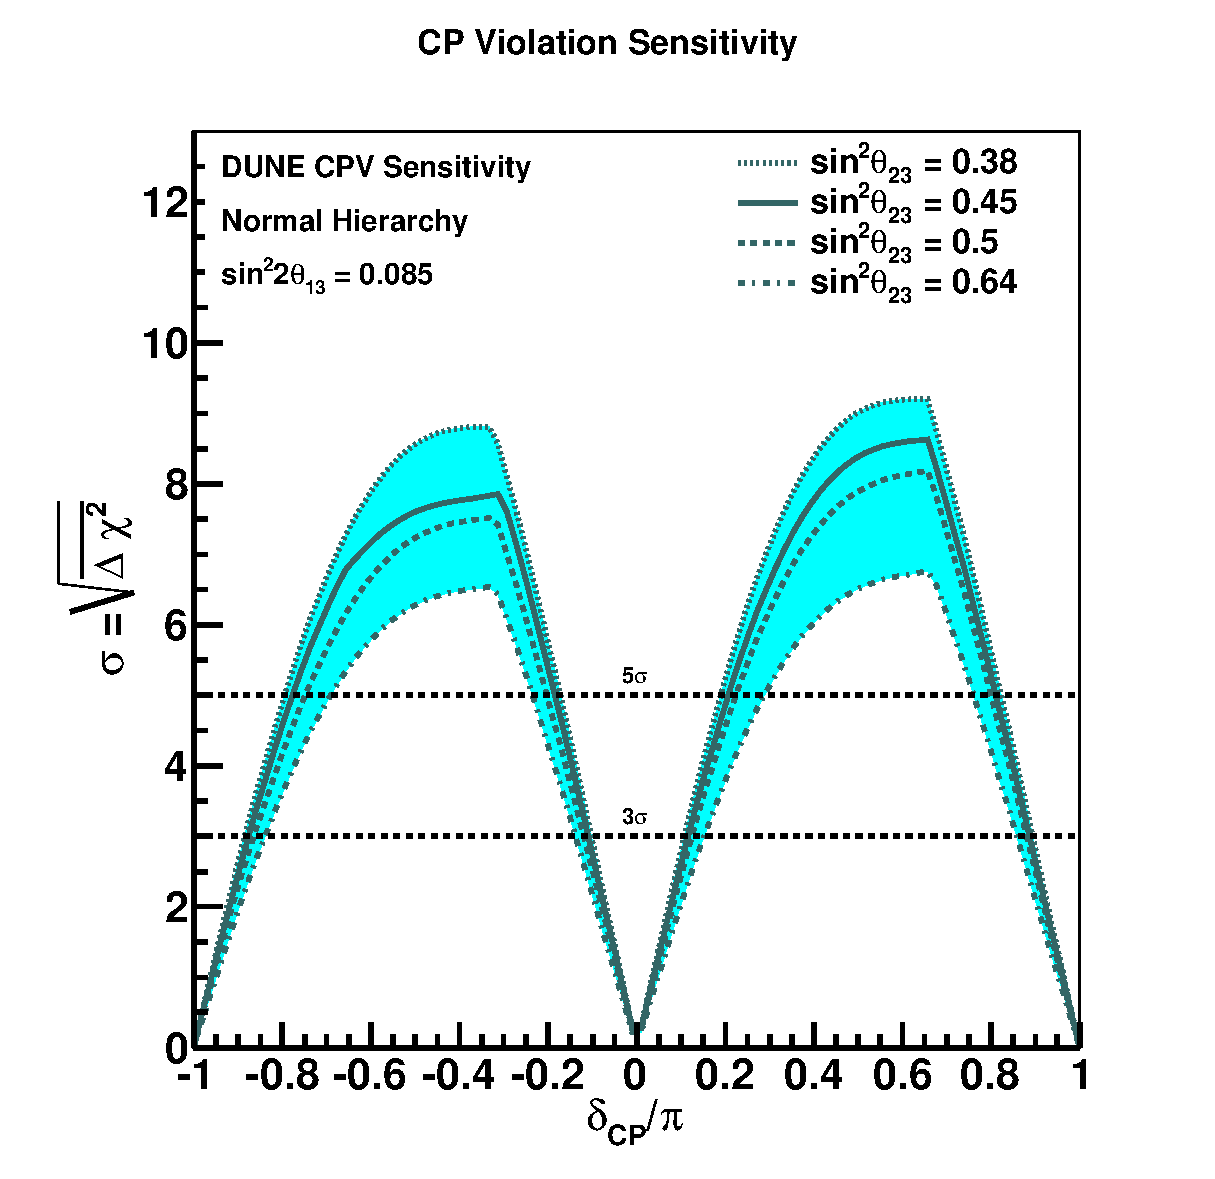
\includegraphics[width=0.7\textwidth]{cpv_890ktmwyear_varyth23}
\end{cdrfigure}

\begin{cdrfigure}[Variation in CP sensitivity due to $\theta_{13}$]{cpv_theta13}{The variation in the CP sensitivity due to different values of $\theta_{13}$ within the allowed range.  In this figure, the nominal value of $\sin^22\theta_{13} = 0.085$ provides a significance of at least 3$\sigma$ for 75\% of \deltacp values. (See Figure~\ref{fig:cpv_exposure} for the possible range of exposures to achieve this level of significance.)}
 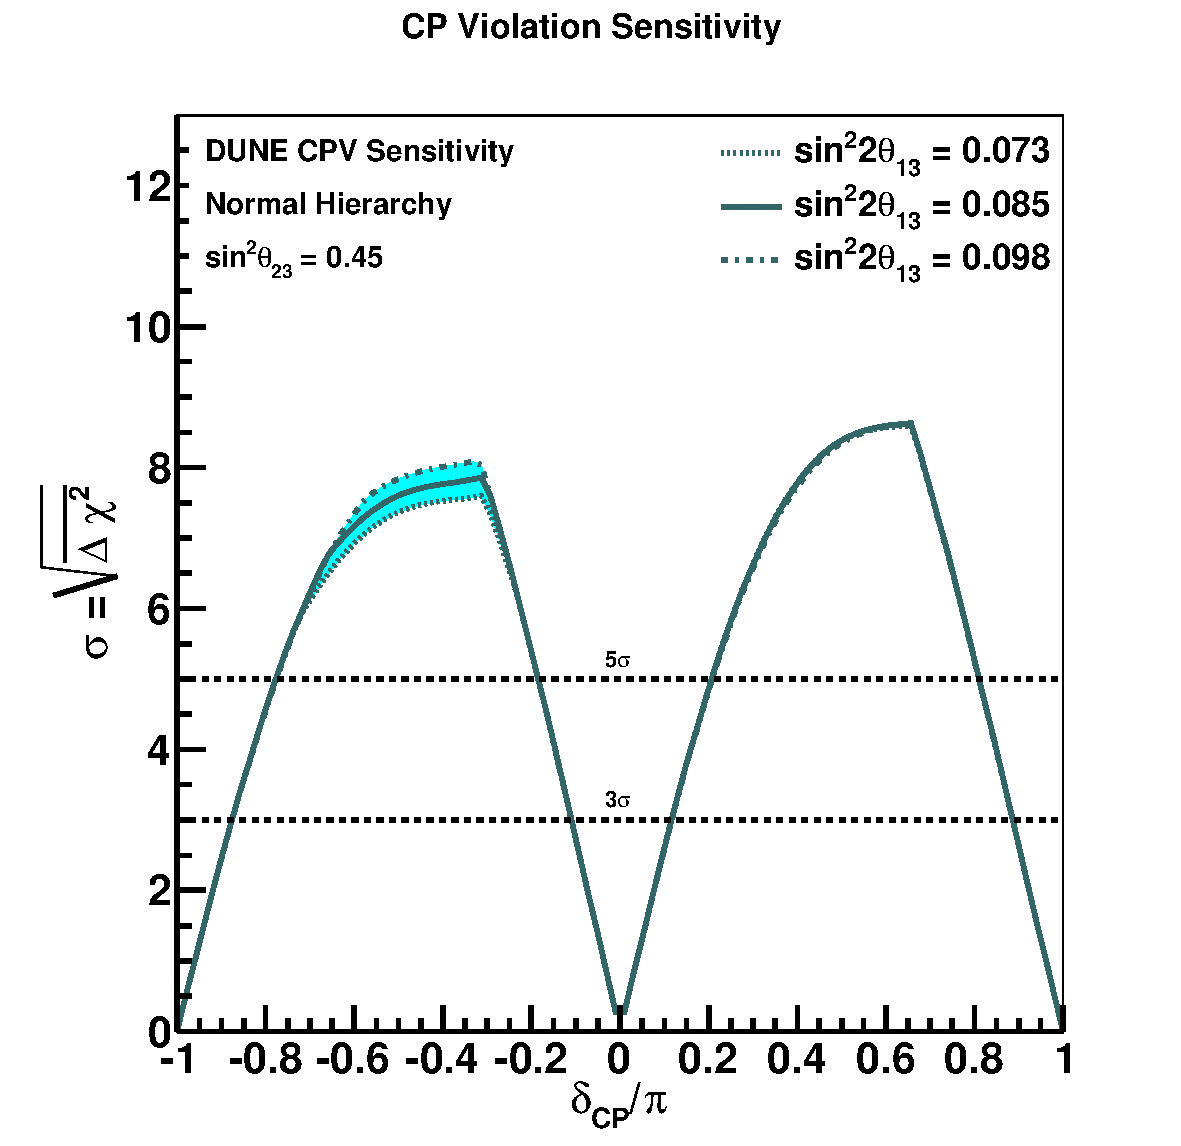
\includegraphics[width=0.7\textwidth]{cpv_890ktmwyear_varyth13}
\end{cdrfigure}

\begin{cdrfigure}[Variation in CP sensitivity due to $\Delta m^{2}_{31}$]{cpv_deltamsq}{The variation in the CP sensitivity due to different values of \dm{31} within the allowed range.  In this figure, the nominal value of \dm{31} = $2.46\times 10^{-3}$~eV$^2$ provides a significance of at least 3$\sigma$ for 75\% of \deltacp values.  (See Figure~\ref{fig:cpv_exposure} for the possible range of exposures to achieve this level of significance.)}
 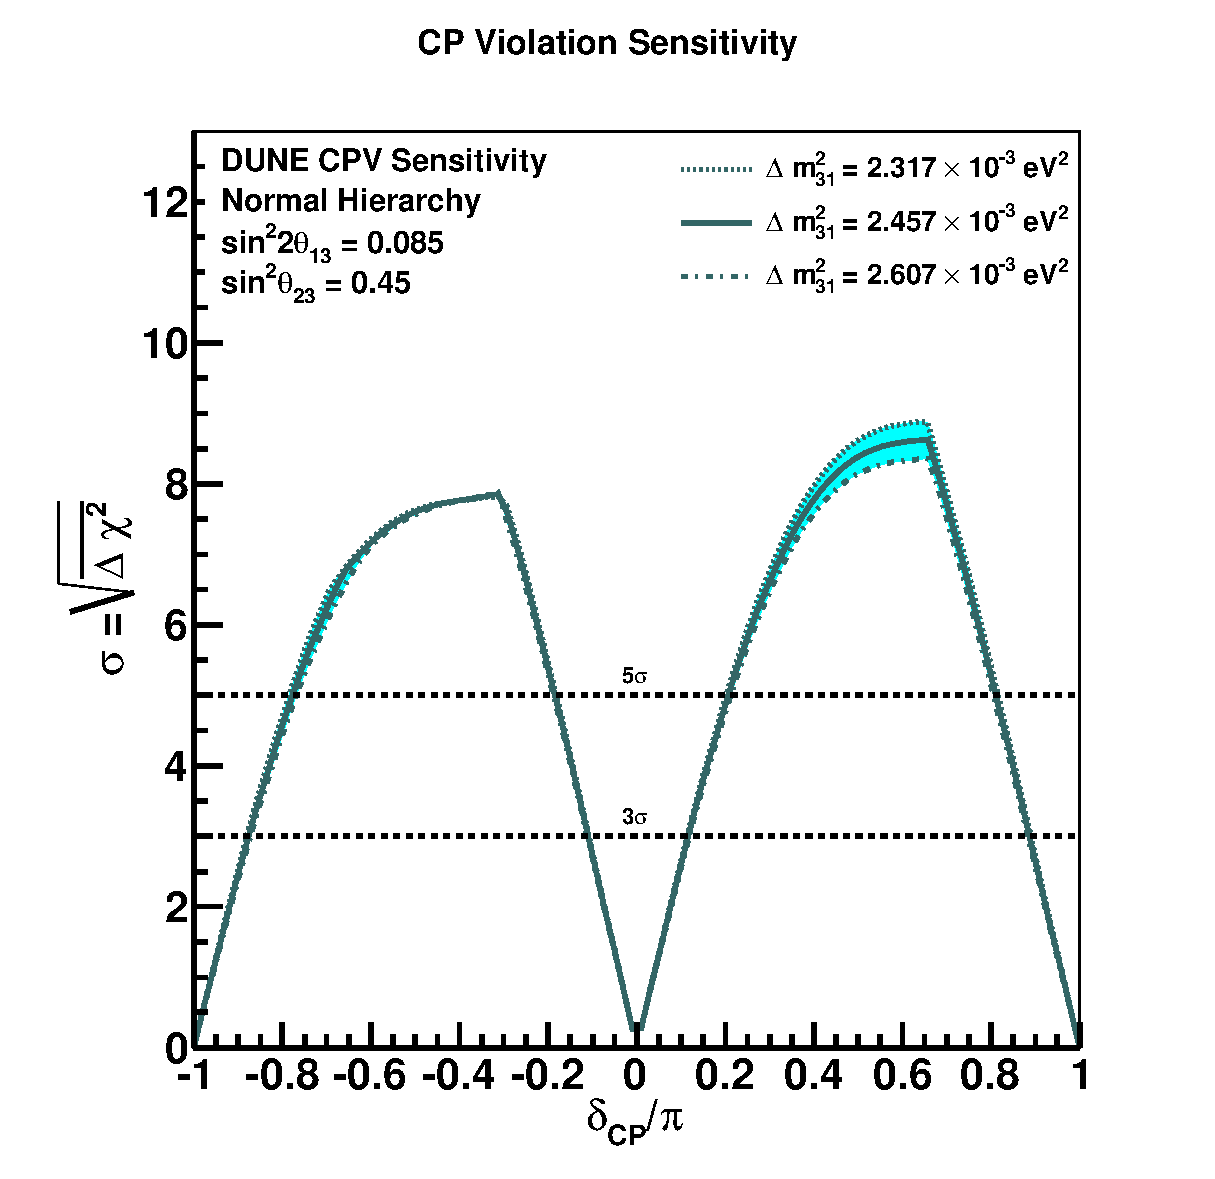
\includegraphics[width=0.7\textwidth]{cpv_890ktmwyear_varydmsq}
\end{cdrfigure}

Figure~\ref{fig:cpv_staging} shows the CP violation sensitivity as a function of time considering the preliminary staging plan presented in Section~\ref{sec:physics-lbnosc-mh}.

\begin{cdrfigure}[CP violation sensitivity over time]{cpv_staging}{The CP violation sensitivity as a function of time, including expected increases in FD detector mass, ND constraints on systematic uncertainties, and beam power over time.  The beginning time is defined as the time when the first FD module records neutrinos from LBNF.  Left: Significance for 50\% coverage of \deltacp values.  Right: Significance for 75\% coverage of \deltacp values.  The shaded region represents the range in sensitivity due to potential variations in the beam design.  The staging plan shown here is very preliminary.}
 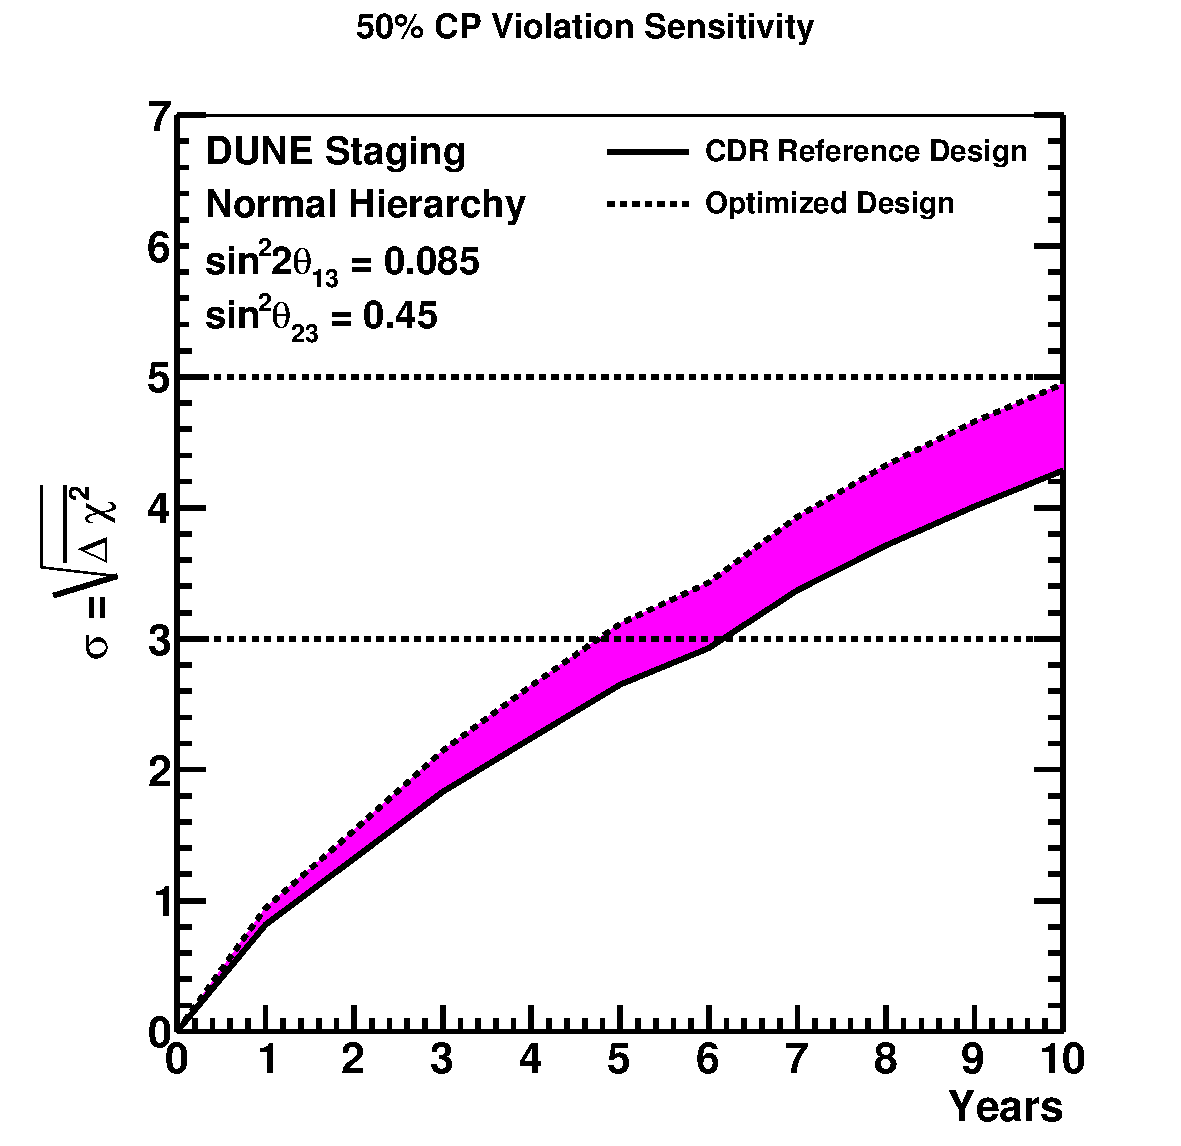
\includegraphics[width=0.49\textwidth]{cpv50_exp_staging.pdf}
 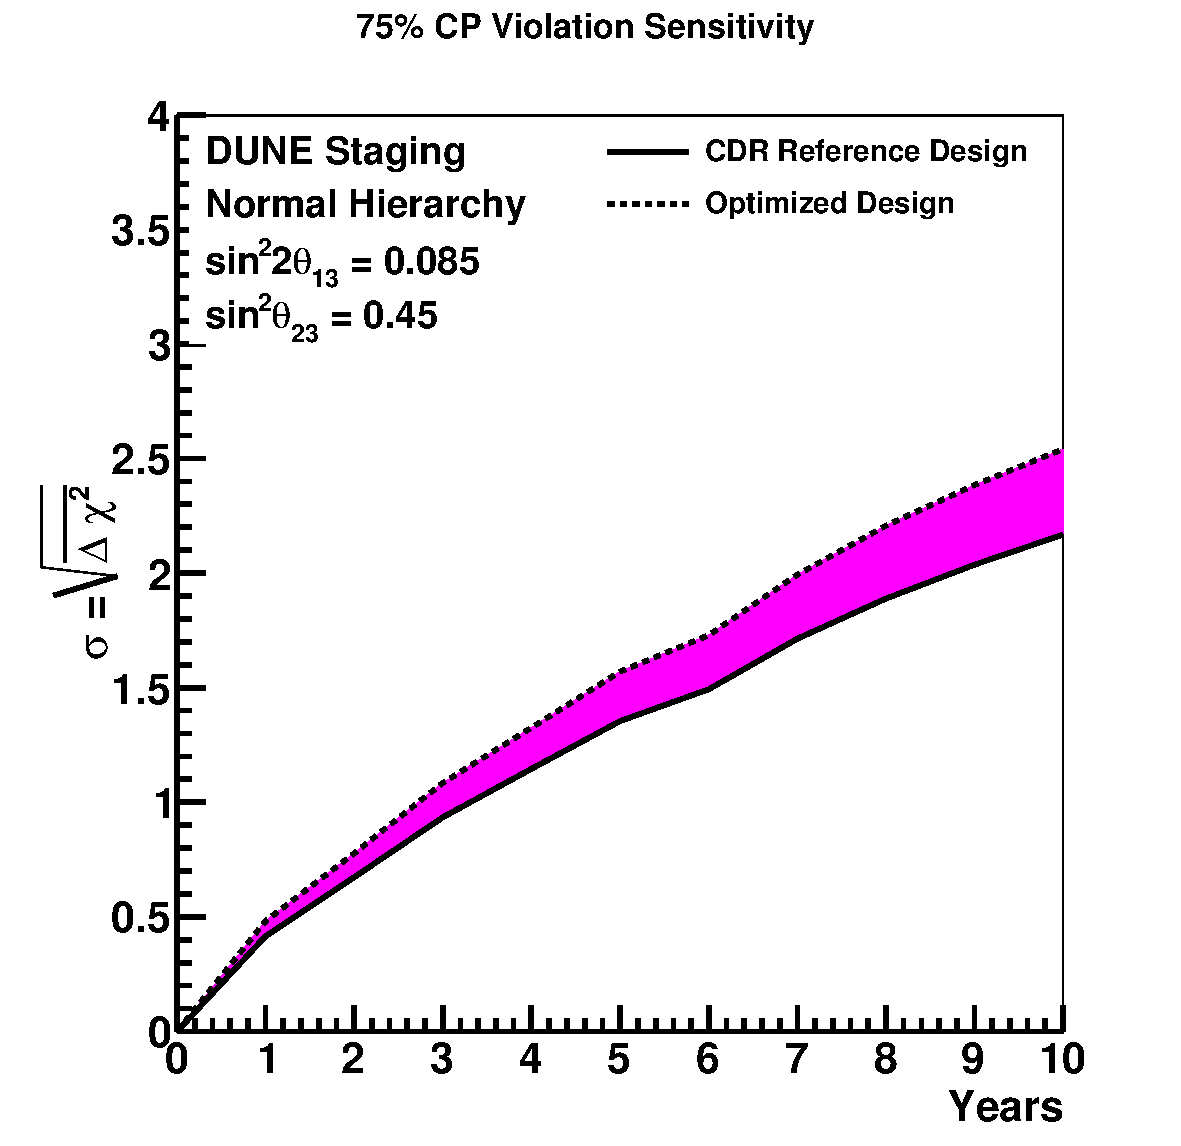
\includegraphics[width=0.49\textwidth]{cpv75_exp_staging.pdf}
\end{cdrfigure}

\section{Precision Oscillation Parameter Measurements}

% The value of \sinstt{23} is measured to be $>$~0.95 at 90\% CL 
% using atmospheric neutrino oscillations~\cite{Abe:2011ph}. 
The most precise measurement of $\sin^2\theta_{23}$ to date comes from T2K, $\sin^2\theta_{23}~=~0.514^{+0.055}_{-0.056}$~(normal hierarchy) and $\sin^2\theta_{23}~=~0.511~\pm~0.055$~(inverted hierarchy)~\cite{Abe:2015awa}.
This corresponds to a value of 
$\theta_{23}$ near 45\mbox{$^{\circ}$}, but leaves an ambiguity
as to whether the value of $\theta_{23}$ is in the lower octant 
(less than 45\mbox{$^{\circ}$}), the upper octant (greater than 45\mbox{$^{\circ}$}),
or exactly 45\mbox{$^{\circ}$}. 
The value of $\sin^2 \theta_{23}$ from
the global fit reported by~\cite{Gonzalez-Garcia:2014bfa} is $\sin ^2 \theta_{23} = 0.452
^{+0.052} _{-0.028} (1 \sigma)$ for normal hierarchy (NH), but the distribution of the $\chi^2$ from
the global fit has another local minimum --- particularly if the MH 
is inverted --- at $\sin^2 \theta_{23} = 0.579 ^{+0.025} _{-0.037} (1 \sigma)$. A
\emph{maximal} mixing value of $\sin^2 \theta_{23} =0.5$ is therefore still allowed
by the data and the octant is still largely undetermined.
A value of $\theta_{23}$ exactly equal to 45\mbox{$^{\circ}$} would indicate that 
$\nu_{\mu}$ and $\nu_{\tau}$ have equal contributions from $\nu_3$,
which could be evidence for a previously unknown symmetry. 
It is
therefore important experimentally to determine the value of
$\sin ^2 \theta_{23}$ 
with sufficient precision to determine 
the octant of $\theta_{23}$. 
The measurement of $\nu_\mu \rightarrow \nu_\mu$ oscillations is
sensitive to $\sin ^2 2 \theta_{23}$, whereas the measurement of
$\nu_\mu \rightarrow \nu_e$ oscillations is sensitive to $\sin^2
\theta_{23}$. 
A combination of both $\nu_e$ appearance and $\nu_\mu$ disappearance
measurements can probe both maximal mixing and the $\theta_{23}$
octant.  The $\Delta\chi^2$ metric is defined as:
\begin{eqnarray}
\Delta\chi^2_{octant} & = & |\chi^2_{\theta_{23}^{test}>45^\circ} - \chi^2_{\theta_{23}^{test}<45^\circ}|, \\ \nonumber
\end{eqnarray}
where the value of $\theta_{23}$ in the \emph{wrong} octant is constrained 
only to have a value within the \emph{wrong} octant (i.e., it is not required
to have the same value of $\sin^22\theta_{23}$ as the true value).
Figure~\ref{fig:octant} shows the sensitivity to determining the octant as a function of $\theta_{23}$.  Figure~\ref{fig:res_th23} shows the resolution of $\sin^2\theta_{23}$ as a function of exposure, assuming the true value is $\sin^2\theta_{23} = 0.45$ from the current global fit.

\begin{cdrfigure}[Octant sensitivity]{octant}{The significance with which DUNE can resolve the $\theta_{23}$ octant as a function of the true value of $\theta_{23}$. The green shaded band around the curve represents the range in sensitivity due to potential variations in the beam design and in the true value of \deltacp. The yellow shaded regions indicate the current 1-$\sigma$ and 3-$\sigma$ bounds on the value of $\theta_{23}$ from a global fit.  We assume an exposure that gives a 3-$\sigma$ measurement of CP violation for 75\% of the values of \deltacp.  See Figure~\ref{fig:cpv_exposure} for the possible range of exposure to acheive this significance.}
 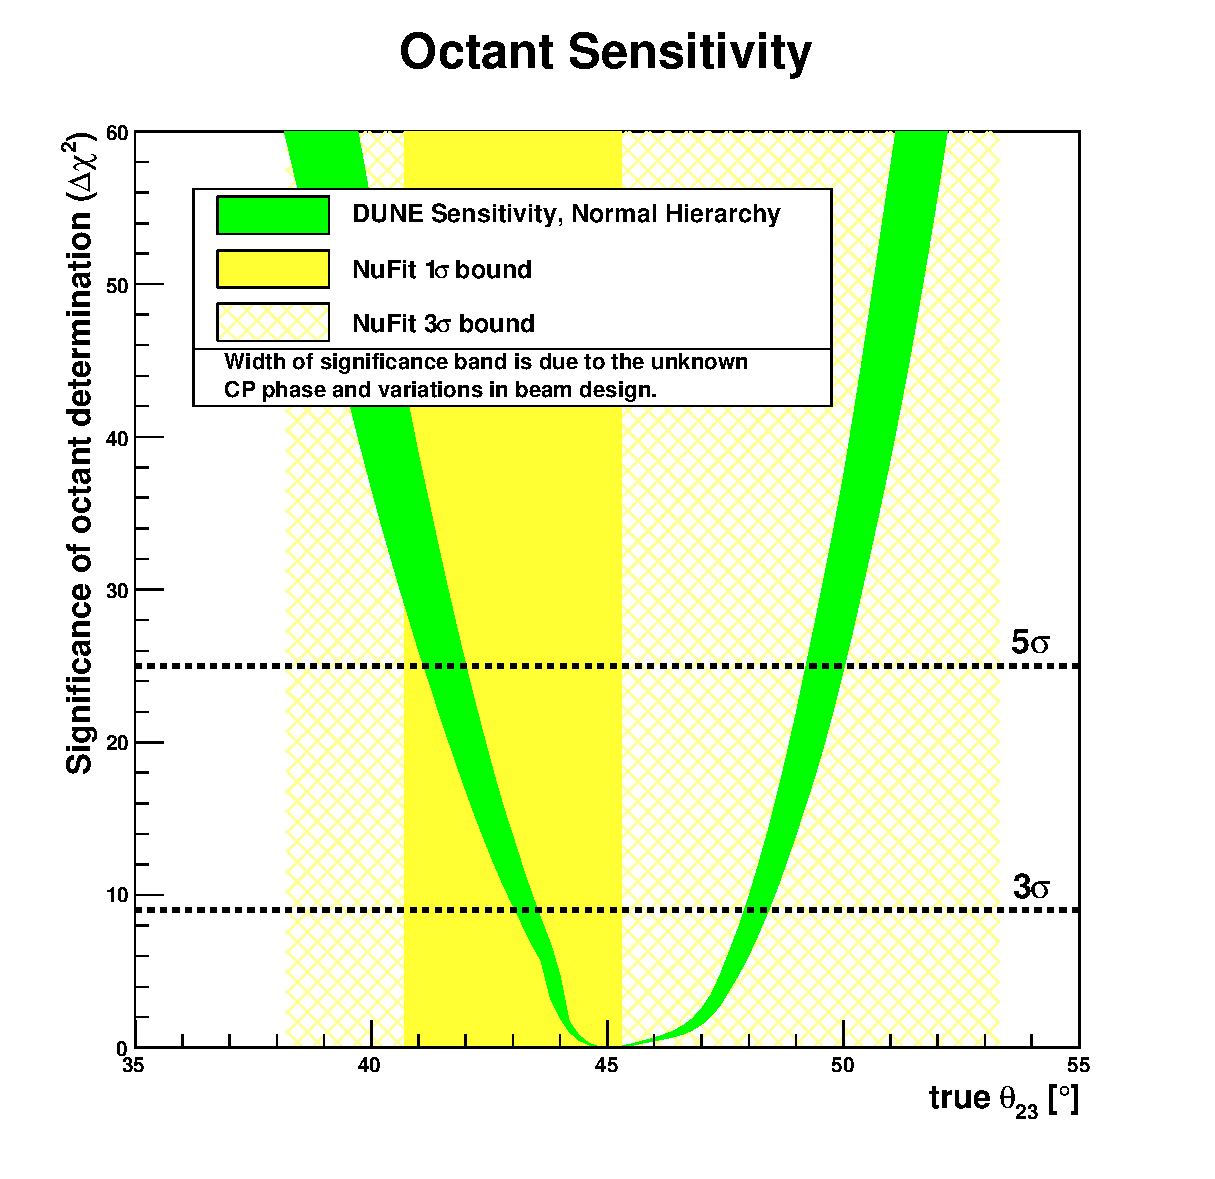
\includegraphics[width=0.7\textwidth]{octant_chi2_exp890}
\end{cdrfigure}

\begin{cdrfigure}[Resolution of $\sin^2\theta_{23}$ as a function of exposure]{res_th23}{The resolution of a measurement of $\sin^2\theta_{23}$ as a function of exposure assuming normal MH and $\sin^2\theta_{23} = 0.45$ from the current global fit. The shaded region represents the range in sensitivity due to potential variations in the beam design.  }
 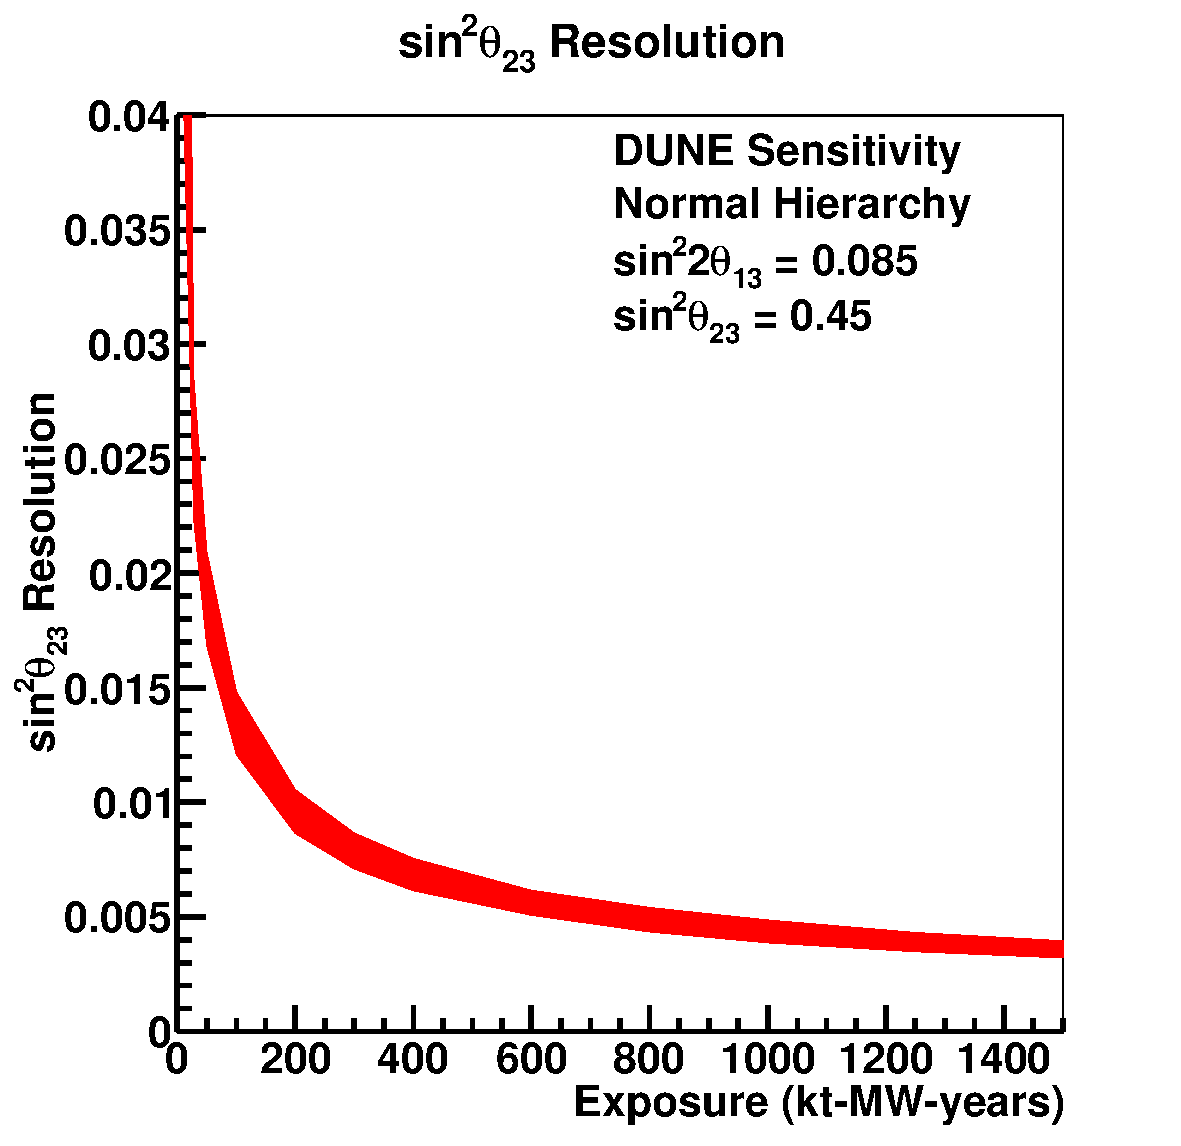
\includegraphics[width=0.7\textwidth]{res_th23_exp}
\end{cdrfigure}


As mentioned in Section~\ref{sec:physics-lbnosc-cpv}, DUNE will seek not only to demonstrate explicit CP violation by observing a difference in the neutrino and antineutrino oscillation probabilities, but also to measure the value of the parameter \deltacp.  Figure~\ref{fig:res_cp} shows the resolution of \deltacp as a function of exposure for a CP-conserving value (\deltacp = 0) and the value that gives the maximum CP violation for normal MH (\deltacp = 90\mbox{$^{\circ}$}).

\begin{cdrfigure}[Resolution of \deltacp as a function of exposure]{res_cp}{The resolution of a measurement of \deltacp as a function of exposure assuming normal MH.  The resolution is shown for a CP-conserving value (\deltacp = 0) and the value that gives the maximum CP violation for normal MH (\deltacp = 90\mbox{$^{\circ}$}). The shaded region represents the range in sensitivity due to potential variations in the beam design.  }
 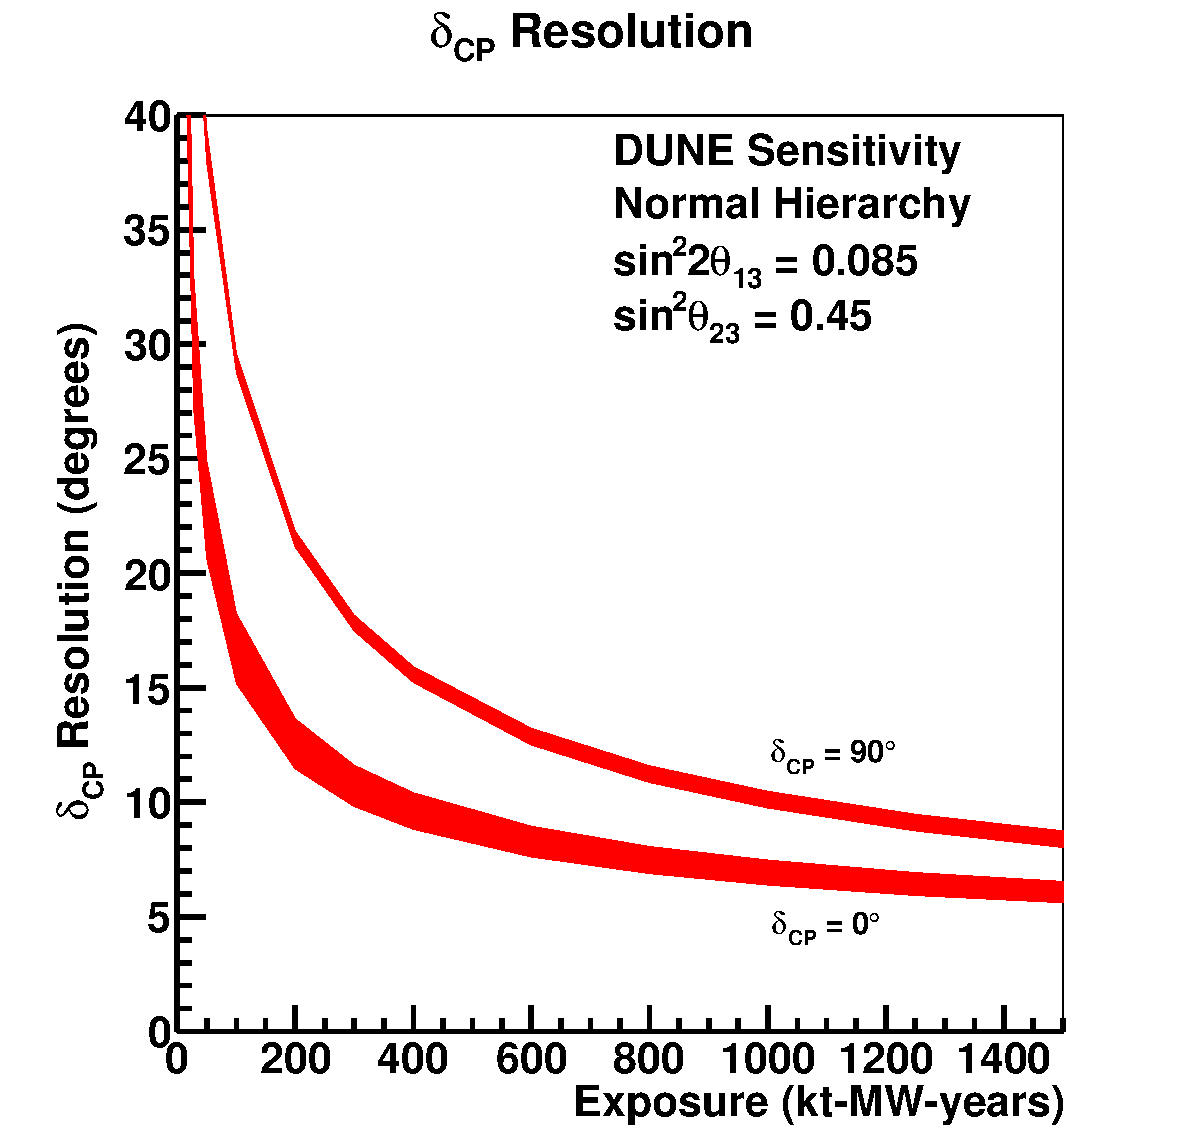
\includegraphics[width=0.7\textwidth]{res_dcp_exp}
\end{cdrfigure}

The rich oscillation structure that can be observed by DUNE and the
excellent particle identification capability of the detector
will enable precision measurement  in a single experiment of all the mixing parameters
governing $\nu_1$-$\nu_3$ and $\nu_2$-$\nu_3$ mixing. Theoretical models probing quark-lepton
universality predict specific values of the mixing angles and the
relations between them. The
mixing angle $\theta_{13}$ is
expected to be measured accurately in reactor experiments by the end
of the decade with a precision that will be limited by
systematics. 
The combined statistical and systematic uncertainty on the value of $\sin ^ 2 2
\theta_{13}$ from the Daya Bay reactor neutrino experiment, which has
the lowest systematics, is currently $\sim6$\% ($\sin^22\theta_{13} = 0.084\pm0.005$),
with a projected uncertainty of $\sim$3\% by 2017~\cite{Zhang:2015fya}.
While the constraint on $\theta_{13}$ from the reactor experiments will be
important in the
early stages of DUNE for determining CP violation, measuring
\deltacp and determining the $\theta_{23}$ octant, 
DUNE itself will eventually be able to measure
$\theta_{13}$ independently with a similar precision to that expected from the reactor experiments. 
Whereas the reactor experiments measure $\theta_{13}$ using $\overline{\nu}_e$
disappearance, DUNE will measure it through $\nu_e$ and
$\overline{\nu}_e$ appearance, thus providing an independent constraint on
the three-flavor mixing matrix.   Figure~\ref{fig:res_th13} shows the resolution of $\sin^22\theta_{13}$ as a function of exposure, assuming the true value is $\sin^22\theta_{13} = 0.085$ from the current global fit.

\begin{cdrfigure}[Resolution of $\sin^22\theta_{13}$ as a function of exposure]{res_th13}{The resolution of a measurement of $\sin^22\theta_{13}$ as a function of exposure assuming normal MH and $\sin^22\theta_{13} = 0.085$ from the current global fit. The shaded region represents the range in sensitivity due to potential variations in the beam design.  }
 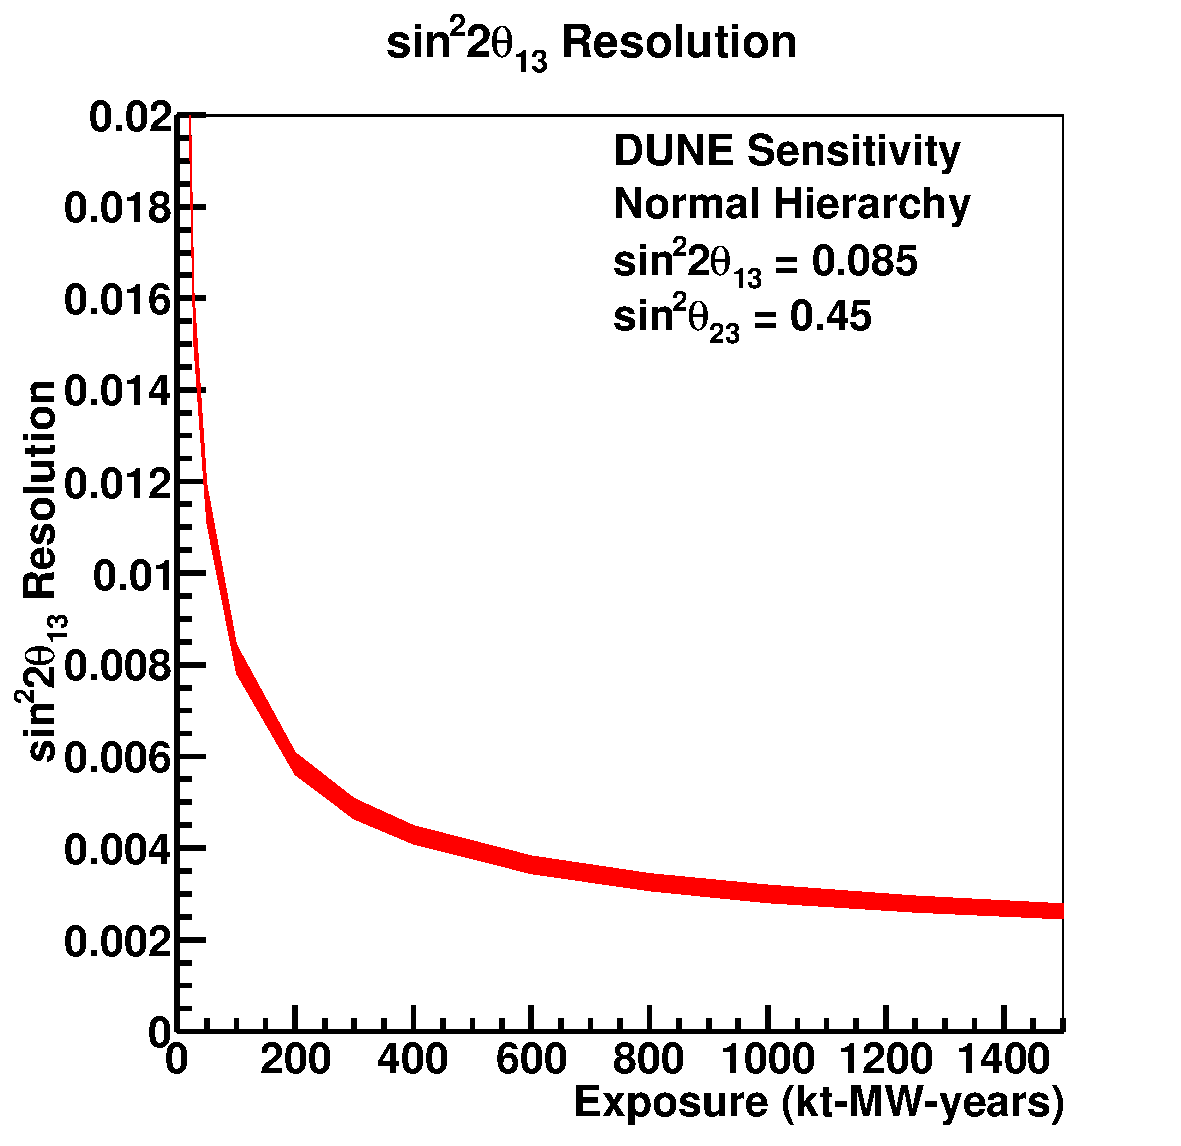
\includegraphics[width=0.7\textwidth]{res_th13_exp}
\end{cdrfigure}

DUNE can also significantly improve the
resolution on the larger mass splitting beyond the precision of current experiments.  The current best fit value for $\Delta m^2_{32}$ from MINOS is $|\Delta m^2_{32}| = (2.34\pm0.09)\times10^{-3}$~eV$^2$ (normal hierarchy) and $|\Delta m^2_{32}| = (2.37^{+0.11}_{-0.07})\times10^{-3}$~eV$^2$ (inverted hierarchy)~\cite{Sousa:2015bxa}, with comparable precision acheived by both Daya Bay and T2K. The
precision on $\Delta m^2_{31}$ will ultimately depend on tight control
of energy-scale systematics.  Figure~\ref{fig:res_dm2} shows the expected resolution of \dm{31} as a function of exposure, assuming the true value is \dm{31} = $2.457\times10^{-3}$~eV$^2$ from the current global fit.

\begin{cdrfigure}[Resolution of \dm{31} as a function of exposure]{res_dm2}{The resolution of a measurement of \dm{31} as a function of exposure assuming the true value is \dm{31} = $2.457\times10^{-3}$~eV$^2$ from the current global fit. The shaded region represents the range in sensitivity due to potential variations in the beam design.  }
 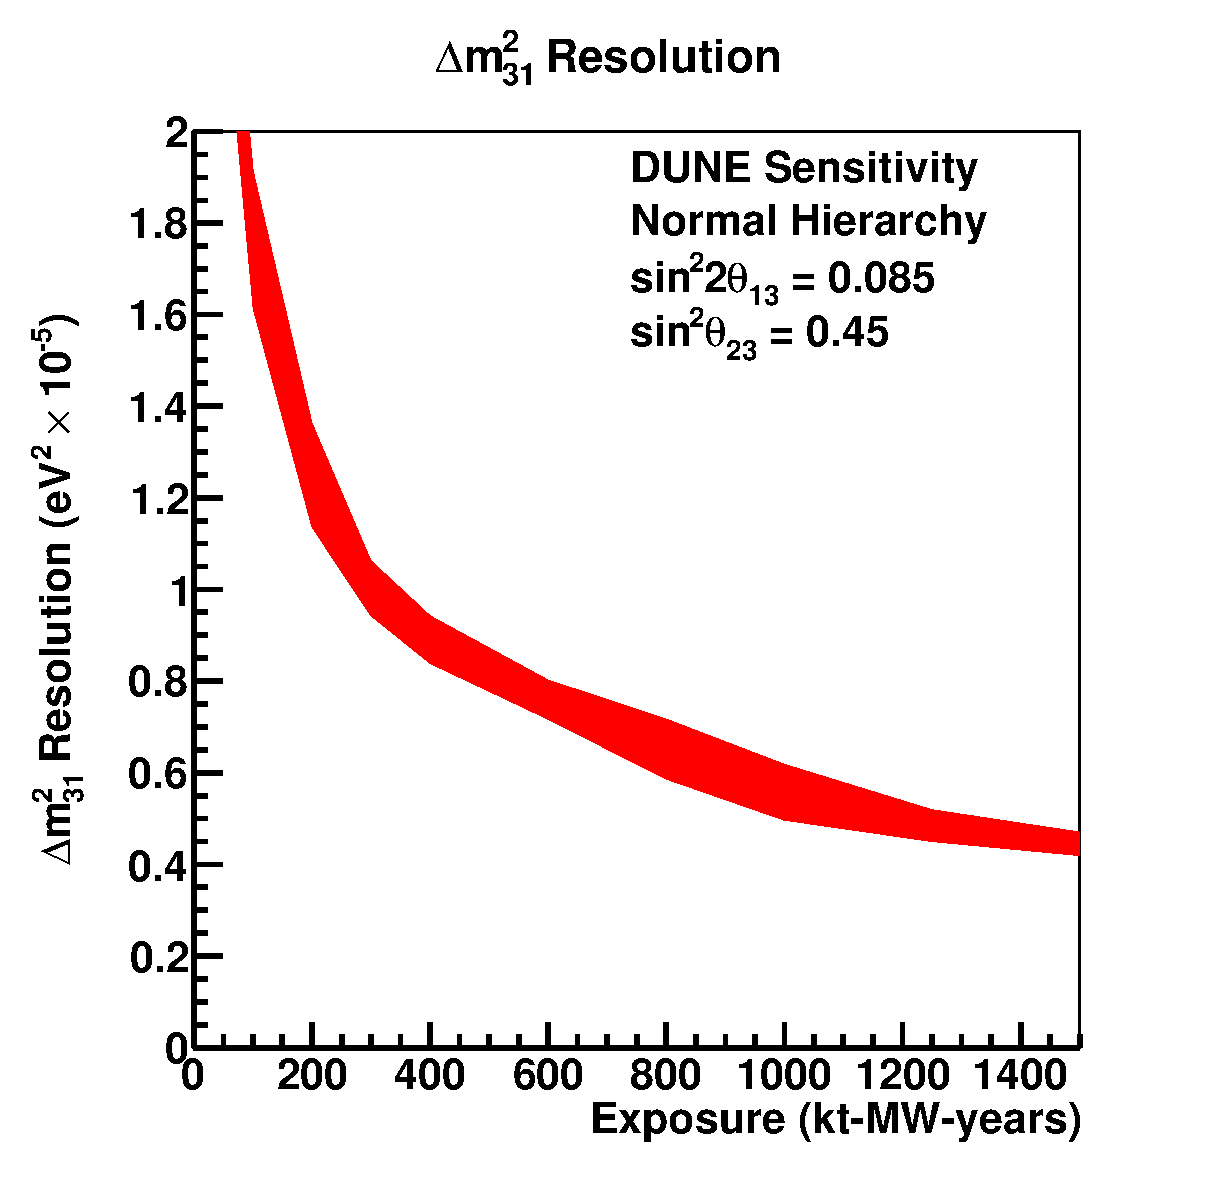
\includegraphics[width=0.7\textwidth]{res_dm_exp}
\end{cdrfigure}

\section{Testing the 3-flavor Paradigm and the Standard Model}
\label{sec:physics-lbnosc-3nutests}

Due to the very small masses and large mixing of neutrinos, their oscillations over a long distance
  act as an exquisitely precise interferometer with high sensitivity to very small perturbations caused by 
  new physics phenomena, such as:
  \begin{itemize}
  \item nonstandard interactions in matter that manifest in
    long-baseline oscillations as deviations from the three-flavor mixing model
  \item new long-distance potentials arising from discrete symmetries
    that manifest as small perturbations on neutrino and antineutrino
    oscillations over a long baseline
  \item sterile neutrino states that mix with the three known active neutrino states
  \item large compactified extra dimensions from String Theory models that manifest through mixing
    between the Kaluza-Klein states and the three active neutrino
    states
   \item Lorentz and CPT violation due to an underlying Planck-scale theory that manifest through sidereal dependence on the neutrino oscillation probability
  \end{itemize}
  Full exploitation of DUNE's sensitivity to such new phenomena
  will require high-precision predictions of the unoscillated
  neutrino flux at the far detector and large exposures. Studies will be conducted to understand the
limits that DUNE could impose relative to current limits and those expected from other experiments.
  
\subsection{Search for Nonstandard Interactions}

For $\nu_{\mu,e} \rightarrow \nu_{e,\mu}$ 
oscillations that occur as the neutrinos propagate through matter,  
the coherent forward scattering of $\nu_e$'s on electrons in matter 
modifies the energy and path-length dependence of the vacuum oscillation 
probability in a way that depends on the magnitude \emph{and} sign of $\Delta m^2_{31}$. 
This is  the Mikheyev-Smirnov-Wolfenstein (MSW) effect~\cite{Mikheev:1986gs,Wolfenstein:1977ue}.
NC nonstandard interactions (NSI) may be interpreted as nonstandard
matter effects that are visible only in a far detector at a
sufficiently long baseline. 
They can be parameterized as new contributions
to the MSW matrix in the neutrino-propagation Hamiltonian~\cite{Valle:1987gv,Roulet:1991sm}:

\begin{equation}
  H = U \left( \begin{array}{ccc}
           0 &                    & \\
             & \Delta m_{21}^2/2E & \\
             &                    & \Delta m_{31}^2/2E
         \end{array} \right) U^\dag + \tilde{V}_{\rm MSW} \,,
\end{equation}
with
\begin{equation}
  \tilde{V}_{\rm MSW} = \sqrt{2} G_F N_e
\left(
  \begin{array}{ccc}
    1 + \epsilon^m_{ee}       & \epsilon^m_{e\mu}       & \epsilon^m_{e\tau}  \\
        \epsilon^{m*}_{e\mu}  & \epsilon^m_{\mu\mu}     & \epsilon^m_{\mu\tau} \\
        \epsilon^{m*}_{e\tau} & \epsilon^{m*}_{\mu\tau} & \epsilon^m_{\tau\tau}
  \end{array} 
\right)
\end{equation}

Here, $U$ is the leptonic mixing matrix, and the $\epsilon$-parameters give the
magnitude of the NSI relative to standard weak interactions.  For new physics
scales of a few hundred GeV,  a value of $|\epsilon| \leq 0.01$ is
expected~\cite{Davidson:2003ha,GonzalezGarcia:2007ib,Biggio:2009nt,Barranco:2007ej,Escrihuela:2011cf}.
DUNE's 1300-km baseline provides an advantage in the detection of NSI relative
to existing beam-based experiments with shorter baselines.
Only atmospheric-neutrino experiments have longer baselines, but the sensitivity
of these experiments to NSI is limited by systematic effects. See \cite{Adams:2013qkq}
for potential sensitivities to these parameters at a 1300-km baseline.

\subsection{Search for Long-Range Interactions}

The small scale of neutrino-mass differences implies that minute
differences in the interactions of neutrinos and antineutrinos with
currently unknown particles or forces may be detected through 
perturbations to the time evolution of the flavor eigenstates.  
The longer the experimental
baseline, the higher the sensitivity to a new long-distance potential
acting on neutrinos. For example, some of the models for such
long-range interactions (LRI) as described in~\cite{Davoudiasl:2011sz} could contain discrete symmetries that
stabilize the proton and give rise to a dark-matter candidate particle,
thus providing new
connections between neutrino, proton decay and dark matter
experiments. The longer baseline of DUNE improves the sensitivity to
LRI beyond that possible with the current generation of long-baseline
neutrino experiments. The sensitivity will be determined by the amount
of $\nu_\mu/\overline{\nu}_\mu$-CC statistics accumulated and the accuracy
with which the unoscillated and oscillated $\nu_\mu$ spectra can be
determined.

\subsection{Search for Mixing between Active and Sterile Neutrinos}

Several recent anomalous experimental results count among their possible
interpretations phenomena that do not fit in the three-flavor mixing
model~\cite{Aguilar:2001ty,AguilarArevalo:2007it,Aguilar-Arevalo:2013pmq,Mention:2011rk,Giunti:2010zu}, 
and searches for evidence of one or more sterile neutrino states are ongoing.
At DUNE, searches for active-sterile neutrino mixing can be
conducted by examining the NC event rate at the far detector and
comparing it to a precise estimate of the expected rate extrapolated
from $\nu_\mu$ flux measurements from the  
near detector and from 
beam and detector simulations. Observed deficits in the NC rate could be evidence for mixing between the
active neutrino states and unknown sterile neutrino states. The most recent such search
in a long-baseline experiment was conducted by the MINOS
experiment~\cite{Adamson:2011ku,Sousa:2015bxa}.  DUNE will provide a unique
opportunity to revisit this search over a large
range of neutrino energies and a longer baseline. The large detector mass and high beam power will
allow a high-statistics sample of NC interactions to be collected.
The high-resolution LArTPC far detector
will enable a coarse measurement of the incoming neutrino
energy in a NC interaction by using the event topology and correcting
for the missing energy of the invisible neutrino.  Both the
energy spectrum and the rate of NC interactions will be measured
with high precision at both near and far detectors.

\subsection{Search for Large Extra Dimensions}

Several theoretical models propose that right-handed neutrinos
propagate in large compactified extra dimensions, whereas the standard
left-handed neutrinos are confined to the four-dimensional 
brane~\cite{Machado:2011wx}. Mixing between the right-handed \emph{Kaluza-Klein} 
modes and the standard
neutrinos would change the mixing patterns predicted by
the three-flavor model. The effects could manifest, for example, as distortions in the
disappearance spectrum of $\nu_\mu$.  The rich oscillation
structure visible in DUNE, measured with
its high-resolution detector
using both beam and atmospheric oscillations,
could provide further opportunities to probe for
this type of new physics.

\subsection{Search for Lorentz and CPT Violation}

Lorentz invariance and its associated CPT symmetry
are foundational aspects of the Standard Model. However, the Standard Model is thought to be a low-energy limit of a more fundamental theory that unifies quantum physics with gravity at the Planck
scale. As a result, an underlying theory can induce violations of Lorentz invariance and
violations of CPT symmetry that can generate experimentally observable signals of Planck-scale physics.
The Standard-Model Extension (SME)~\cite{Colladay:1996iz,Colladay:1998fq,Kostelecky:2003fs} is an effective field theory that contains the Standard Model, general relativity, and all possible operators that break Lorentz symmetry. (Since CPT violation implies Lorentz violation, the SME necessarily includes operators that break CPT symmetry.)  Within the SME framework, the probability for neutrino oscillations depends on the direction of neutrino propagation within a Sun-centered inertial frame~\cite{Kostelecky:2003cr,Kostelecky:2011gq}.  For a long-baseline experiment with both the neutrino beam source and detector fixed to the surface of the Earth, the Earth's rotation causes the direction of neutrino propagation to change with sidereal time.  The SME theory thus predicts a sidereal dependence of the observed beam neutrino rate.  DUNE has the potential to perform studies that explore regimes never previously investigated and to improve existing
sensitivities obtained in other neutrino experiments.
For example, the baseline of 1300~km offers an advantage because the sensitivity to 
% the coefficients for
Lorentz and CPT violation grows linearly with the baseline.   The
beam orientation for DUNE is different from other experiments such as MINOS or T2K, so
the combinations of coefficients for Lorentz and CPT violation appearing in the DUNE mixing probabilities are
distinct. Additionally, the wide range of energy for the beam neutrinos and the ability to investigate both neutrino and antineutrino channels are advantageous.

\section{Neutrino Beam Requirements}
\label{sec:physics-lbnosc-beam-req}
The LBNF neutrino facility at Fermilab utilizes a conventional
horn-focused neutrino beam produced from pion and kaon decay-in-flight. It will
aim the neutrino beam toward the 
the DUNE far detector located 1,300 km away at the Sanford Underground
Research Facility. LBNF must be designed for approximately twenty years of operation, in order to provide adequate exposure for the DUNE experiment. During its lifetime, the facility must be able to accommodate various target and focusing configurations to enable tunability 
in the neutrino energy spectrum, and must be suitable for upgraded targets and horns as technology improves and the primary proton beam power increases. Such
flexibility is an essential requirement for a facility that will operate over multiple decades. The energy range of the neutrino beam must be adaptable, in order to address new questions in neutrino physics that may come up during such a long period.

The DUNE experiment requires that the LBNF facility
\begin{enumerate} 
\item Shall generate a high intensity, wide-band neutrino beam,
  selectable for muon neutrinos or muon antineutrinos with a low
  contamination of electron and wrong-sign neutrinos.
\item Shall fully cover the energy range of the first oscillation
  node, which ranges from $\sim1$ GeV to $\sim5$ GeV and peaks at
  $\sim2.4$ GeV for a 1300 km baseline. It shall also provide a
  neutrino flux as high as reasonably achievable around the second
  oscillation node, which peaks at $\sim0.8$ GeV, possibly requiring
  a dedicated focusing configuration. An energy range extending
  from 0.5 to 5 GeV is necessary to provide the maximum sensitivity
  for CP violation searches and the determination of the neutrino mass
  hierarchy. Focusing configurations providing neutrino energies
  higher than 5 GeV may also be required for a full exploration of the
  three-neutrino paradigm and to address anomalies that may arise
  during the two decade lifetime of the experiment. 
\item Shall be capable of operating with a single-turn extracted primary proton beam
  from the Main Injector with greater than 2 MW of power. It must be
  able to accept proton momenta between 60 and 120 GeV/c, since this
  will enable some optimization of the neutrino energy spectrum. The
  capability to lower the energy of the protons is also an
  effective way to reduce the wrong-sign component in the neutrino
  flux. A reduction of up to $\sim15 \%$ in beam power is expected as
  the momentum of the primary protons decreases from 120 to 60 GeV/c,
  since the Main Injector cycle time does not scale linearly with the
  energy of the accelerated protons.  Table~\ref{tab:beam_req_pot} gives a
  summary of the expected number of protons on target per year at
  various momenta assuming a combined uptime and efficiency of 56\%. 
\item Shall be built to provide a realistic estimation and whenever
  possible a reduction of the systematic errors on the neutrino flux prediction, e. g. by adequate requirements on the alignment tolerances of the beamline components. Dedicated hadroproduction measurements from 60-120 GeV/c protons will be needed to reduce the uncertainty on the neutrino flux components, both from pion and kaon decays. 
\item Shall be built to ensure the stability of the produced neutrino flux by minimizing variations in targeting angle and position of the primary proton beam, short and long term displacement of the components of the focusing system, and variations in the current pulse to the horns.
\end{enumerate}
\begin{cdrtable}[Expected POT per year at various primary proton beam
  momenta.]{ccc}{beam_req_pot}{Expected POT per year at various
    primary proton beam momenta.}
Proton Momentum (GeV/c) & Expected Beam Power (MW) & Expected POT/year
\\
\toprowrule 
120 & 1.2 & 1.1e21 \\
80 & 1.07 & 1.47e21 \\
60 & 1.03 & 1.89e21 \\
\end{cdrtable}

\subsection{Reference Beam Design}
\label{sec:reference-design-focusing-system}
The reference beam design is described in detail in Volume 3. It
includes a target similar to the one used for the low-energy tune of
the NuMI beam~\cite{numitdr}, but with a larger thickness to
accommodate the 1.2 MW primary proton beam, and focusing horns
essentially identical to those currently in operation in the NuMI
beamline~\cite{numitdr}. The target consists of 47 graphite segments,
for a total length of 95 cm including the space between segments,
corresponding to two interaction lengths. The upstream face of the
first segment is positioned 45 cm upstream of the first focusing horn to ensure sufficient clearance of the target's downstream end from the horn inner conductor. The separation of the upstream faces of the two horns has been decreased to 6.6 m, compared to the 10 m distance for the low-energy tune of the NuMI beam, to slightly enhance the neutrino flux at lower energies. A helium-filled decay pipe, 4 m in diameter and 204 m in length, provides the decay volume for the secondary pions to decay to muon neutrinos. 

Neutrino fluxes for the reference beam are shown in
Figure~\ref{fig:beam_req_reference_flux} for a 120 GeV primary proton
beam.  Lowering the momentum of the primary proton beam increases
right-sign neutrino flux at low energies and decreases wrong-sign
contamination.  Figure~\ref{fig:beam_req_proton_energy} shows current
projections of power versus proton energy, we estimate that 
$\delta_{CP}$ and mass hierarchy sensitivities improve modestly as
proton energy decreases, until approximately 60 GeV, below which the
Main Injector cycle time becomes constant with proton energy, causing
beam power to drop sharply.   Unless otherwise noted, results
throughout this volume assume an 80 GeV proton beam, corresponding to
the optimal momentum whose technical feasibility has been thoroughly
studied.  

Another handle for tuning the neutrino energy
spectrum of the reference beam is modification of the distance between
the target and the first focusing horn.  The expected fluxes for three
different configurations are shown in
Figure~\ref{fig:beam_req_lemehe}. The improvement in flux for each configuration with a longer decay pipe length of 250 m is also shown.

\begin{cdrfigure}[Neutrino fluxes for the reference focusing 
  system.]{beam_req_reference_flux}{Neutrino fluxes for the reference 
    focusing system operating in neutrino mode (left) and antineutrino 
    mode (right), generated with a 120 GeV/c primary proton beam.} 
\centering 
\begin{minipage}{0.45\textwidth}
\centering 
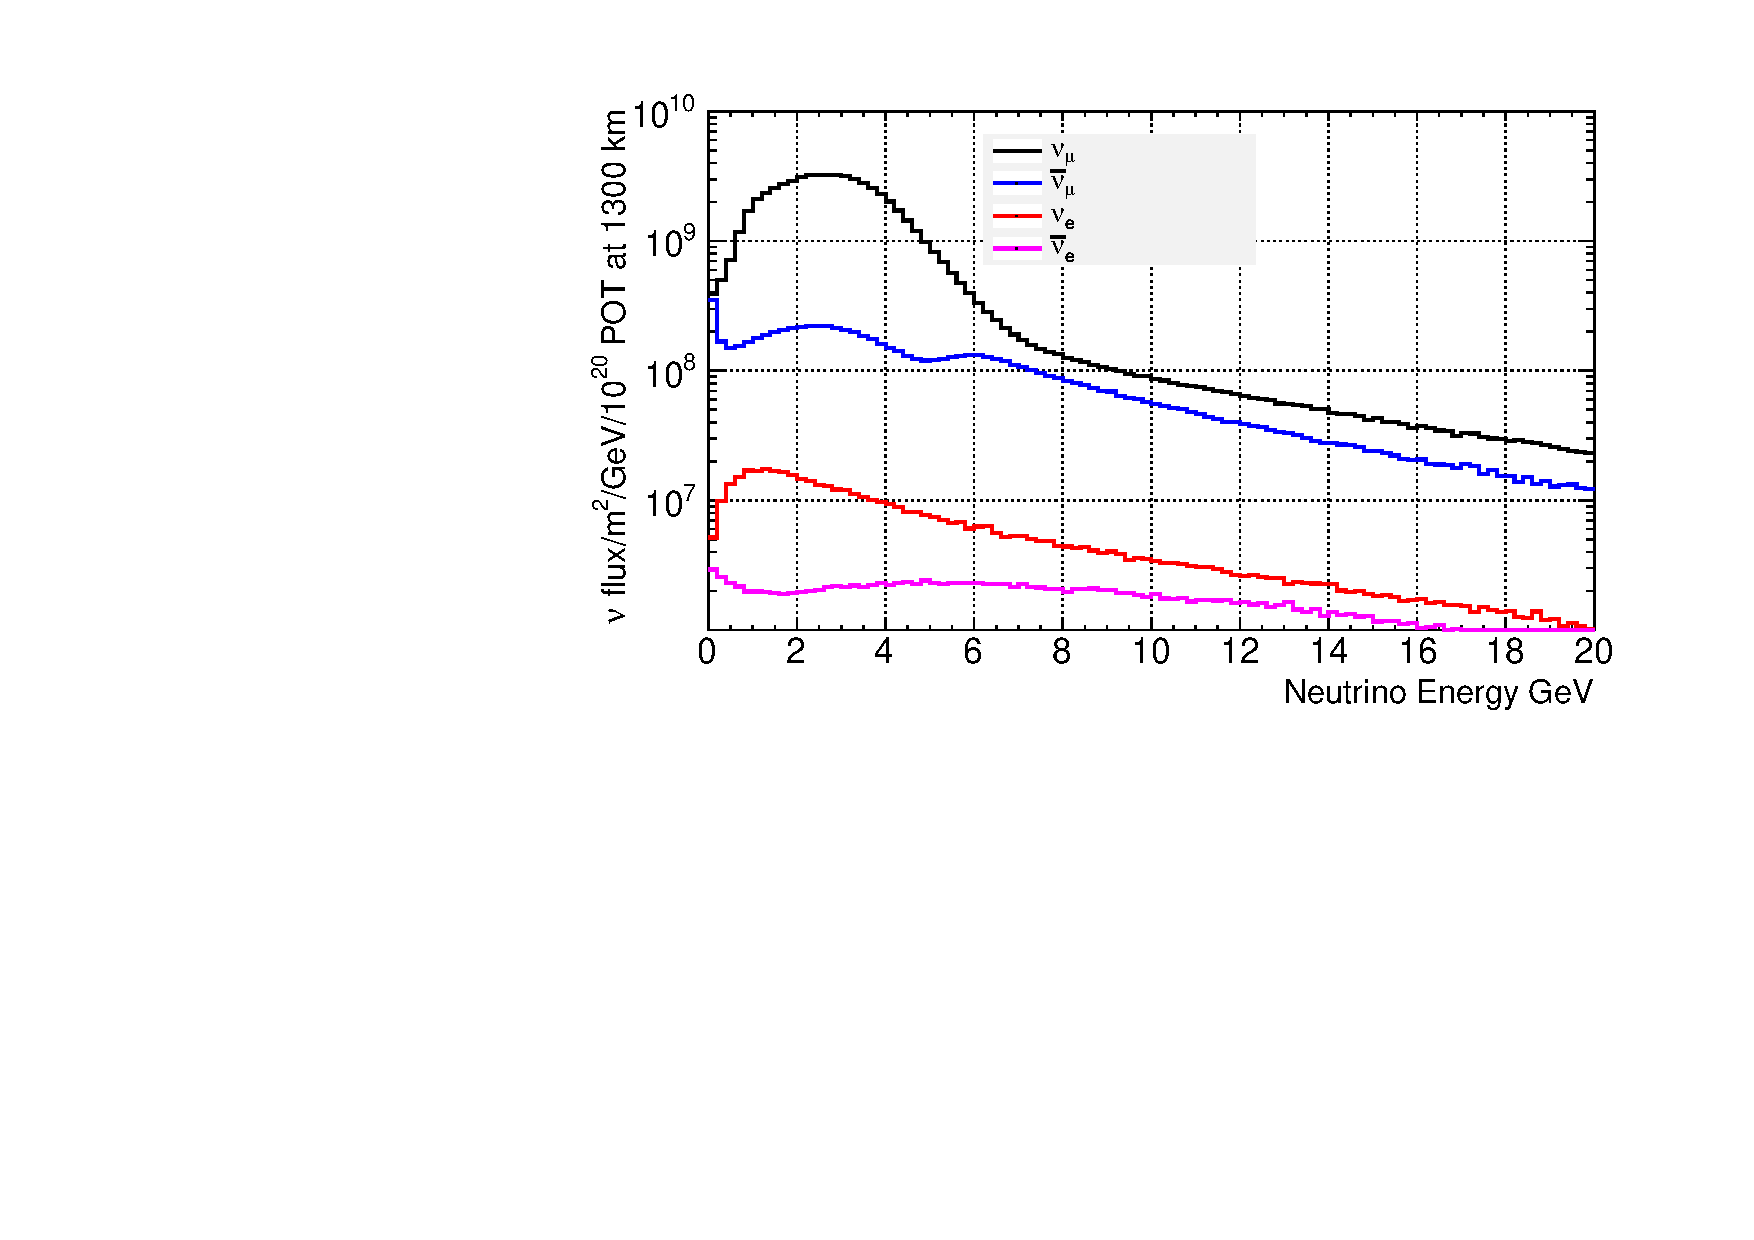
\includegraphics[width=1.0\textwidth]{flux_FHC}
\end{minipage}\hfill 
\begin{minipage}{0.45\textwidth}
\centering 
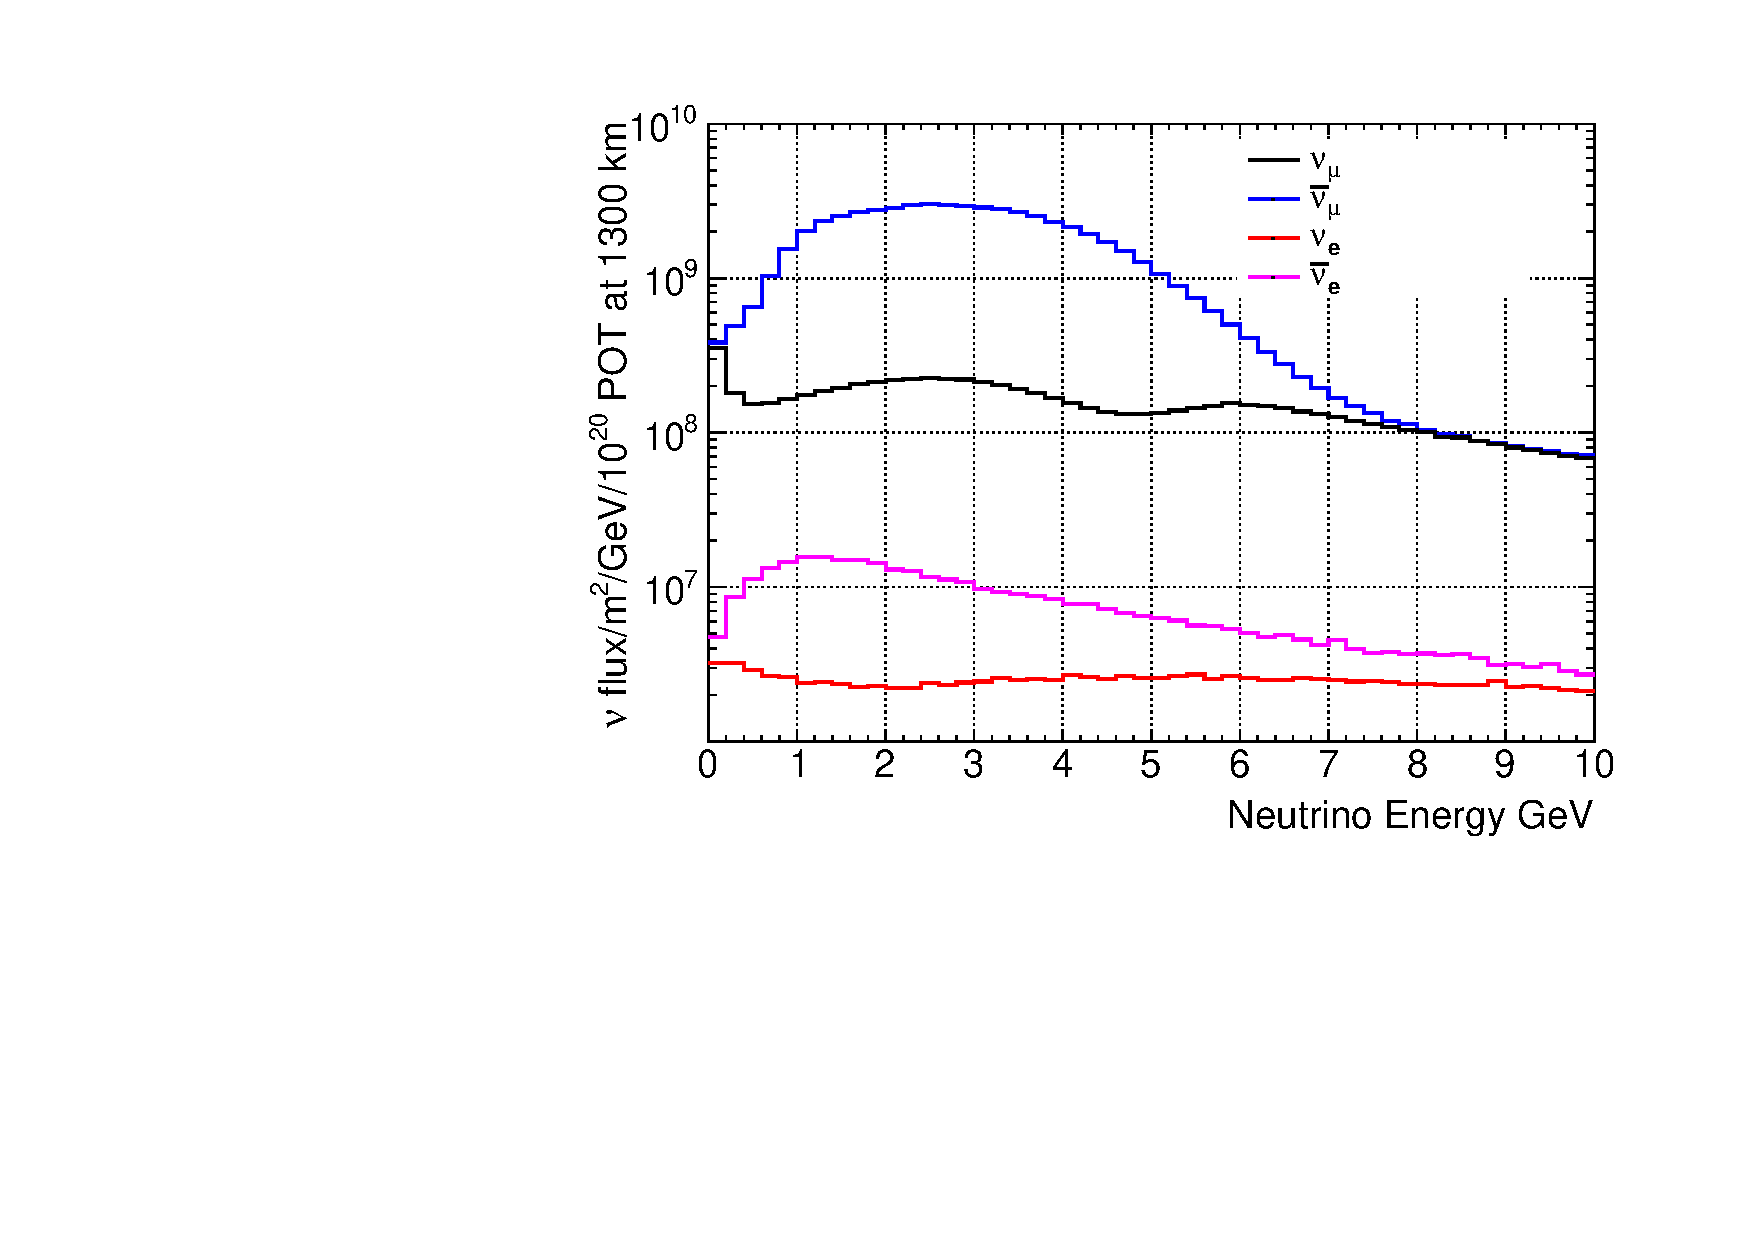
\includegraphics[width=1.0\textwidth]{flux_RHC}
\end{minipage}
\end{cdrfigure}

\begin{cdrfigure}[CP and mass hierarchy sensitivity versus proton 
  momentum.]{beam_req_proton_energy}{Minimum mass hierarchy
    sensitivity (left) and 
    coverage of 75\% of possible values of $\delta_{CP}$ (right) as a
    function of proton momentum.  {\it Produced using the Fast MC.
      Will be updated to use latest sensitivity infrastructure and to
      display a band ranging from reference to optimized beam.}}
\centering 
\begin{minipage}{0.45\textwidth}
\centering 
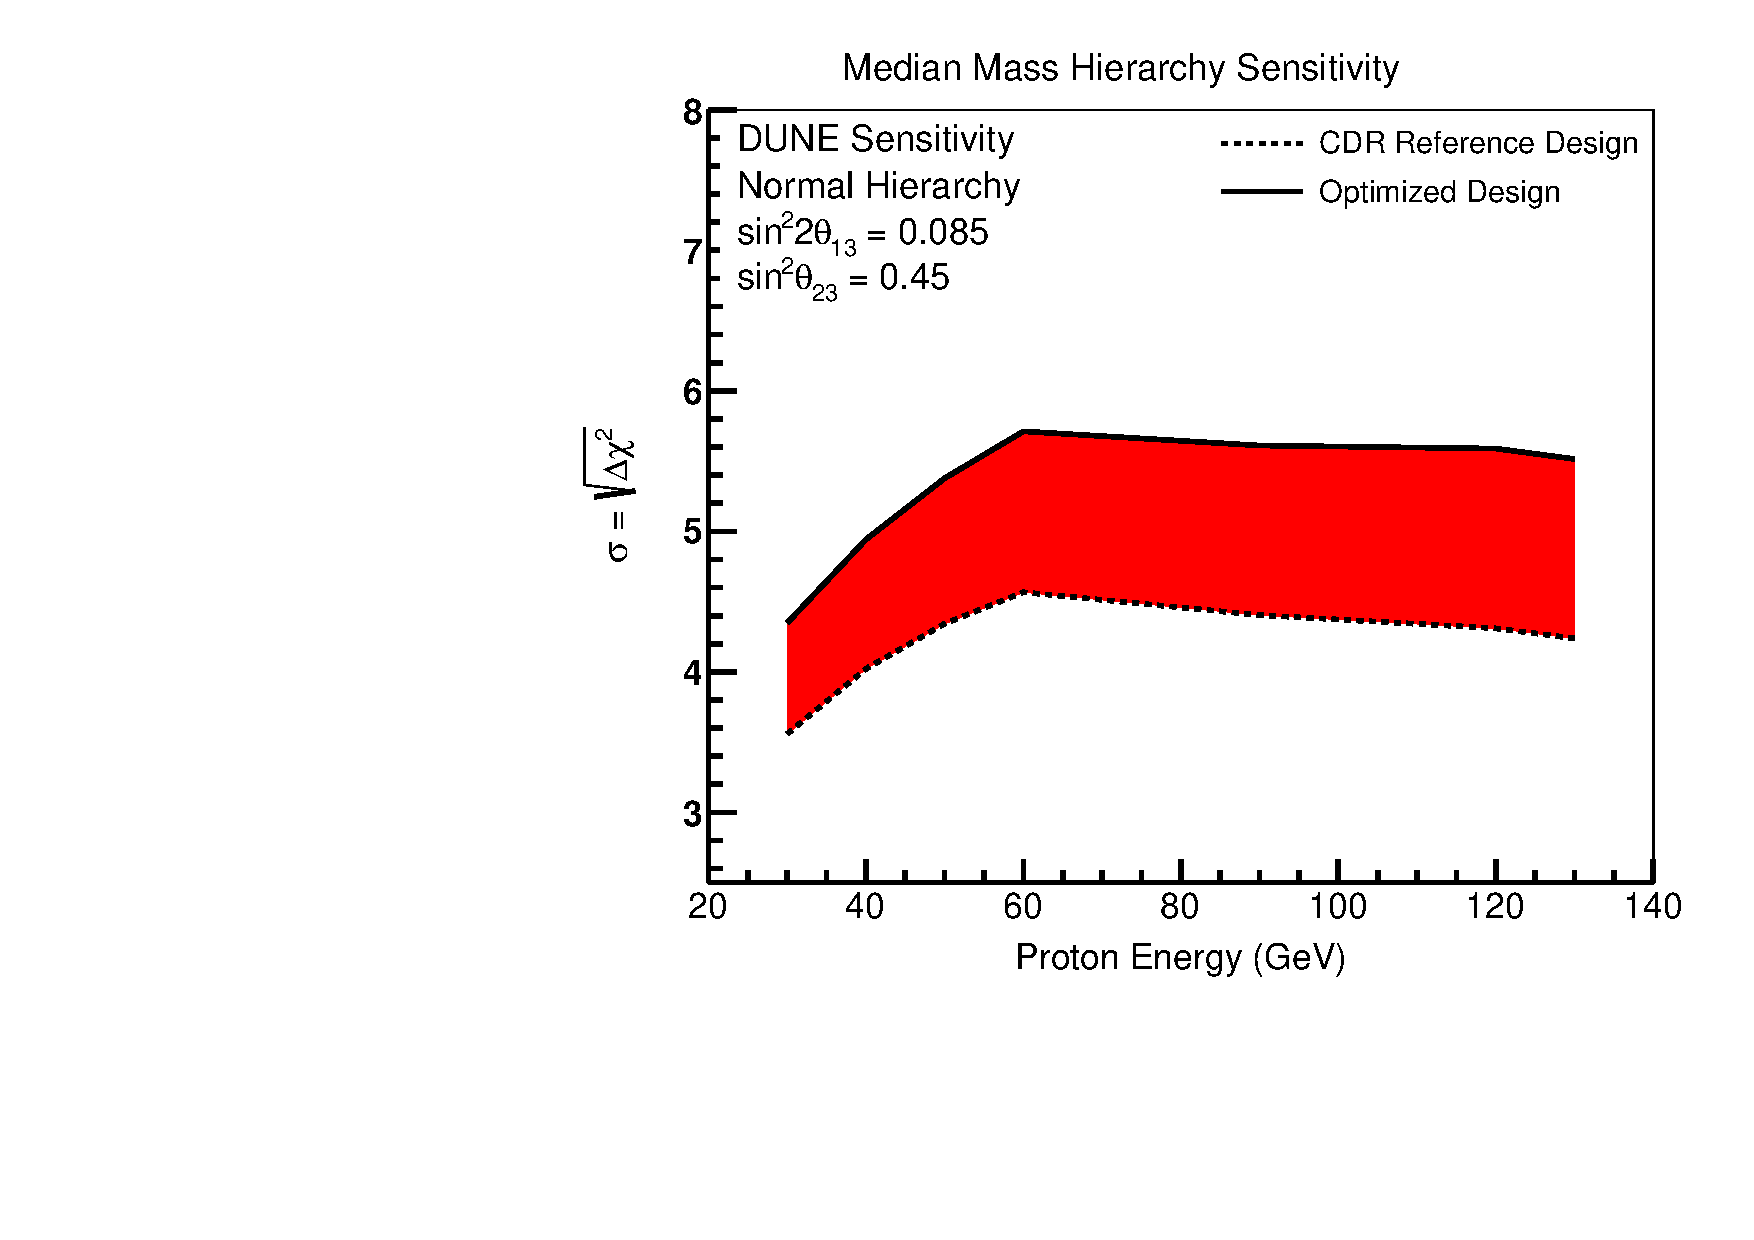
\includegraphics[width=1.0\textwidth]{summary_rp_nh_mh}
\end{minipage}\hfill 
\begin{minipage}{0.45\textwidth}
\centering 
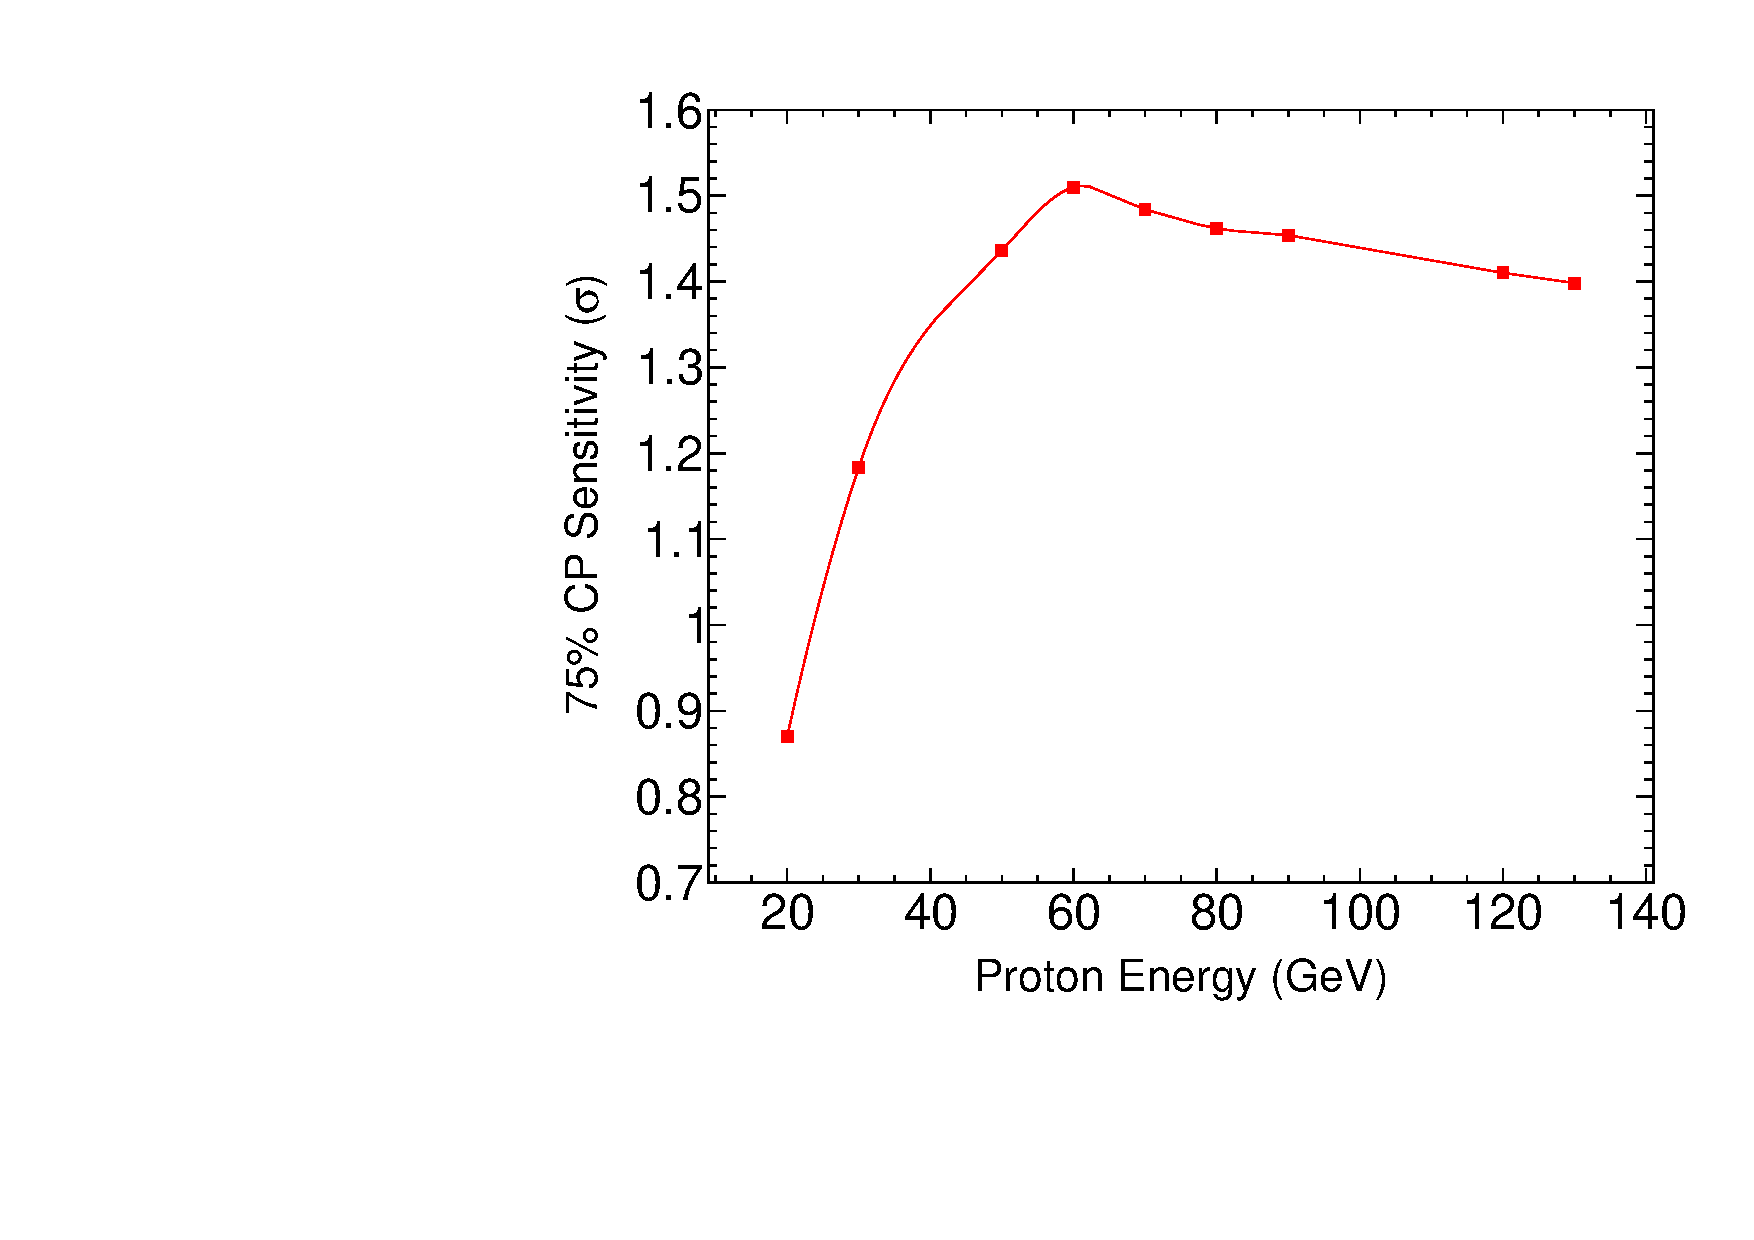
\includegraphics[width=1.0\textwidth]{summary_rp_nh_cp_75thpercentile}
\end{minipage}
\end{cdrfigure}

\begin{cdrfigure}[Neutrino flux comparison for various target 
  positions and decay pipe lengths.] {beam_req_lemehe}{Neutrino fluxes for the 
    reference beam design with 120 GeV/c protons, with the target starting 45 (LE), 135 (ME) 
    and 250 (LE) cm upstream from the start of Horn 1 (left), and the 
   fractional improvement in flux for the same beam configurations 
    when the decay pipe is lengthened to 250 m (right). {\it This 
      figure was generated with 200 kA horn current and will be 
      updated to use the new reference value of 230 kA.}}
    \includegraphics[width=0.75\textwidth]{LEMEHEComp}
  \end{cdrfigure}

\subsection{Improved Beam Options}
\label{sec:alternative-focusing-systems}

There are several potential modifications to the reference beam design that would improve the experiment's sensitivity to the CP violating phase and mass hierarchy. 
One option, which we will call enhanced reference beam, is based on 
the NuMI focusing horn design but uses a thinner and shorter 
cylindrical beryllium target positioned 25 cm upstream of the first 
focusing horn. We consider two decay pipe configurations for this 
enhanced reference beam, one 204 m long and 6 m in diameter and the other 
250 m long and 4 meters in diameter.  The neutrino fluxes for these 
options, generated with an 80 GeV/c primary proton beam, are shown in 
Figure~\ref{fig:beam_req_focusing_comp}. 
  
The option offering the largest gains in sensitivity is a redesign of the focusing system, including target and horns, which would require a modification of the dimensions 
of the present target chase.  To identify optimal designs, a genetic algorithm has been implemented to search for beam configurations that maximize sensitivity to CP violation. 
The procedure is inspired by a similar one developed by the LBNO collaboration~\cite{Agarwalla:2014tca}, and considers 20 beamline parameters governing the primary proton energy, target dimensions, 
and horn shapes, positions and current. Figure~\ref{fig:beam_req_opthorn} shows the shape and the relative parameters used for the optimization of the first focusing horn, 
while the second focusing horn is modeled as a NuMI-style horn, but allowed to rescale both in radial and longitudinal dimensions. The procedure yields horn size and shapes 
similar to those found by the LBNO collaboration. The first focusing horn is $\sim 5.5$ m in length and $\sim 1.3$ m in diameter. This 
optimized beam configuration includes a second focusing horn that is 32\% longer and 7.8 m further downstream than that of the reference focusing design.  This option would 
require an increase both in length, by $\sim 9$ m, and in width, by 
$\sim 60$ cm, of the target chase in the reference design.  Figure~\ref{fig:beam_req_focusing_comp} shows a comparison of fluxes 
for the reference, enhanced reference and optimized beam configurations. This
optimized beam, with a decay pipe 204 m long and 4 m in diameter,
produces a muon neutrino flux that is 20\% greater than the nominal
configuration at the first oscillation maximum (between 1.5 and 4 GeV), 
53\% greater at the second oscillation maximum (between 0.5 and 1.5 GeV), and reduces the
antineutrino contamination of the beam.   Sensitivity to $\delta_{CP}$ and the mass hierarchy as 
a function of the exposure for reference and alternative beam options
are shown in Figure~\ref{fig:beam_req_sensitivities}.  The optimized beam leads to improvements in sensitivity to both mass hierarchy 
and CP violation. Refinement of the optimization procedure, including
verification of the results with alternate hadron production models, and evaluation of the feasibility of the optimized designs are in progress. 

\begin{cdrfigure}[Neutrino fluxes with alternative beam designs]
{beam_req_focusing_comp}{Neutrino mode muon 
    neutrino fluxes for several beam designs, including the 
    reference, the enhanced reference, and the optimized beam
    described in section~\ref{sec:alternative-focusing-systems}.  All
    beams use 80 GeV protons.}
  \includegraphics[width=0.66\textwidth]{BeamOptCDR}
\end{cdrfigure}

\begin{cdrfigure}[Radial view of the first horn shape considered in focusing system 
  optimization]{beam_req_opthorn}{First focusing horn design considered 
    in the alternative focusing optimization. 
%\bf{To be replaced with a  better drawing}
}
  \includegraphics[width=0.75\textwidth]{horn1}
\end{cdrfigure}

\begin{cdrfigure}[Sensitivities to the mass hierarchy and
  $\delta_{CP}$ for reference and alternative beam designs]
{beam_req_sensitivities}{Sensitivity to the mass hierarchy (left) and
  $\delta_{CP}$ (right) as a function of exposure for the reference beam and
  the beam options discussed in
  Section~\ref{sec:alternative-focusing-systems}.  All beams use 80
  GeV protons.}

\centering 
\begin{minipage}{0.5\textwidth}
\centering 
\includegraphics[width=1.0\textwidth]{mh_comparebeams}
\end{minipage}\hfill 
\begin{minipage}{0.5\textwidth}
\centering 
\includegraphics[width=1.0\textwidth]{cpv75_comparebeams}
\end{minipage} 
\end{cdrfigure}

\section{Detector Requirements}
\label{sec:physics-lbnosc-det-req}

\subsection{Far Detector Requirements}
\label{sec:physics-lbnosc-fd-req}

The DUNE Far Detector (FD) requirements relevant to long-baseline neutrino oscillation physics include:
\begin{itemize}
 \item Identification of Electron Neutrino and Antineutrino Events: The FD shall be capable of identifying electron neutrino and antineutrino charged current beam events in sufficient numbers within the fiducial volume of the detector. The neutrino flavor of the event will be identified by clearly identifying the primary final state charged electron. The total energy of the charged current event shall be measured. 
 \item Muon Neutrino and Antineutrino Events: The FD shall be capable of identifying muon neutrino and antineutrino charged current beam events in sufficient numbers within the fiducial volume of the detector and identify the primary muon particle emerging from the main event vertex.  The total energy of the charged current event shall be measured. 
 \item Multiple tracks and Electromagnetic Showers: The FD shall be capable of identifying events with multiple electromagnetic showers and non-showering particles produced within the fiducial volume of the detector.
 \item Baseline Length: A baseline of sufficient length shall be established between the neutrino beam facility and a far detector facility so that the difference between muon to electron neutrino conversion for the two cases of neutrino mass ordering can be clearly separated from the variation due to the CP phase, leading to unique determination of the CP phase.
 \item  Cosmic Ray Shielding: The FD shall be located at a depth to reduce the number of in-time (within the beam spill time) cosmic ray background so that it does not contribute more than 1\% of the final beam neutrino sample. 
 \item CP Phase Measurement: The total number of observed electron-neutrino and electron-antineutrino type events -- including consideration of background -- shall be sufficient to measure the CP phase to better than 3 sigma at the maximum CP violation. 
 \item Time Accuracy: Individual event times shall be measured with sufficient time accuracy to allow correlation of event times between detectors that are geographically separated. In the case of long-baseline oscillations, this would include correlation between the DUNE near and far detectors.  
\end{itemize}


\subsection{Near Detector Requirements}
\label{sec:physics-lbnosc-nd-req}

The DUNE Near Detector (ND) requirements relevant to long-baseline neutrino oscillation physics include:
\begin{itemize}
 \item FD measurements not limited by ND: ND measurements shall be of sufficient precision to ensure that when extrapolated to FD to predict the FD event spectra without oscillations, the associated systematic error must be significantly less than the statistical error over the lifetime of the experiment. 
 \item Muon Neutrino and Antineutrino Flux measurements: The ND shall measure the absolute and relative muon neutrino and antineutrino spectra separately.
 \item Electron Neutrino and Antineutrino Flux measurements: The ND shall measure the electron-neutrino and antineutrino contamination spectra of the beam separately in order to render the CP measurement as precise as possible.
 \item Background Measurements: The ND shall measure rates, kinematic distributions and detailed topologies of physics processes that could mimic signal events in the FD nuclear targets. This measurement shall be made with sufficient resolution to allow FD background calculation with precision that does not limit the oscillation measurements.
 \item Cross section measurements I: The ND will measure CC and NC cross sections separately as a function of hadronic energy.
 \item Cross section measurements II: The ND shall characterize various exclusive and semi-exclusive processes such as quasi-elastic interactions, resonance production, deep inelastic scattering, and neutrino-electron and neutrino-proton elastic scattering.
 \item Cross section measurements III: The ND shall measure the neutrino nucleus cross section off various targets like Hydrogen, Ar, Fe, Ca, and C.
\end{itemize}

\section{Effect of Systematic Uncertainties}
\label{sec:physics-lbnosc-beamnd-req}
Sensitivity studies presented in Section~\ref{sec:physics-lbnosc-senscalc} test the ability to distinguish
the expected number of \nue appearance and \numu disappearance events given a set of oscillation parameters
from the expectations given an alternate set of parameters. For example, the CP violation and MH sensitivity
studies test the spectral differences induced by shifting \deltacp away from 0.0 and $\pi$ and by changing the
mass hierarchy. These difference are quantifyed with a test statistic (see Eq.~\ref{eq:dx2_MH}~-~\ref{eq:dx2_CP}) 
which accounts for statistical and systematic uncertainties. 
The effect of systematic uncertainty in the underlying models parameters used to 
predict these spectra is included by allowing the paramaters to vary within gaussian ranges. In the fit
these systematic nuisance parameters are profiled, i.e. the set of nuisance parameters that produces the
lowest total value of the test statistic is chosen.  The central values and 1$\sigma$ uncertainties on the oscillation
parameters are taken from the Nu-Fit~\cite{Gonzalez-Garcia:2014bfa} global fit to neutrino data; the values are
given in Table~\ref{tab:oscpar_nufit}. Uncertainty in the non-oscillation parameters is approximated using
normalization uncertainties on each constituent interaction mode that comprise the signal and background
interactions in each sample. These normalization uncertainties are chosen based on
current constraints on underlying model parameters, the ability of previous experiments to constrain
these quantities, and the expected ability of the DUNE Near Detector (ND) as outlined in Section~\ref{reftoND}.
Consideration is also given to the sources of uncertainty that go into each of the effective normalization
parameters and how they may be correlated among the Far Detector (FD) analysis samples that will be fit in
combination.

%In the sensitivities presented in Section ~\ref{sec:physics-lbnosc-senscalc},
%the \nue and \anue signal normalization uncertainties are $5\% \oplus 2\%$, implemented as
%5\% signal normalization uncertainties on the \numu and \anumu samples and
%2\% on the \nue and \anue samples. These four signal normalization uncertainties
%are treated as 100\% uncorrelated so that the 2\% normalization uncertainty on the
%\nue sample represents a residual normalization uncertainty after constraints
%from the near detector, the \numu disappearance samples, and the \anue sample have been applied.
%The normalization uncertainties on background to these samples and the correlation among those
%uncertainties are presented in Table~\ref{tab:bgnormsys}. The result of the correlations
%described in Table~\ref{tab:bgnormsys} is that there are five independent background
%normalization uncertainties: beam \nue, beam \anue, \numu/NC background to appearance mode,
%NC background to disappearance mode, and $\nu_\tau$. 

\begin{table}[!tb]
  \begin{center}
    \caption{Normalization uncertainties and correlations for background to the \nue, \anue, \numu, and \anumu data samples.}
    \label{tab:bgnormsys}
    \begin{tabular}{l|c|l} \hline\hline
      Background & Normalization Uncertainty & Correlations \\ \hline
      \multicolumn{3}{l}{For \nue/\anue appearance:} \\ 
      Beam \nue & 5\% & Uncorrelated in \nue and \anue samples \\
      NC      & 5\%  & Correlated in \nue and \anue samples \\
      \numu CC & 5\% & Correlated to NC \\
      $\nu_\tau$ CC & 20\% & Correlated in \nue and \anue samples \\ \hline
      \multicolumn{3}{l}{For \numu/\anumu disappearance:} \\ 
      NC & 5\% & Uncorrelated to \nue/\anue NC background \\
      $\nu_\tau$ & 20\% & Correlated to \nue/\anue $\nu_\tau$ background \\
    \end{tabular}
  \end{center}
  \end{table}

In the following sections, we present a justification for the chosen values of the signal and background
normalization uncertainties and thier respective correlations.
Studies that consider the effect of varying the size of the residual normalization
uncertainties on the \nue and \anue samples are also presented.
Finally we describe the ongoing effort to characterize and evaluate the effect of individual sources
of uncertainty when propagated to oscillation parameter measurments in the DUNE experiment.

\subsection{Effective Normalization Parameters and Correlations}
\label{sec:syst_just}
Uncertainties in DUNE will be constrained by external data, near detector data, and the combined
fit to the four (\nue appearance, \anue appearance, \numu disappearance, \anumu disappearance) far detector samples.
The \numu disappearance analysis sample is composed of \numu CC interactions with backgrounds from NC
interactions in which a charged pion is misidentified a muon and $\nu_{\tau}$ CC interactions in which the resulting
tau decays to a muon and two neutrinos.
The unoscillated \numu flux and related cross sections are expected to be well-constrained by the near detector.
The uncertainty on the neutral current background comes primarily from uncertainty in pion production rates
for the coherent, resonance and DIS channels, as well as the modelling pion fates which determine the 
if the topological signature of the pion is consistent with that of a muon. 
%The charged pion misidentification rate, and its associated
%uncertainty, is highly correlated with the fraction
%of pions that either exit the detector, are absorbed by nuclei, or expend their kinetic before interacting
%hadronically, and thus have the topological characteristics of a muon.
%These relative rates of these processes will be constrained by the ND.
Uncertainties in the $\nu_{\tau}$ CC background level arise from the uncertainty in the $\nu_{\tau}$/\numu
cross-section ratio, which cannot be constrained by ND measurements. Each of these three samples are
assigned a normalization unceratainty. 

The \nue appearance sample is composed of electron neutrinos resulting from \numu$\rightarrow$\nue oscillation,
intrinsic beam \nue, NC and high-y$_{bj}$ \numu CC interactions in which a photon from a final-state neutral pion is
misidentified as an electron, and $\nu_{\tau}$ interactions in which the tau decays to an electron and
two neutrinos. Since the
\numu disappearance signal and the \nue appearance signal are produced by the same flux
%, flux uncertainty is constrained in the three-flavor fit.
%For example, changing the flux will increase the relative rates of the numu and nue samples the amount,
%while adjusting q23 will cause one sample to rise and the other to fall.
the \nue appearance signal is constrained relative to the \numu
signal. The residual uncorrelated uncertainty on the \nue signal results from the statistical limits of the \numu sample
constraint, differences in energy scale and selection efficiency between the samples,
as well as theoretical uncertainties on the \nue/\numu cross-section ratio. These contribution are summed
quadratically and are assigned to the \nue signal normalization parameter uncertainty. 

The uncertainty on the intrinsic
beam \nue background is dominated by flux uncertainties which are constrained by the near detector.
Predictions for neutral current and \numu CC background rates are again limited by the uncertainties on pion
production rates, and the uncertainty assigned to the normalization parameter for the \nue appearance sample combines uncertaintes
on the $\pi^{0}/\pi^{\pm}$ production ratio, and differences in detection and selection efficiencies.
%There are correlations between the charged and neutral pion production rates, allowing for
%cancellation of uncertainty in this background between the \nue and \numu samples.
%However, to be conservative the NC+CCnumu backgrounds in the nue are allowed to vary by an additional
%uncorrelated 5% to account for differences in pi0/pi+- production rates, and detection/selection efficiencies.
The $\nu_{\tau}$ background uncertainties are again related to cross-section ratio uncertainties
which are 100\% correlated among samples.

Energy scale uncertainties, which can affect the shape of the reconstructed energy spectra, result from
inaccurate models of detector response, missing energy in the hadronic systems (primarily from neutron production),
and from FSI. Since the dominant source of uncertainty is the hadronic energy scale which is the same for both
signal samples, the relative energy scale uncertainties are limited to differences in kinematics
between \numu and \nue interactions and differences in detector response for muons and electrons,
which will be highly constrained by test beam experiments.

The effectice normalization parameters for the antineutrino (RHC) beam \nue and \numu samples mirror the
those described above for the neutrino (FHC) beam samples.
Additional constraints are expected to occur in a fit to both neutrino and antineutrino beam samples;
variations in \deltacp induce opposite effects (in both shape and rate) in the \nue and \anue samples,
while most systematic uncertainties have a positively correlated effect. Notable correlation considerations between
the FHC and RHC samples include: signal and beam \nue background parameters are uncorrelated, 
\numu and \anumu NC backgrounds are 100\% correllated with eacheaother, as are \nue and \anue
NC and \numu CC backgrounds. The normalization parameters fo the \nutau CC backgrounds are all 100\% correlated.

%% Similar arguments can be made for the antineutrino (RHC) beam samples, and therefore the same effective normalization uncertainties are used. The choice of uncertainties on the effective normalization parameters also reflect the significant cancellations achieved in the 4-sample fit resulting from the addition of 1) relating the nuebar app samples to the numubar dis samples, and 2) from the fact that variations in dcp induce opposite effects (in both shape and rate) in nue and nuebar samples, while most systematics have a positively correlated effect. In these choices it is conservatively assumed that the nu (FHC) flux and the nubar (RHC) flux are not correlated. The only systematic thought to be able to induce an anti-symmetric response between the nue and nuebar samples comes from FSIs. This will require careful constraint from ND analysis, external data, and comparisons of nue to numu, and nuebar to numubar, where the peak of the appearance and the trough of the disappearance samples must be the same. 

Energy scale uncertainties, which can affect the shape of the reconstructed energy spectra, result from
inaccurate models of detector response, missing energy in the hadronic systems (primarily from neutron production),
and from FSI. Since the dominant source of uncertainty is the hadronic energy scale which is the same for both
signal samples, the relative energy scale uncertainties are limited to differences in kinematics
between \numu and \nue interactions and differences in detector response for muons and electrons,
which will be highly constrained by test beam experiments.

Systematic uncertainties stemming from the FSI model are thought to be able to induce an anti-correlated 
energy scale differences between the \nu and \anu samples. This has the potential to mimic the effects
of a non-zero or \pi value of \deltacp. The effect will however be the same in the \nue (\anue) and \numu
(\anumu) samples allowing the relative \nue/\numu (\anue/\anumu) energy scale to be fixed by comparing
the peak of the appearance and the trough of the disappearance spectra. Additional constraints on the FSI 
model will required from ND analyses, and external data.


%Based on these considerations and experience from previous and currently-running neutrino oscillation 
%experiments, we believe that $5\% \oplus 2\%$ signal normalization (where 5\% is the normalization uncertainty on the
%FD \numu sample and 2\% is the effective uncorrelated uncertainty on the FD \nue sample after fits to both near
%and FD detector data and all external constraints) and normalization uncertainties on background as given
%in Table \ref{tab:bgnormsys} are reasonably achievable in DUNE given a capable near detector with argon targets.
%Table~\ref{tab:nuesysts} shows the uncertainties in a \nue appearance analysis achieved by MINOS~\cite{Adamson:2013ue} 
%and T2K~\cite{Abe:2015awa} and compares the expected uncertainty in
%DUNE. The goal uncertainties in DUNE are chosen by determining which
%of the existing experiments is more representative of DUNE for each source
%of systematic uncertainty and then setting a reasonable goal for a next-generation
%experiment. These goals are based on the expected capabilities of the high-resolution
%LAr TPC and  precise measurements from a highly-capable near detector, as well as
%understanding of the analysis techniques employed by previous experiments.
%A brief explanation of each choice in Table~\ref{tab:nuesysts} follows.
%
%\begin{table}[!hb]
%\begin{center}
%  \caption {The dominant systematic uncertainties on the $\nu_e$-appearance 
%    signal prediction in MINOS and T2K and a conservative projection of the 
%    expected uncertainties in DUNE. In each case, the quoted uncertainty is
%    the effect on the $\nu_e$-appearance signal only. These uncertainties 
%    are the \emph{total} expected uncertainties on the $\nu_e$-appearance signal 
%    which include both correlated and uncorrelated uncertainties in the 
%    three-flavor fit. For reference, the uncertainties assumed in the nominal
%    DUNE sensitivity calculations are also provided.\vspace{2pt}}
%\label{tab:nuesysts}
%\begin{tabular}{|l|c|c|c|l|} \hline\hline
%Source of & MINOS & T2K & DUNE & Comments \\ \hline\hline
%\multicolumn{5}{|c|}{Flux}  \\ \hline
%Uncertainty & $\nu_e$ & $\nu_e$ & $\nu_e$ & \\ \hline\hline
%Beam Flux & 0.3\% & 3.2\% & 2\% & See ``Flux Uncertainties'' in Section \ref{sec:syst_just_flux}\\
%after N/F & & & & \\
%extrapolation & & & & \\ \hline\hline
%\multicolumn{5}{|c|}{Neutrino interaction modeling}  \\ \hline
%Simulation & 2.7\% & 4.7\% & $\sim 2\%$ & See ``Simulation Uncertainties'' in Section \ref{sec:syst_just_sim} \\
%includes: & & & & \\
%hadronization & & & &  \\ 
%cross sections & & & & \\ 
%nuclear models & & & & \\ 
%& & & & \\ \hline\hline
%\multicolumn{5}{|c|}{Detector effects}  \\ \hline
%Energy scale  & 3.5\% & included& (2\%) & Included in 5\% $\nu_\mu$ sample\\ 
%($\nu_\mu$) & & above & &  normalization uncertainty in DUNE 3-flavor fit. \\ \hline
%Energy  scale & 2.7\% & 2.5\% & 2\% & See ``\nue Energy Scale Uncertainties''\\
%($\nu_e$) & & includes & &  in Section\ref{sec:syst_just_fd}\\
% & & all FD & & \\
% & & effects & & \\ \hline 
%Fiducial & 2.4\% & 1\% & 1\% & Larger detectors = smaller uncertainty. \\ 
%volume & & & & \\ \hline\hline
%Total  & 5.7\% & 6.8\% & 3.6 \% & Residual $\nu_e$ uncertainty in  \\ 
%& & & & full DUNE 3-flavor fit = 1-2\%. \\ \hline\hline
%Used in DUNE & & & $5\% \oplus 2\%$ & 2\% \\
%Sensitivity & & & & \\
%Calculations & & & & \\ \hline \hline
%\end{tabular}
%\end{center}
%\end{table}

\subsection{Projecting Unceratinties Based on Previous Experience}

Table~\ref{tab:nuesysts} shows the uncertainties in a \nue appearance analysis achieved by MINOS~\cite{Adamson:2013ue}
and T2K~\cite{Abe:2015awa} and compares the expected uncertainty in
DUNE. The goal uncertainties in DUNE are chosen by determining which
of the existing experiments is more representative of DUNE for each source
of systematic uncertainty and then setting a reasonable goal for a next-generation
experiment. These goals are based on the expected capabilities of the high-resolution
LAr TPC and  precise measurements from a highly-capable near detector, as well as
understanding of the analysis techniques employed by previous experiments.
A brief explanation of each choice is also shown in Table~\ref{tab:nuesysts},
while more detailed explainations are given below.


\subsubsection{Flux Uncertainties}
\label{sec:syst_just_flux}
DUNE plans to take advantage of spectral analysis,
meaning that absolute and relative flux normalization is required. Since the MINOS \nue appearance analysis
is based on normalization only, in terms of the \nue appearance analysis, DUNE will be more like T2K,
which has achieved 3.2\% normalization uncertainty on their \nue sample due to flux. Additionally, for a more apt
comparison to MINOS performance, the inclusive neutrino charged current cross-section measurement from the MINOS
near detector reported in \cite{xxx} has acheived a normalization uncertainty of $\sim$2\% in the
range $3 < E_\nu < 9$ GeV and the near-to-far \numu unoscillated-spectrum extraplolation errors in MINOS
are $<$3\% without any independent constraints on hadron production or muon flux measurements at the near
site. Therefore, as DUNE is planned to have a highly capable near detector, beam line
muon detectors, dedicated hadronization measurements, and improved simulation of beam flux based on MINERvA
measurements in the NuMI beam, we set a goal uncertainty on \nue signal
normalization from uncertainties in the flux determination of 2\%.
As described in Section \ref{sec:syst_studies_ind}, preliminary
studies of the FGT ND support this estimate, predicting 2\% uncertainty on the absolute flux and 1-2\%
uncertainty on the flux shape.
\subsubsection{Simulation Uncertainties}
\label{sec:syst_just_sim}
This category of uncertainties arise primarily from uncertainties in modeling neutrino interactions with the target
nuclei in the near and far detectors. These uncertainties include \nue and \numu cross-section uncertainties,
uncertainties from modeling the structure of the target nucleus, and the impact of
hadronization model uncertainties in simulating the break up of the target nucleus in higher-energy inelastic
interactions. DUNE will employ argon nuclear targets in both the near and far detectors, allowing for a larger
cancellation of simulation uncertainties than in T2K, in which the target nuclei in the near detector are
carbon while those in the far detector are oxygen. Additionally, the angular resolution, vertex resolution,
and particle identification capability of the DUNE near detector are expected to increase its ability to
constrain those cross-section uncertainties which are common between near and far detectors, but for which
the T2K near detector could not provide significant constraint.
Finally, DUNE's high-resolution near
detector is expected to enable further constraints on hadronization uncertainties, relative to MINOS, by
resolving many of the individual particles produced in the resonance and deep-inelastic scattering interactions
which represent the majority of the DUNE data sample. Therefore, we take 2\% as a goal for the effect of
simulation uncertainties on DUNE \nue signal normalization. It is important to note that this level of
uncertainty depends upon the ability to isolate neutrino-argon interactions in the near detector to facilitate
cancellation of near-far uncertainties; this is a requirement of the ND design.

Additionally, in considering the effect of the three-flavor analysis on the final uncertainty,
the neutrino beams in DUNE and MINOS have energy
spectra that peak around 2.5-3.0~GeV, compared to 600~MeV in T2K. The impact of the inability to
constrain the ratio of \nue/\numu cross-sections in T2K will be significantly reduced in DUNE
where the energy range is higher and the theoretical limits on the cross-section differences is
well within 1\%~\cite{DanSaidSo}. This constraint increases
the level of cancellation that can be expected in the three-flavor analysis. As
described in Section~\ref{sec:syst_studies_ind}, preliminary studies with a Fast MC demonstrate the
expected cancellation of cross-section uncertainties in the DUNE three-flavor analysis.

\subsubsection{\nue Energy Scale Uncertainties}
\label{sec:syst_just_fd}
MINOS and T2K have acheived uncertainty in the \nue signal normalization from \nue energy scale
of 2.7\% and 2.5\% respectively,
where the 2.5\% from T2K actually includes most far detector effects. DUNE's LAr TPC far detector
is expected to outperform both the MINOS sampling calorimeter and the T2K water Cerenkov detector
in reconstruction of \nue interactions. Purity of the quasielastic-like event selection
should be improved relative to T2K by the capability of the LAr TPC to detect hadronic showers
that would be below threshold in SuperK, as described in \cite{UlrichMosel}. For non-quasielastic-like
events, the low thresholds and high resolution of the DUNE LAr TPC will significantly improve
calorimetric reconstruction over the MINOS sampling calorimeter.
Significant experience with simulation, reconstruction, and calibration
of neutrino interactions in LAr TPCs is expected from the Intermediate Neutrino Program, particularly
Fermilab's SBN program which will include three LAr TPCs: SBND, $\mu$BooNE, and ICARUS. An active program of
prototypes and test beam measurements is planned to study the reconstruction of charged and neutral particles
in LAr TPCs; this suite of experiments includes the DUNE 35-ton prototype, LArIAT, CAPTAIN, and
the CERN neutrino platform single and dual phase prototypes.
Therefore, we set a goal of using the superior detector performance and the improvments
in understanding of LAr TPC energy response expected in the next 5-10 years to reduce the normalization uncertainty
from the \nue energy scale to 2\%.

In considering the effect of the three-flavor analysis on the final uncertainty, hadronic energy is expected
to contribute more than half of the total energy deposit for many \nue and \numu interactions in the DUNE
far detector. Since the hadronic energy scale does not depend on neutrino flavor, the uncertainties on this
portion of the LAr TPC energy response are expected to largely cancel in the DUNE three-flavor analysis, up
to kinematic differences in the \nue and \numu samples. The samples in the three-flavor fit, particularly the
neutrino and antineutrino samples, will have significantly different contributions from neutrons, so understanding
of neutron production and detector response will be important for cancellation of uncertainty in this fit.
Deployment of the CAPTAIN detector in a neutron beam at LANL is planned to address these issues.

\subsection{Normalization Paramter Uncertainties}

Table~\ref{tab:nuesysts} shows the uncertainties in a \nue appearance analysis achieved by MINOS~\cite{Adamson:2013ue}
and T2K~\cite{Abe:2015awa} and compares the expected uncertainty in
DUNE. The goal uncertainties in DUNE are chosen by determining which
of the existing experiments is more representative of DUNE for each source
of systematic uncertainty and then setting a reasonable goal for a next-generation
experiment. These goals are based on the expected capabilities of the high-resolution
LAr TPC and  precise measurements from a highly-capable near detector, as well as
understanding of the analysis techniques employed by previous experiments.
A brief explanation of each choice in Table~\ref{tab:nuesysts} follows.

Based on the considerations of the sources of systematic uncertainty 
and experience from previous and currently-running neutrino oscillation
experiments, we believe that $5\% \oplus 2\%$ signal normalization (where 5\% is the normalization uncertainty on the
FD \numu sample and 2\% is the effective uncorrelated uncertainty on the FD \nue sample after fits to both near
and FD detector data and all external constraints) and normalization uncertainties on background as given
in Table \ref{tab:bgnormsys} are reasonably achievable in DUNE given a capable near detector with argon targets.
The goal for the \emph{total} uncertainty on the \nue sample in
DUNE is less than 4\%, so the $5\% \oplus 2\%$ \nue signal normalization uncertainty
used for the sensitivity calculations is appropriately conservative.
Additionally, significant cancellation of uncertainty is expected in the four-sample fit, so the
residual uncorrelated normalization uncertainty on the \nue sample is expected to be reduced to the 1-2\% level,
such that the 2\% residual normalization uncertainty portion of the uncertainties in the sensitivity calculations
is also well-justified.
%
\begin{table}[!hb]
\begin{center}
  \caption {The dominant systematic uncertainties on the $\nu_e$-appearance
    signal prediction in MINOS and T2K and a conservative projection of the
    expected uncertainties in DUNE. In each case, the quoted uncertainty is
    the effect on the $\nu_e$-appearance signal only. These uncertainties
    are the \emph{total} expected uncertainties on the $\nu_e$-appearance signal
    which include both correlated and uncorrelated uncertainties in the
    three-flavor fit. For reference, the uncertainties assumed in the nominal
    DUNE sensitivity calculations are also provided.\vspace{2pt}}
\label{tab:nuesysts}
\begin{tabular}{|l|c|c|c|l|} \hline\hline
Source of & MINOS & T2K & DUNE & Comments \\ \hline\hline
\multicolumn{5}{|c|}{Flux}  \\ \hline
Uncertainty & $\nu_e$ & $\nu_e$ & $\nu_e$ & \\ \hline\hline
Beam Flux & 0.3\% & 3.2\% & 2\% & See ``Flux Uncertainties'' in Section \ref{sec:syst_just_flux}\\
after N/F & & & & \\
extrapolation & & & & \\ \hline\hline
\multicolumn{5}{|c|}{Neutrino interaction modeling}  \\ \hline
Simulation & 2.7\% & 4.7\% & $\sim 2\%$ & See ``Simulation Uncertainties'' in Section \ref{sec:syst_just_sim} \\
includes: & & & & \\
hadronization & & & &  \\
cross sections & & & & \\
nuclear models & & & & \\
& & & & \\ \hline\hline
\multicolumn{5}{|c|}{Detector effects}  \\ \hline
Energy scale  & 3.5\% & included& (2\%) & Included in 5\% $\nu_\mu$ sample\\
($\nu_\mu$) & & above & &  normalization uncertainty in DUNE 3-flavor fit. \\ \hline
Energy  scale & 2.7\% & 2.5\% & 2\% & See ``\nue Energy Scale Uncertainties''\\
($\nu_e$) & & includes & &  in Section\ref{sec:syst_just_fd}\\
 & & all FD & & \\
 & & effects & & \\ \hline
Fiducial & 2.4\% & 1\% & 1\% & Larger detectors = smaller uncertainty. \\
volume & & & & \\ \hline\hline
Total  & 5.7\% & 6.8\% & 3.6 \% & Residual $\nu_e$ uncertainty in  \\
& & & & full DUNE 3-flavor fit = 1-2\%. \\ \hline\hline
Used in DUNE & & & $5\% \oplus 2\%$ & 2\% \\
Sensitivity & & & & \\
Calculations & & & & \\ \hline \hline
\end{tabular}
\end{center}
\end{table}

These assumptions for the non-oscillation systematic uncertainties 
are used to calculated sensitivities presented in Section ~\ref{sec:physics-lbnosc-senscalc}.
Variations on these assumptions are explored in the next subsection.

\subsection{Effect of Normalization Uncertainties}
Figure \ref{fig:exp_systs} shows the
change in DUNE sensitivity to determination of
neutrino mass hierarchy and discovery of CP violation
as a function of exposure for several levels of signal normalization uncertainty.
As seen in Fig.~\ref{fig:exp_systs}, for early phases of DUNE
with exposures less than 100 kt-MW-years, the experiment
will be statistically limited. In the full experiment, signal and
background normalization uncertainties remain
relatively unimportant for the mass hierarchy measurement, when considering
minimum sensitivity for 100\% of \deltacp values, because the minimum sensitivity 
occurs in the near-degenerate region where it becomes difficult to determine
whether one is observing \deltacp $= + \pi/2 $ in the normal hierarchy
or \deltacp $=-\pi/2$ in the inverted hierarchy. Spectral analysis will
help resolve this near-degeneracy, but is dependent on as-yet
unexplored uncertainties in the spectral shape, which are expected to be dominated
by energy-scale uncertainty. Studies of these effects are in progress and will be included in
future analyses of experimental sensitivity; Figure~\ref{fig:escale_syst} shows the
impact on MH and CP violation sensitivity of one possible energy scale variation.
\begin{figure}[!htbp]
\centering
\includegraphics[width=0.32\linewidth]{volume-physics/figures/mh_exp_syst.pdf}
\includegraphics[width=0.32\linewidth]{volume-physics/figures/cpv50_exp_syst.pdf}
\includegraphics[width=0.32\linewidth]{volume-physics/figures/cpv75_exp_syst.pdf}
\caption{Expected sensitivity of DUNE to determination of the neutrino mass
  hierarchy (left) and discovery of CP violation, i.e. $\delta_{CP} \ne$ 0 or $\pi$,
  (middle, right) as a function of exposure in kt-MW-years, assuming 
  equal running in neutrino and antineutrino mode, for a range of values for
  the \nue and \anue signal normalization uncertainties from $5\%\oplus3\%$ to
  $5\%\oplus1\%$. The sensitivities quoted
  are the minimum sensitivity for 100\% of \deltacp values in the case of 
  mass hierarchy and 50\% of \deltacp values (middle) or 75\% of \deltacp values (right)
  in the case of CP violation. The two bands on each plot represent a range of potential
  beam designs: the blue hashed band is for the CDR Reference Design and the solid green
  band is for the Optimized Design. 
  Sensitivities are for true normal hierarchy; neutrino mass hierarchy
  and $\theta_{23}$ octant are assumed to be unknown.}
\label{fig:exp_systs}
\end{figure}
%
%% \begin{figure}[!htbp]
%% \centering
%% \includegraphics[width=0.32\linewidth]{volume-physics/figures/
%% \includegraphics[width=0.32\linewidth]{volume-physics/figures/
%% \includegraphics[width=0.32\linewidth]{volume-physics/figures/
%% \caption{Expected sensitivity of DUNE to determination of the neutrino mass
%%   hierarchy (left) and discovery of CP violation, i.e. $\delta_{CP} \ne$ 0 or $\pi$,
%%   (middle, right) as a function of exposure in kt-MW-years, assuming 
%%   equal running in neutrino and antineutrino mode, for a range of values for
%%   the \nue and \anue signal normalization uncertainties from $5\%\oplus3\%$ to
%%   $5\%\oplus1\%$. The sensitivities quoted
%%   are the minimum sensitivity for 100\% of \deltacp values in the case of 
%%   mass hierarchy and 50\% of \deltacp values (middle) or 75\% of \deltacp values (right)
%%   in the case of CP violation. The two bands on each plot represent a range of potential
%%   beam designs: the blue hashed band is for the CDR Reference Design and the solid green
%%   band is for the Optimized Design. 
%%   Sensitivities are for true normal hierarchy; neutrino mass hierarchy
%%   and $\theta_{23}$ octant are assumed to be unknown.}
%% \label{fig:escale_systs}
%% \end{figure}

The impact of systematic uncertainty on the CP violation sensitivity
is obvious in Fig.~\ref{fig:exp_systs}; the \nue signal normalization uncertainty must
be understood at the level of $5\% \oplus 2\%$ in order to reach 5$\sigma$ sensitivity for
75\% of \deltacp values with exposures less than $\sim$900~kt-MW-years in the case of the
Optimized Design. Specifically, the absolute normalization of the \numu sample must be known to
$\sim$5\% and the normalization of the \nue sample,
relative to the \anue, \numu, and \anumu samples after all constraints from
external, near detector, and far detector data have been applied, must be determined 
at the few percent level. This level of systematic uncertainty sets the capability and
design requirements for all components of the experiment, including the beam design, and the
near and far detectors.


%
\subsection{Ongoing Studies of Detailed Systematic Uncertainties}
\label{sec:syst_studies_ind}
Detailed evaluation of systematic uncertainties for DUNE is ongoing. In many cases plans for studies
have been developed but have not yet been executed. In general, each systematic will be studied both by
propagating its uncertainty to oscillation analyses to evaluate the resultant degradation of the sensitivity
and by ensuring the varied model parameter and its allowed range gives proper coverage, i.e., truly encapsulates
the lack of knowledge of the process/effect in question. Estimates for systematics constraints for
propagation studies will be varied between current external knowledge to evaluate what would be possible in the
absence of a DUNE near detector and conservative and optimistic projections
for ND performance. In cases where systematic uncertainty is shown to degrade the oscillation parameter
measurement sensitivities, the required constraints will become detector performance requirements.
The details of these studies is beyond the scope of this document, however the conclusions from some
initial studies and an overview of each source of systematic uncertainty is laid out in the remainder of this section.

Initial studies using a Fast Monte Carlo with a parameterized detector response
predict 2-3\% statistical uncertainties on the absolute flux using fully 
leptonic neutrino interactions for which high-precision cross-section predictions 
exist. Specifically,
the statistical uncertainty is expected to be 2\% for neutrino-electron
scattering ($E_\nu<5$~GeV) and 3\% for inverse muon decay ($E_\nu>11$~GeV).
Relative normalization using the low-$\nu_0$ method is
expected to constrain the flux shape and the near/far flux ratio to 1-2\%.
Studies using a multi-sample fit  to constrain the flux with simulated near detector
event samples show significant constraints on all flux
uncertainties. The post-fit uncertainty 
in most flux bins for a preliminary fit is less
than 5\%, which is the uncorrelated \numu signal normalization
uncertainty assumed by the sensitivity calculations. 

Results from a fit to Fast MC simulation of all four far detector samples
(\nue, \anue, \numu, \anumu) significantly
constrains cross-section systematic uncertainty even in the case where many
cross-section parameters are allowed to vary simultaneously within their
GENIE uncertainties. As seen in the example shown in Figure
\ref{fig:MAresqesyst}, 
a fit in which both $M_A^{QE,CC}$ and 
$M_A^{RES,CC}$ are allowed to vary within their GENIE uncertainties 
($\pm$20\%), which could significantly alter the energy distribution of the 
the selected events, results in a dramatic reduction in sensitivity if one 
considers only the $\nu_e$ appearance signal without constraint from the 
$\bar{\nu}_e$ and $\nu_{\mu}$/$\bar{\nu}_{\mu}$ samples.
In contrast, for a four sample fit,
this same parameter variation results in only a small reduction in
sensitivity to CP violation.
This result includes a 10\% uncertainty in the $\nu/\bar{\nu}$
cross-section ratio and a 2.5\% uncertainty in the $\nu_e/\nu_{\mu}$
cross-section ratio.
Preliminary studies also
demonstrate significant constraint on cross-section systematics from the 
near detector. The validity of the GENIE model parameter uncertainties are being studied 
via comparisons with available data (e.g. MINERvA), and alternate models (e.g. the 
Intranuke intranuclear rescattering model and related uncertainties will be compared with GiBUU).
These comparisons are a high priority of the whole neutrino community as well as the DUNE collaboration.
\begin{figure}[!htbp]
\centering
\includegraphics[width=0.8\linewidth]{volume-physics/figures/CPV_MARESQE.png}
\caption{An example CP violation sensitivity calculated using inputs from the 
  FastMC in a fit to all four ($\nu_e$, $\overline\nu_e$, $\nu_{\mu}$, 
  $\overline\nu_{\mu}$) samples (red) and a fit to the $\nu_e$ appearance sample 
  only (blue), for the case of no systematic uncertainty (solid) and the case in
  which both $M_A^{QE,CC}$ and $M_A^{RES,CC}$ are allowed to vary with a
  1$\sigma$ uncertainty of 20\% (dashed). This example was taken from an earlier
  DUNE study, so the absolute sensitivity can not be compared with the DUNE 
  sensitivities presented in this document.}
\label{fig:MAresqesyst}
\end{figure}

Uncertainty stemming from simulations of the interactions between hadrons
exiting the primary interaction vertex and the nuclear medium, and detector effects
such as resolutions and energy scale uncertainty, are somewhat more difficult to address with early
simulation efforts. However, in analogy to the treatment of cross-section uncertainty described above,
the effect of varying nuclear interaction parameters within their GENIE
uncertainties and comparisons of GENIE predictions to those of other
event generators are in progress.
Efforts to improve modeling of nuclear interactions and to develop 
reconstruction and analysis tools for a full Monte Carlo simulation are also underway. 
At the same time,
a number of test-beam and prototype experiments, including the DUNE 35-t prototype,
LARIAT, CAPTAIN, and the CERN neutrino platform experiments, are being designed and built to reduce these
uncertainties with experimental data.

The two main sources of uncertainty in the beam simulation come from variations in the beam optics
($\mathcal{O}$(1\%)) and uncertainties in the hadron production models ($\mathcal{O}$(10\%)).
Beam optics have been studied in detail, and while the variations in the flux produced by these uncertainties
lead to large uncertainties in the FD-only fits, they are easily constrained by the ND. Software tools that
allow reweighting of neutrinos based on their parent hadrons have been developed by MINERvA; we are working with
them port those tools to DUNE. In the meantime MINERva has agreed to provide their flux covariance matrix
that details the flux rate and shape uncertainties prior to ND constraints. We will combine this with DUNE
simulations to project reasonable hadron production uncertainties to ND and FD analyses.

Each cross section model has uncertainties. In most cases these come from the hadron tensor part of the
calculation. These sources of uncertainty will be discussed in the context of nuclear models later in this
section. Primary interaction uncertainties are specific to each model.

  Coherent scattering: 

  Quasi-elastic processes: these interactions are defined by low 4-momentum transfer and no excitation,
    or breakup of the struck nucleon

  Resonance production:

  Deep inelastic scattering:

The model of the initial nuclear state and final-state interactions have large effects on the
expected observables ...


